\documentclass[a4paper]{book}
\usepackage{a4wide}
\usepackage{makeidx}
\usepackage{fancyhdr}
\usepackage{graphicx}
\usepackage{multicol}
\usepackage{float}
\usepackage{textcomp}
\usepackage{alltt}
\usepackage{times}
\usepackage{ifpdf}
\ifpdf
\usepackage[pdftex,
            pagebackref=true,
            colorlinks=true,
            linkcolor=blue,
            unicode
           ]{hyperref}
\else
\usepackage[ps2pdf,
            pagebackref=true,
            colorlinks=true,
            linkcolor=blue,
            unicode
           ]{hyperref}
\usepackage{pspicture}
\fi
\usepackage[utf8]{inputenc}
\usepackage{doxygen}
\makeindex
\setcounter{tocdepth}{3}
\renewcommand{\footrulewidth}{0.4pt}
\begin{document}
\begin{titlepage}
\vspace*{7cm}
\begin{center}
{\Large socket++ }\\
\vspace*{1cm}
{\large Generated by Doxygen 1.5.8}\\
\vspace*{0.5cm}
{\small Thu Jun 11 02:43:03 2009}\\
\end{center}
\end{titlepage}
\clearemptydoublepage
\pagenumbering{roman}
\tableofcontents
\clearemptydoublepage
\pagenumbering{arabic}
\chapter{Class Index}
\section{Class Hierarchy}
This inheritance list is sorted roughly, but not completely, alphabetically:\begin{CompactList}
\item \contentsline{section}{socketpp::AddrHandler}{\pageref{classsocketpp_1_1AddrHandler}}{}
\item \contentsline{section}{socketpp::BaseSocket}{\pageref{classsocketpp_1_1BaseSocket}}{}
\begin{CompactList}
\item \contentsline{section}{socketpp::RawSocket}{\pageref{classsocketpp_1_1RawSocket}}{}
\begin{CompactList}
\item \contentsline{section}{socketpp::ICMP\_\-RawSocket}{\pageref{classsocketpp_1_1ICMP__RawSocket}}{}
\begin{CompactList}
\item \contentsline{section}{socketpp::ICMP\_\-IP\_\-RawSocket}{\pageref{classsocketpp_1_1ICMP__IP__RawSocket}}{}
\end{CompactList}
\item \contentsline{section}{socketpp::IP\_\-RawSocket}{\pageref{classsocketpp_1_1IP__RawSocket}}{}
\begin{CompactList}
\item \contentsline{section}{socketpp::ICMP\_\-IP\_\-RawSocket}{\pageref{classsocketpp_1_1ICMP__IP__RawSocket}}{}
\item \contentsline{section}{socketpp::TCP\_\-IP\_\-RawSocket}{\pageref{classsocketpp_1_1TCP__IP__RawSocket}}{}
\item \contentsline{section}{socketpp::UDP\_\-IP\_\-RawSocket}{\pageref{classsocketpp_1_1UDP__IP__RawSocket}}{}
\end{CompactList}
\item \contentsline{section}{socketpp::TCP\_\-RawSocket}{\pageref{classsocketpp_1_1TCP__RawSocket}}{}
\begin{CompactList}
\item \contentsline{section}{socketpp::TCP\_\-IP\_\-RawSocket}{\pageref{classsocketpp_1_1TCP__IP__RawSocket}}{}
\end{CompactList}
\item \contentsline{section}{socketpp::UDP\_\-RawSocket}{\pageref{classsocketpp_1_1UDP__RawSocket}}{}
\begin{CompactList}
\item \contentsline{section}{socketpp::UDP\_\-IP\_\-RawSocket}{\pageref{classsocketpp_1_1UDP__IP__RawSocket}}{}
\end{CompactList}
\end{CompactList}
\item \contentsline{section}{socketpp::SockBuf}{\pageref{classsocketpp_1_1SockBuf}}{}
\item \contentsline{section}{socketpp::Socket}{\pageref{classsocketpp_1_1Socket}}{}
\item \contentsline{section}{socketpp::SocketServer}{\pageref{classsocketpp_1_1SocketServer}}{}
\end{CompactList}
\item socketpp::error\begin{CompactList}
\item \contentsline{section}{socketpp::gai\_\-error}{\pageref{classsocketpp_1_1gai__error}}{}
\item \contentsline{section}{socketpp::h\_\-error}{\pageref{classsocketpp_1_1h__error}}{}
\item \contentsline{section}{socketpp::sock\_\-error}{\pageref{classsocketpp_1_1sock__error}}{}
\item \contentsline{section}{socketpp::timeout}{\pageref{classsocketpp_1_1timeout}}{}
\end{CompactList}
\item ftplib::error\begin{CompactList}
\item \contentsline{section}{ftplib::error\_\-perm}{\pageref{classftplib_1_1error__perm}}{}
\item \contentsline{section}{ftplib::error\_\-proto}{\pageref{classftplib_1_1error__proto}}{}
\item \contentsline{section}{ftplib::error\_\-temp}{\pageref{classftplib_1_1error__temp}}{}
\end{CompactList}
\item \contentsline{section}{ftplib::FTP}{\pageref{classftplib_1_1FTP}}{}
\item \contentsline{section}{socketpp::SockStream}{\pageref{classsocketpp_1_1SockStream}}{}
\end{CompactList}

\chapter{Class Index}
\section{Class List}
Here are the classes, structs, unions and interfaces with brief descriptions:\begin{CompactList}
\item\contentsline{section}{\hyperlink{classsocketpp_1_1AddrHandler}{socketpp::AddrHandler} (Class which deals with several things, like dns resolving or address format conversion )}{\pageref{classsocketpp_1_1AddrHandler}}{}
\item\contentsline{section}{\hyperlink{classsocketpp_1_1base__error}{socketpp::base\_\-error} (Base exception class )}{\pageref{classsocketpp_1_1base__error}}{}
\item\contentsline{section}{\hyperlink{classsocketpp_1_1BaseSocket}{socketpp::BaseSocket} (Abstract base class )}{\pageref{classsocketpp_1_1BaseSocket}}{}
\item\contentsline{section}{\hyperlink{classsocketpp_1_1error}{socketpp::error} }{\pageref{classsocketpp_1_1error}}{}
\item\contentsline{section}{\hyperlink{classftplib_1_1error}{ftplib::error} }{\pageref{classftplib_1_1error}}{}
\item\contentsline{section}{\hyperlink{classftplib_1_1error__perm}{ftplib::error\_\-perm} }{\pageref{classftplib_1_1error__perm}}{}
\item\contentsline{section}{\hyperlink{classftplib_1_1error__proto}{ftplib::error\_\-proto} }{\pageref{classftplib_1_1error__proto}}{}
\item\contentsline{section}{\hyperlink{classftplib_1_1error__temp}{ftplib::error\_\-temp} }{\pageref{classftplib_1_1error__temp}}{}
\item\contentsline{section}{\hyperlink{classftplib_1_1FTP}{ftplib::FTP} (This class tries to imitate the \hyperlink{classftplib_1_1FTP}{ftplib.FTP} python class, with a few differences. Before I write the whole documentation try to adapt yourself to these differences intuitively. See the python documentation )}{\pageref{classftplib_1_1FTP}}{}
\item\contentsline{section}{\hyperlink{classsocketpp_1_1h__error}{socketpp::h\_\-error} }{\pageref{classsocketpp_1_1h__error}}{}
\item\contentsline{section}{\hyperlink{classsocketpp_1_1ICMP__IP__RawSocket}{socketpp::ICMP\_\-IP\_\-RawSocket} (ICMP raw socket with IP header handling )}{\pageref{classsocketpp_1_1ICMP__IP__RawSocket}}{}
\item\contentsline{section}{\hyperlink{classsocketpp_1_1ICMP__RawSocket}{socketpp::ICMP\_\-RawSocket} (ICMP raw socket without IP header handling )}{\pageref{classsocketpp_1_1ICMP__RawSocket}}{}
\item\contentsline{section}{\hyperlink{structsocketpp_1_1icmphdr}{socketpp::icmphdr} }{\pageref{structsocketpp_1_1icmphdr}}{}
\item\contentsline{section}{\hyperlink{classsocketpp_1_1IP__RawSocket}{socketpp::IP\_\-RawSocket} (IP raw socket, without transport-based protocol. ONLY SENDING METHODS WORK )}{\pageref{classsocketpp_1_1IP__RawSocket}}{}
\item\contentsline{section}{\hyperlink{classsocketpp_1_1RawSocket}{socketpp::RawSocket} (Abstract base raw socket class. This class and all its derived classes don't require to perform any byte order conversion )}{\pageref{classsocketpp_1_1RawSocket}}{}
\item\contentsline{section}{\hyperlink{classsocketpp_1_1SockBuf}{socketpp::SockBuf} (Publicly derived from std::streambuf and \hyperlink{classsocketpp_1_1BaseSocket}{BaseSocket} )}{\pageref{classsocketpp_1_1SockBuf}}{}
\item\contentsline{section}{\hyperlink{classsocketpp_1_1Socket}{socketpp::Socket} (Inherits from \hyperlink{classsocketpp_1_1BaseSocket}{BaseSocket}, it aims to be a simple C-socket wrapper )}{\pageref{classsocketpp_1_1Socket}}{}
\item\contentsline{section}{\hyperlink{classsocketpp_1_1SocketServer}{socketpp::SocketServer} (TCP server class which can accept simultaneously multiple connections through multithreading )}{\pageref{classsocketpp_1_1SocketServer}}{}
\item\contentsline{section}{\hyperlink{classsocketpp_1_1SockStream}{socketpp::SockStream} (Inherits from std::iostream, it allows the C++ stream approach with sockets )}{\pageref{classsocketpp_1_1SockStream}}{}
\item\contentsline{section}{\hyperlink{classsocketpp_1_1TCP__IP__RawSocket}{socketpp::TCP\_\-IP\_\-RawSocket} (TCP raw socket with IP header handling )}{\pageref{classsocketpp_1_1TCP__IP__RawSocket}}{}
\item\contentsline{section}{\hyperlink{classsocketpp_1_1TCP__RawSocket}{socketpp::TCP\_\-RawSocket} (TCP raw socket without IP header handling )}{\pageref{classsocketpp_1_1TCP__RawSocket}}{}
\item\contentsline{section}{\hyperlink{structthrdarg}{thrdarg} }{\pageref{structthrdarg}}{}
\item\contentsline{section}{\hyperlink{classsocketpp_1_1timeout}{socketpp::timeout} }{\pageref{classsocketpp_1_1timeout}}{}
\item\contentsline{section}{\hyperlink{classsocketpp_1_1UDP__IP__RawSocket}{socketpp::UDP\_\-IP\_\-RawSocket} (UDP raw socket with IP header handling )}{\pageref{classsocketpp_1_1UDP__IP__RawSocket}}{}
\item\contentsline{section}{\hyperlink{classsocketpp_1_1UDP__RawSocket}{socketpp::UDP\_\-RawSocket} (UDP raw socket without IP header handling )}{\pageref{classsocketpp_1_1UDP__RawSocket}}{}
\end{CompactList}

\chapter{Class Documentation}
\hypertarget{classsocketpp_1_1AddrHandler}{
\section{socketpp::AddrHandler Class Reference}
\label{classsocketpp_1_1AddrHandler}\index{socketpp::AddrHandler@{socketpp::AddrHandler}}
}
Class which deals with several things, like dns resolving or address format conversion.  


{\tt \#include $<$AddrHandler.h$>$}

\subsection*{Public Member Functions}
\begin{CompactItemize}
\item 
in\_\-addr\_\-t \hyperlink{classsocketpp_1_1AddrHandler_79db1454cc9c12bbd44b526f61ff84fb}{getAddrByRoute} (in\_\-addr\_\-t to)
\begin{CompactList}\small\item\em gets IP source address to reach given destination address, watching kernel routing table \item\end{CompactList}\item 
std::vector$<$ std::string $>$ \hyperlink{classsocketpp_1_1AddrHandler_d840f7fee97d701511f09459bef35748}{gethostbyname} (const std::string \&name)
\begin{CompactList}\small\item\em resolves given name through a DNS lookup \item\end{CompactList}\item 
std::string \hyperlink{classsocketpp_1_1AddrHandler_2e9b9e6dc7ea4fc4a3500665b3f4062d}{gethostbyaddr} (const std::string \&addr)
\begin{CompactList}\small\item\em tries to obtain an hostname from a IP address, through a reverse DNS lookup \item\end{CompactList}\item 
\hypertarget{classsocketpp_1_1AddrHandler_89a2929af6c042fd7e16661303dfabcb}{
void \hyperlink{classsocketpp_1_1AddrHandler_89a2929af6c042fd7e16661303dfabcb}{cleanDnsCache} ()}
\label{classsocketpp_1_1AddrHandler_89a2929af6c042fd7e16661303dfabcb}

\begin{CompactList}\small\item\em cleans internal DNS cache \item\end{CompactList}\item 
\hypertarget{classsocketpp_1_1AddrHandler_b0830c79eecab9f9d5ac47c3d44cb1c9}{
void \hyperlink{classsocketpp_1_1AddrHandler_b0830c79eecab9f9d5ac47c3d44cb1c9}{cleanRouteCache} ()}
\label{classsocketpp_1_1AddrHandler_b0830c79eecab9f9d5ac47c3d44cb1c9}

\begin{CompactList}\small\item\em clean internal routing table cache \item\end{CompactList}\end{CompactItemize}
\subsection*{Static Public Member Functions}
\begin{CompactItemize}
\item 
static port\_\-t \hyperlink{classsocketpp_1_1AddrHandler_aa24239225e2a35cce9322dfa68bf438}{getservbyname} (const std::string \&name)
\begin{CompactList}\small\item\em obtains port conventionally bound to given service name \item\end{CompactList}\item 
static std::string \hyperlink{classsocketpp_1_1AddrHandler_c099c4bdf0b45e5d4a1e5806d896768e}{getservbyport} (port\_\-t port, gai\_\-proto prot=tcp)
\begin{CompactList}\small\item\em obtains service name conventionally bound to given port \item\end{CompactList}\item 
static bool \hyperlink{classsocketpp_1_1AddrHandler_652e24c273f7905cebf8d04b3cfef74d}{isIPv4} (const std::string \&str)  throw ()
\begin{CompactList}\small\item\em checks whether given string is in IPv4 format \item\end{CompactList}\item 
static in\_\-addr\_\-t \hyperlink{classsocketpp_1_1AddrHandler_e2eda37cd4c20059c557e4e65c829cf8}{inet\_\-aton} (const std::string \&str)
\begin{CompactList}\small\item\em conversion from IPv4 string format to numerical one \item\end{CompactList}\item 
static std::string \hyperlink{classsocketpp_1_1AddrHandler_a4377d84c8ea976aeada2b2eb0ac248d}{inet\_\-ntoa} (in\_\-addr\_\-t addr)
\begin{CompactList}\small\item\em conversion from IPv4 numerical format to dotted decimal one \item\end{CompactList}\end{CompactItemize}
\subsection*{Public Attributes}
\begin{CompactItemize}
\item 
\hypertarget{classsocketpp_1_1AddrHandler_83570f35a564ec191a98e77f29a00f81}{
private std::map$<$ in\_\-addr\_\-t, in\_\-addr\_\-t $>$ \textbf{routeCache}}
\label{classsocketpp_1_1AddrHandler_83570f35a564ec191a98e77f29a00f81}

\item 
\hypertarget{classsocketpp_1_1AddrHandler_e88a94364ba5cd2515028e696e39ff31}{
std::map$<$ std::string, std::vector$<$ std::string $>$ $>$ \textbf{resolved}}
\label{classsocketpp_1_1AddrHandler_e88a94364ba5cd2515028e696e39ff31}

\item 
\hypertarget{classsocketpp_1_1AddrHandler_ed88f0235717de354eb92a1700d7dc69}{
std::map$<$ std::string, std::string $>$ \textbf{reversed}}
\label{classsocketpp_1_1AddrHandler_ed88f0235717de354eb92a1700d7dc69}

\end{CompactItemize}


\subsection{Detailed Description}
Class which deals with several things, like dns resolving or address format conversion. 

\subsection{Member Function Documentation}
\hypertarget{classsocketpp_1_1AddrHandler_79db1454cc9c12bbd44b526f61ff84fb}{
\index{socketpp::AddrHandler@{socketpp::AddrHandler}!getAddrByRoute@{getAddrByRoute}}
\index{getAddrByRoute@{getAddrByRoute}!socketpp::AddrHandler@{socketpp::AddrHandler}}
\subsubsection[{getAddrByRoute}]{\setlength{\rightskip}{0pt plus 5cm}in\_\-addr\_\-t socketpp::AddrHandler::getAddrByRoute (in\_\-addr\_\-t {\em to})}}
\label{classsocketpp_1_1AddrHandler_79db1454cc9c12bbd44b526f61ff84fb}


gets IP source address to reach given destination address, watching kernel routing table 

\begin{Desc}
\item[Parameters:]
\begin{description}
\item[{\em to}]destination address \end{description}
\end{Desc}
\begin{Desc}
\item[Returns:]IP numerical address \end{Desc}
\hypertarget{classsocketpp_1_1AddrHandler_2e9b9e6dc7ea4fc4a3500665b3f4062d}{
\index{socketpp::AddrHandler@{socketpp::AddrHandler}!gethostbyaddr@{gethostbyaddr}}
\index{gethostbyaddr@{gethostbyaddr}!socketpp::AddrHandler@{socketpp::AddrHandler}}
\subsubsection[{gethostbyaddr}]{\setlength{\rightskip}{0pt plus 5cm}std::string socketpp::AddrHandler::gethostbyaddr (const std::string \& {\em addr})}}
\label{classsocketpp_1_1AddrHandler_2e9b9e6dc7ea4fc4a3500665b3f4062d}


tries to obtain an hostname from a IP address, through a reverse DNS lookup 

\begin{Desc}
\item[Parameters:]
\begin{description}
\item[{\em addr}]IP address \end{description}
\end{Desc}
\begin{Desc}
\item[Returns:]hostname, or the address itself if no name was found \end{Desc}
\hypertarget{classsocketpp_1_1AddrHandler_d840f7fee97d701511f09459bef35748}{
\index{socketpp::AddrHandler@{socketpp::AddrHandler}!gethostbyname@{gethostbyname}}
\index{gethostbyname@{gethostbyname}!socketpp::AddrHandler@{socketpp::AddrHandler}}
\subsubsection[{gethostbyname}]{\setlength{\rightskip}{0pt plus 5cm}std::vector$<$ std::string $>$ socketpp::AddrHandler::gethostbyname (const std::string \& {\em name})}}
\label{classsocketpp_1_1AddrHandler_d840f7fee97d701511f09459bef35748}


resolves given name through a DNS lookup 

\begin{Desc}
\item[Parameters:]
\begin{description}
\item[{\em name}]hostname to resolve \end{description}
\end{Desc}
\begin{Desc}
\item[Returns:]vector of IP addresses \end{Desc}
\hypertarget{classsocketpp_1_1AddrHandler_aa24239225e2a35cce9322dfa68bf438}{
\index{socketpp::AddrHandler@{socketpp::AddrHandler}!getservbyname@{getservbyname}}
\index{getservbyname@{getservbyname}!socketpp::AddrHandler@{socketpp::AddrHandler}}
\subsubsection[{getservbyname}]{\setlength{\rightskip}{0pt plus 5cm}port\_\-t socketpp::AddrHandler::getservbyname (const std::string \& {\em name})\hspace{0.3cm}{\tt  \mbox{[}static\mbox{]}}}}
\label{classsocketpp_1_1AddrHandler_aa24239225e2a35cce9322dfa68bf438}


obtains port conventionally bound to given service name 

\begin{Desc}
\item[Parameters:]
\begin{description}
\item[{\em name}]service name \end{description}
\end{Desc}
\begin{Desc}
\item[Returns:]port number \end{Desc}
\hypertarget{classsocketpp_1_1AddrHandler_c099c4bdf0b45e5d4a1e5806d896768e}{
\index{socketpp::AddrHandler@{socketpp::AddrHandler}!getservbyport@{getservbyport}}
\index{getservbyport@{getservbyport}!socketpp::AddrHandler@{socketpp::AddrHandler}}
\subsubsection[{getservbyport}]{\setlength{\rightskip}{0pt plus 5cm}std::string socketpp::AddrHandler::getservbyport (port\_\-t {\em port}, \/  gai\_\-proto {\em prot} = {\tt tcp})\hspace{0.3cm}{\tt  \mbox{[}static\mbox{]}}}}
\label{classsocketpp_1_1AddrHandler_c099c4bdf0b45e5d4a1e5806d896768e}


obtains service name conventionally bound to given port 

\begin{Desc}
\item[Parameters:]
\begin{description}
\item[{\em port}]port number \item[{\em prot}]transport layer protocol, default tcp \end{description}
\end{Desc}
\begin{Desc}
\item[Returns:]service name, or the port number itself if no name was found \end{Desc}
\hypertarget{classsocketpp_1_1AddrHandler_e2eda37cd4c20059c557e4e65c829cf8}{
\index{socketpp::AddrHandler@{socketpp::AddrHandler}!inet\_\-aton@{inet\_\-aton}}
\index{inet\_\-aton@{inet\_\-aton}!socketpp::AddrHandler@{socketpp::AddrHandler}}
\subsubsection[{inet\_\-aton}]{\setlength{\rightskip}{0pt plus 5cm}in\_\-addr\_\-t socketpp::AddrHandler::inet\_\-aton (const std::string \& {\em str})\hspace{0.3cm}{\tt  \mbox{[}static\mbox{]}}}}
\label{classsocketpp_1_1AddrHandler_e2eda37cd4c20059c557e4e65c829cf8}


conversion from IPv4 string format to numerical one 

\begin{Desc}
\item[Parameters:]
\begin{description}
\item[{\em str}]IPv4 string \end{description}
\end{Desc}
\begin{Desc}
\item[Returns:]numerical address \end{Desc}
\hypertarget{classsocketpp_1_1AddrHandler_a4377d84c8ea976aeada2b2eb0ac248d}{
\index{socketpp::AddrHandler@{socketpp::AddrHandler}!inet\_\-ntoa@{inet\_\-ntoa}}
\index{inet\_\-ntoa@{inet\_\-ntoa}!socketpp::AddrHandler@{socketpp::AddrHandler}}
\subsubsection[{inet\_\-ntoa}]{\setlength{\rightskip}{0pt plus 5cm}std::string socketpp::AddrHandler::inet\_\-ntoa (in\_\-addr\_\-t {\em addr})\hspace{0.3cm}{\tt  \mbox{[}static\mbox{]}}}}
\label{classsocketpp_1_1AddrHandler_a4377d84c8ea976aeada2b2eb0ac248d}


conversion from IPv4 numerical format to dotted decimal one 

\begin{Desc}
\item[Parameters:]
\begin{description}
\item[{\em addr}]numerical address \end{description}
\end{Desc}
\begin{Desc}
\item[Returns:]IPv4 dotted decimal string \end{Desc}
\hypertarget{classsocketpp_1_1AddrHandler_652e24c273f7905cebf8d04b3cfef74d}{
\index{socketpp::AddrHandler@{socketpp::AddrHandler}!isIPv4@{isIPv4}}
\index{isIPv4@{isIPv4}!socketpp::AddrHandler@{socketpp::AddrHandler}}
\subsubsection[{isIPv4}]{\setlength{\rightskip}{0pt plus 5cm}bool socketpp::AddrHandler::isIPv4 (const std::string \& {\em str})  throw ()\hspace{0.3cm}{\tt  \mbox{[}static\mbox{]}}}}
\label{classsocketpp_1_1AddrHandler_652e24c273f7905cebf8d04b3cfef74d}


checks whether given string is in IPv4 format 

\begin{Desc}
\item[Parameters:]
\begin{description}
\item[{\em str}]string to check \end{description}
\end{Desc}
\begin{Desc}
\item[Returns:]true or false \end{Desc}


The documentation for this class was generated from the following files:\begin{CompactItemize}
\item 
AddrHandler.h\item 
AddrHandler.cpp\end{CompactItemize}

\hypertarget{classsocketpp_1_1BaseSocket}{
\section{socketpp::BaseSocket Class Reference}
\label{classsocketpp_1_1BaseSocket}\index{socketpp::BaseSocket@{socketpp::BaseSocket}}
}
Abstract base class.  


{\tt \#include $<$BaseSocket.h$>$}

Inheritance diagram for socketpp::BaseSocket::\begin{figure}[H]
\begin{center}
\leavevmode
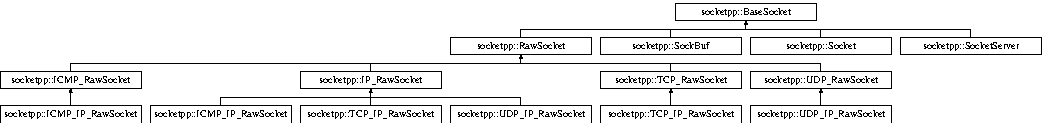
\includegraphics[height=1.64948cm]{classsocketpp_1_1BaseSocket}
\end{center}
\end{figure}
\subsection*{Public Member Functions}
\begin{CompactItemize}
\item 
void \hyperlink{classsocketpp_1_1BaseSocket_2060dc1b648f83f8bf5ae3d9ecfcd619}{open} (\hyperlink{namespacesocketpp_635f4c3b3f85aba331587404d59ae52d}{type} t, \hyperlink{namespacesocketpp_2969678def1c6c8cb4102802ca82e2cf}{protocol} prot=ipproto\_\-ip)
\begin{CompactList}\small\item\em opens socket descriptor \item\end{CompactList}\item 
virtual void \hyperlink{classsocketpp_1_1BaseSocket_f067195056bb6b5a65c4bc1d2ac7da72}{close} ()
\begin{CompactList}\small\item\em closes socket descriptor \item\end{CompactList}\item 
void \hyperlink{classsocketpp_1_1BaseSocket_4cffcd5cae4ef51e953495837fade4c3}{setBlocking} (bool yes)
\item 
{\footnotesize template$<$typename T $>$ }\\int \hyperlink{classsocketpp_1_1BaseSocket_c845c3a037f0f400fd50dfb58706b6e4}{getsockopt} (\hyperlink{namespacesocketpp_4dbb83d08769b55fc6e283b73ae11bb5}{level} lev, \hyperlink{namespacesocketpp_ea335944de1f6b81489c90507884cfc4}{option} opt, T \&optval)
\begin{CompactList}\small\item\em gets options set on socket descriptor. Wrapper for \hyperlink{classsocketpp_1_1BaseSocket_c845c3a037f0f400fd50dfb58706b6e4}{getsockopt()} \item\end{CompactList}\item 
{\footnotesize template$<$typename T $>$ }\\int \hyperlink{classsocketpp_1_1BaseSocket_3f1f168e4953c046bb1159941da2fa30}{setsockopt} (\hyperlink{namespacesocketpp_4dbb83d08769b55fc6e283b73ae11bb5}{level} lev, \hyperlink{namespacesocketpp_ea335944de1f6b81489c90507884cfc4}{option} opt, const T \&optval)
\begin{CompactList}\small\item\em sets options set on socket descriptor. Wrapper for \hyperlink{classsocketpp_1_1BaseSocket_3f1f168e4953c046bb1159941da2fa30}{setsockopt()} \item\end{CompactList}\item 
int \hyperlink{classsocketpp_1_1BaseSocket_769710192256606aaec1a776468d75fa}{connect} (const std::string \&addr, \hyperlink{namespacesocketpp_5517ef80f249b891a2ba64b95fc1e723}{port\_\-t} port=0)
\begin{CompactList}\small\item\em connects socket to remote address \item\end{CompactList}\item 
int \hyperlink{classsocketpp_1_1BaseSocket_2bdd6d459e6f9cf2f71636b01787b250}{connect} (in\_\-addr\_\-t addr, \hyperlink{namespacesocketpp_5517ef80f249b891a2ba64b95fc1e723}{port\_\-t} port=0)
\begin{CompactList}\small\item\em connects socket to remote address \item\end{CompactList}\item 
int \hyperlink{classsocketpp_1_1BaseSocket_eb0f4c84546c22fd9023169701d8fae8}{connect} (const std::string \&addr, const std::string \&serv, const char $\ast$prot=NULL)
\begin{CompactList}\small\item\em connects socket to remote address \item\end{CompactList}\item 
int \hyperlink{classsocketpp_1_1BaseSocket_83666b030a93368675a842a992e0c2af}{connect} (in\_\-addr\_\-t addr, const std::string \&serv, const char $\ast$prot=NULL)
\begin{CompactList}\small\item\em connects socket to remote address \item\end{CompactList}\item 
int \hyperlink{classsocketpp_1_1BaseSocket_78c2a8e6a5c7dfbc708c9cd637e88e51}{bind} (const std::string \&addr, \hyperlink{namespacesocketpp_5517ef80f249b891a2ba64b95fc1e723}{port\_\-t} port=0)
\begin{CompactList}\small\item\em binds socket to local given address \item\end{CompactList}\item 
int \hyperlink{classsocketpp_1_1BaseSocket_d3df73f534900d40f9dff26171ec93b5}{bind} (in\_\-addr\_\-t addr, \hyperlink{namespacesocketpp_5517ef80f249b891a2ba64b95fc1e723}{port\_\-t} port=0)
\begin{CompactList}\small\item\em binds socket to local given address \item\end{CompactList}\item 
int \hyperlink{classsocketpp_1_1BaseSocket_4775f13f8e1cceaaed40106162b2149f}{bind} (const std::string \&addr, const std::string \&serv, const char $\ast$prot=NULL)
\begin{CompactList}\small\item\em binds socket to local given address \item\end{CompactList}\item 
int \hyperlink{classsocketpp_1_1BaseSocket_aab800bcb5ee48cd4410ae2b9ed83e23}{bind} (in\_\-addr\_\-t addr, const std::string \&serv, const char $\ast$prot=NULL)
\begin{CompactList}\small\item\em binds socket to local given address \item\end{CompactList}\item 
void \hyperlink{classsocketpp_1_1BaseSocket_0804d148470fd742cda495d3533b25c6}{settimeout} (double time)
\begin{CompactList}\small\item\em sets \hyperlink{classsocketpp_1_1timeout}{timeout} on the following IO operations. If time is 0 \hyperlink{classsocketpp_1_1timeout}{timeout} is cancelled. \item\end{CompactList}\item 
std::string \hyperlink{classsocketpp_1_1BaseSocket_483c6186ae60d0c399983e14f55af600}{remoteAddr} ()
\begin{CompactList}\small\item\em returns remote address to which socket is connected \item\end{CompactList}\item 
std::string \hyperlink{classsocketpp_1_1BaseSocket_0caed2e7d3f0e4db7d4c1aa3aba52caf}{localAddr} ()
\begin{CompactList}\small\item\em returns local address to which socket is bound \item\end{CompactList}\item 
\hyperlink{namespacesocketpp_5517ef80f249b891a2ba64b95fc1e723}{port\_\-t} \hyperlink{classsocketpp_1_1BaseSocket_d4a2c0e4932436ef61f911514385d16c}{localPort} ()
\begin{CompactList}\small\item\em returns local port to which socket is bound \item\end{CompactList}\item 
\hyperlink{namespacesocketpp_5517ef80f249b891a2ba64b95fc1e723}{port\_\-t} \hyperlink{classsocketpp_1_1BaseSocket_039db642444d2111f2f58ebe032c5f5f}{remotePort} ()
\begin{CompactList}\small\item\em returns remote port bound to which socket is connected \item\end{CompactList}\item 
int \hyperlink{classsocketpp_1_1BaseSocket_c96db07cc917926d895d89cf73734ea1}{fileno} () const 
\begin{CompactList}\small\item\em returns socket descriptor number \item\end{CompactList}\item 
\hyperlink{classsocketpp_1_1BaseSocket_fa397f810462fe61238dbbf2d9c42c90}{operator int} () const 
\begin{CompactList}\small\item\em calls \hyperlink{classsocketpp_1_1BaseSocket_c96db07cc917926d895d89cf73734ea1}{fileno()} \item\end{CompactList}\item 
void \hyperlink{classsocketpp_1_1BaseSocket_f3a4c01a7bf911460296a873ce0913da}{cleanDnsCache} ()
\begin{CompactList}\small\item\em cleans internal DNS cache \item\end{CompactList}\item 
std::map$<$ std::string, std::string $>$ \hyperlink{classsocketpp_1_1BaseSocket_52bf8df48bf4da48eff4adc690caa211}{getDnsCache} ()
\begin{CompactList}\small\item\em returns internal DNS cache \item\end{CompactList}\item 
virtual \hyperlink{classsocketpp_1_1BaseSocket_2e066addfaa6f5648e68b3e6b0a15e79}{$\sim$BaseSocket} ()
\begin{CompactList}\small\item\em desctuctor which calls \hyperlink{classsocketpp_1_1BaseSocket_f067195056bb6b5a65c4bc1d2ac7da72}{close()} \item\end{CompactList}\end{CompactItemize}
\subsection*{Protected Types}
\begin{CompactItemize}
\item 
enum \hyperlink{classsocketpp_1_1BaseSocket_21492d478c5aa2ff8a1ad258ccf58062}{\_\-select\_\-mode} \{ \hyperlink{classsocketpp_1_1BaseSocket_21492d478c5aa2ff8a1ad258ccf580624782d25091b1ee2cda4f94b131593ce6}{read}, 
\hyperlink{classsocketpp_1_1BaseSocket_21492d478c5aa2ff8a1ad258ccf58062a19a7e61ac1d2a5dcb0efb4f71795685}{write}, 
\hyperlink{classsocketpp_1_1BaseSocket_21492d478c5aa2ff8a1ad258ccf58062401c7b14b3583749a9a5234ff43cb1c4}{err}
 \}
\subsection*{Protected Member Functions}
\begin{CompactItemize}
\item 
\hyperlink{classsocketpp_1_1BaseSocket_3eb81ecbf94ce83afa6b2f60206c77f2}{BaseSocket} ()
\begin{CompactList}\small\item\em simply instantiates the class without setting the internal socket descriptor \item\end{CompactList}\item 
\hyperlink{classsocketpp_1_1BaseSocket_0c142db99422572579c91f3e176035c6}{BaseSocket} (const \hyperlink{classsocketpp_1_1BaseSocket}{BaseSocket} \&s)
\begin{CompactList}\small\item\em copy constructor \item\end{CompactList}\item 
\hyperlink{classsocketpp_1_1BaseSocket_35c982d7aef2041c100439cf38aa7f4d}{BaseSocket} (\hyperlink{namespacesocketpp_635f4c3b3f85aba331587404d59ae52d}{type} t, \hyperlink{namespacesocketpp_2969678def1c6c8cb4102802ca82e2cf}{protocol} prot=ipproto\_\-ip)
\begin{CompactList}\small\item\em constructor which opens the socket descriptor calling socket(AF\_\-INET, t, prot) \item\end{CompactList}\item 
\hyperlink{classsocketpp_1_1BaseSocket_f7e18d6700868abb2b476e797506eafb}{BaseSocket} (int fd)
\begin{CompactList}\small\item\em constructor which uses the given socket descriptor \item\end{CompactList}\item 
int \hyperlink{classsocketpp_1_1BaseSocket_9c925091102c9371be9990fedd605f1c}{\_\-select} (\hyperlink{classsocketpp_1_1BaseSocket_21492d478c5aa2ff8a1ad258ccf58062}{\_\-select\_\-mode} m)
\item 
size\_\-t \hyperlink{classsocketpp_1_1BaseSocket_bf4e15b88271e34e606b9b2a5b384b5b}{send} (const char buf\mbox{[}$\,$\mbox{]}, size\_\-t size)
\begin{CompactList}\small\item\em sends data over socket \item\end{CompactList}\item 
size\_\-t \hyperlink{classsocketpp_1_1BaseSocket_08b3e29d019575293fa134c6d91d6cbb}{recv} (char buf\mbox{[}$\,$\mbox{]}, size\_\-t size)
\begin{CompactList}\small\item\em reads data on socket \item\end{CompactList}\item 
size\_\-t \hyperlink{classsocketpp_1_1BaseSocket_fb896f016a243ddbb661acc7b05826bf}{send} (const std::string \&buf)
\begin{CompactList}\small\item\em sends data over socket \item\end{CompactList}\item 
size\_\-t \hyperlink{classsocketpp_1_1BaseSocket_25fc62d259f6d12f1b1a5001a7512897}{recv} (std::string \&buf, size\_\-t size)
\begin{CompactList}\small\item\em reads data on socket \item\end{CompactList}\item 
size\_\-t \hyperlink{classsocketpp_1_1BaseSocket_33ef257bb6eb0f23ae0680df57738f3a}{sendto} (const char buf\mbox{[}$\,$\mbox{]}, size\_\-t size, in\_\-addr\_\-t addr, \hyperlink{namespacesocketpp_5517ef80f249b891a2ba64b95fc1e723}{port\_\-t} port=0)
\begin{CompactList}\small\item\em sends data over socket \item\end{CompactList}\item 
size\_\-t \hyperlink{classsocketpp_1_1BaseSocket_d12e08b6f67a95a3181403c70f306f88}{sendto} (const std::string \&buf, in\_\-addr\_\-t addr, \hyperlink{namespacesocketpp_5517ef80f249b891a2ba64b95fc1e723}{port\_\-t} port=0)
\begin{CompactList}\small\item\em sends data over socket \item\end{CompactList}\item 
size\_\-t \hyperlink{classsocketpp_1_1BaseSocket_2b591cefe9fd8ac9f46ed7fbdd8caa82}{sendto} (const char buf\mbox{[}$\,$\mbox{]}, size\_\-t size, const std::string \&addr, \hyperlink{namespacesocketpp_5517ef80f249b891a2ba64b95fc1e723}{port\_\-t} port=0)
\begin{CompactList}\small\item\em sends data over socket \item\end{CompactList}\item 
size\_\-t \hyperlink{classsocketpp_1_1BaseSocket_8f98eff253e52ccf3463a0379a10caf2}{sendto} (const std::string \&buf, const std::string \&addr, \hyperlink{namespacesocketpp_5517ef80f249b891a2ba64b95fc1e723}{port\_\-t} port=0)
\begin{CompactList}\small\item\em sends data over socket \item\end{CompactList}\item 
size\_\-t \hyperlink{classsocketpp_1_1BaseSocket_0154d562be27c8b2aa074d5f6bb8ab03}{sendto} (const char buf\mbox{[}$\,$\mbox{]}, size\_\-t size, in\_\-addr\_\-t addr, const std::string \&serv, const char $\ast$prot=NULL)
\begin{CompactList}\small\item\em sends data over socket \item\end{CompactList}\item 
size\_\-t \hyperlink{classsocketpp_1_1BaseSocket_4afc9ac34b702af852f2b52e68a90c3e}{sendto} (const std::string \&buf, in\_\-addr\_\-t addr, const std::string \&serv, const char $\ast$prot=NULL)
\begin{CompactList}\small\item\em sends data over socket \item\end{CompactList}\item 
size\_\-t \hyperlink{classsocketpp_1_1BaseSocket_c0bbca9725a55a2e6a822536efd31b73}{sendto} (const char buf\mbox{[}$\,$\mbox{]}, size\_\-t size, const std::string \&addr, const std::string \&serv, const char $\ast$prot=NULL)
\begin{CompactList}\small\item\em sends data over socket \item\end{CompactList}\item 
size\_\-t \hyperlink{classsocketpp_1_1BaseSocket_5fd9737270ee71d2292e70ed625d63f9}{sendto} (const std::string \&buf, const std::string \&addr, const std::string \&serv, const char $\ast$prot=NULL)
\begin{CompactList}\small\item\em sends data over socket \item\end{CompactList}\item 
size\_\-t \hyperlink{classsocketpp_1_1BaseSocket_11ebe50d7ae76c21ef55d38cb87cc700}{recvfrom} (char buf\mbox{[}$\,$\mbox{]}, size\_\-t size, in\_\-addr\_\-t \&addr, \hyperlink{namespacesocketpp_5517ef80f249b891a2ba64b95fc1e723}{port\_\-t} \&port)
\begin{CompactList}\small\item\em reads data on socket \item\end{CompactList}\item 
size\_\-t \hyperlink{classsocketpp_1_1BaseSocket_d2656c57d84c4ff032cd3d9ad4608bfa}{recvfrom} (std::string \&buf, size\_\-t size, in\_\-addr\_\-t \&addr, \hyperlink{namespacesocketpp_5517ef80f249b891a2ba64b95fc1e723}{port\_\-t} \&port)
\begin{CompactList}\small\item\em reads data on socket \item\end{CompactList}\item 
size\_\-t \hyperlink{classsocketpp_1_1BaseSocket_205fc515468a3df01258f7ebd6fdf38c}{recvfrom} (char buf\mbox{[}$\,$\mbox{]}, size\_\-t size, std::string \&addr, \hyperlink{namespacesocketpp_5517ef80f249b891a2ba64b95fc1e723}{port\_\-t} \&port)
\begin{CompactList}\small\item\em reads data on socket \item\end{CompactList}\item 
size\_\-t \hyperlink{classsocketpp_1_1BaseSocket_259bb054a2abf0ffadf3c75bce4892b0}{recvfrom} (std::string \&buf, size\_\-t size, std::string \&addr, \hyperlink{namespacesocketpp_5517ef80f249b891a2ba64b95fc1e723}{port\_\-t} \&port)
\begin{CompactList}\small\item\em reads data on socket \item\end{CompactList}\item 
size\_\-t \hyperlink{classsocketpp_1_1BaseSocket_ed28eb7e4a5abee65143bcdf162673f4}{recvfrom} (char buf\mbox{[}$\,$\mbox{]}, size\_\-t size, in\_\-addr\_\-t \&addr)
\begin{CompactList}\small\item\em reads data on socket \item\end{CompactList}\item 
size\_\-t \hyperlink{classsocketpp_1_1BaseSocket_8224b8434da862a72b774a3c80006fcb}{recvfrom} (std::string \&buf, size\_\-t size, in\_\-addr\_\-t \&addr)
\begin{CompactList}\small\item\em reads data on socket \item\end{CompactList}\item 
size\_\-t \hyperlink{classsocketpp_1_1BaseSocket_c7a79cd90b082806dcafb14fbbd130b8}{recvfrom} (char buf\mbox{[}$\,$\mbox{]}, size\_\-t size, std::string \&addr)
\begin{CompactList}\small\item\em reads data on socket \item\end{CompactList}\item 
size\_\-t \hyperlink{classsocketpp_1_1BaseSocket_ace82407e13a6eee26aa1f5f642d0cfc}{recvfrom} (std::string \&buf, size\_\-t size, std::string \&addr)
\begin{CompactList}\small\item\em reads data on socket \item\end{CompactList}\end{CompactItemize}
\subsection*{Protected Attributes}
\begin{CompactItemize}
\item 
int \hyperlink{classsocketpp_1_1BaseSocket_a5ef6b5fabb3988bced6a23d9631985d}{\_\-sd}
\item 
\hyperlink{classsocketpp_1_1AddrHandler}{AddrHandler} \hyperlink{classsocketpp_1_1BaseSocket_1e44e3c6c2ecd89c2aa716cc62528620}{\_\-h}
\item 
double \hyperlink{classsocketpp_1_1BaseSocket_418af5a1fe752cef38e4c6679780224c}{\_\-timeout}
\end{CompactItemize}


\subsection{Detailed Description}
Abstract base class. 

\subsection{Member Enumeration Documentation}
\hypertarget{classsocketpp_1_1BaseSocket_21492d478c5aa2ff8a1ad258ccf58062}{
\index{socketpp::BaseSocket@{socketpp::BaseSocket}!\_\-select\_\-mode@{\_\-select\_\-mode}}
\index{\_\-select\_\-mode@{\_\-select\_\-mode}!socketpp::BaseSocket@{socketpp::BaseSocket}}
\subsubsection[{\_\-select\_\-mode}]{\setlength{\rightskip}{0pt plus 5cm}enum {\bf socketpp::BaseSocket::\_\-select\_\-mode}\hspace{0.3cm}{\tt  \mbox{[}protected\mbox{]}}}}
\label{classsocketpp_1_1BaseSocket_21492d478c5aa2ff8a1ad258ccf58062}


\begin{Desc}
\item[Enumerator: ]\par
\begin{description}
\index{read@{read}!socketpp::BaseSocket@{socketpp::BaseSocket}}\index{socketpp::BaseSocket@{socketpp::BaseSocket}!read@{read}}\item[{\em 
\hypertarget{classsocketpp_1_1BaseSocket_21492d478c5aa2ff8a1ad258ccf580624782d25091b1ee2cda4f94b131593ce6}{
read}
\label{classsocketpp_1_1BaseSocket_21492d478c5aa2ff8a1ad258ccf580624782d25091b1ee2cda4f94b131593ce6}
}]\index{write@{write}!socketpp::BaseSocket@{socketpp::BaseSocket}}\index{socketpp::BaseSocket@{socketpp::BaseSocket}!write@{write}}\item[{\em 
\hypertarget{classsocketpp_1_1BaseSocket_21492d478c5aa2ff8a1ad258ccf58062a19a7e61ac1d2a5dcb0efb4f71795685}{
write}
\label{classsocketpp_1_1BaseSocket_21492d478c5aa2ff8a1ad258ccf58062a19a7e61ac1d2a5dcb0efb4f71795685}
}]\index{err@{err}!socketpp::BaseSocket@{socketpp::BaseSocket}}\index{socketpp::BaseSocket@{socketpp::BaseSocket}!err@{err}}\item[{\em 
\hypertarget{classsocketpp_1_1BaseSocket_21492d478c5aa2ff8a1ad258ccf58062401c7b14b3583749a9a5234ff43cb1c4}{
err}
\label{classsocketpp_1_1BaseSocket_21492d478c5aa2ff8a1ad258ccf58062401c7b14b3583749a9a5234ff43cb1c4}
}]\end{description}
\end{Desc}



\subsection{Constructor \& Destructor Documentation}
\hypertarget{classsocketpp_1_1BaseSocket_2e066addfaa6f5648e68b3e6b0a15e79}{
\index{socketpp::BaseSocket@{socketpp::BaseSocket}!$\sim$BaseSocket@{$\sim$BaseSocket}}
\index{$\sim$BaseSocket@{$\sim$BaseSocket}!socketpp::BaseSocket@{socketpp::BaseSocket}}
\subsubsection[{$\sim$BaseSocket}]{\setlength{\rightskip}{0pt plus 5cm}socketpp::BaseSocket::$\sim$BaseSocket ()\hspace{0.3cm}{\tt  \mbox{[}virtual\mbox{]}}}}
\label{classsocketpp_1_1BaseSocket_2e066addfaa6f5648e68b3e6b0a15e79}


desctuctor which calls \hyperlink{classsocketpp_1_1BaseSocket_f067195056bb6b5a65c4bc1d2ac7da72}{close()} 

\hypertarget{classsocketpp_1_1BaseSocket_3eb81ecbf94ce83afa6b2f60206c77f2}{
\index{socketpp::BaseSocket@{socketpp::BaseSocket}!BaseSocket@{BaseSocket}}
\index{BaseSocket@{BaseSocket}!socketpp::BaseSocket@{socketpp::BaseSocket}}
\subsubsection[{BaseSocket}]{\setlength{\rightskip}{0pt plus 5cm}socketpp::BaseSocket::BaseSocket ()\hspace{0.3cm}{\tt  \mbox{[}protected\mbox{]}}}}
\label{classsocketpp_1_1BaseSocket_3eb81ecbf94ce83afa6b2f60206c77f2}


simply instantiates the class without setting the internal socket descriptor 

\hypertarget{classsocketpp_1_1BaseSocket_0c142db99422572579c91f3e176035c6}{
\index{socketpp::BaseSocket@{socketpp::BaseSocket}!BaseSocket@{BaseSocket}}
\index{BaseSocket@{BaseSocket}!socketpp::BaseSocket@{socketpp::BaseSocket}}
\subsubsection[{BaseSocket}]{\setlength{\rightskip}{0pt plus 5cm}socketpp::BaseSocket::BaseSocket (const {\bf BaseSocket} \& {\em s})\hspace{0.3cm}{\tt  \mbox{[}protected\mbox{]}}}}
\label{classsocketpp_1_1BaseSocket_0c142db99422572579c91f3e176035c6}


copy constructor 

\hypertarget{classsocketpp_1_1BaseSocket_35c982d7aef2041c100439cf38aa7f4d}{
\index{socketpp::BaseSocket@{socketpp::BaseSocket}!BaseSocket@{BaseSocket}}
\index{BaseSocket@{BaseSocket}!socketpp::BaseSocket@{socketpp::BaseSocket}}
\subsubsection[{BaseSocket}]{\setlength{\rightskip}{0pt plus 5cm}socketpp::BaseSocket::BaseSocket ({\bf type} {\em t}, \/  {\bf protocol} {\em prot} = {\tt ipproto\_\-ip})\hspace{0.3cm}{\tt  \mbox{[}protected\mbox{]}}}}
\label{classsocketpp_1_1BaseSocket_35c982d7aef2041c100439cf38aa7f4d}


constructor which opens the socket descriptor calling socket(AF\_\-INET, t, prot) 

\begin{Desc}
\item[Parameters:]
\begin{description}
\item[{\em t}]socket type \item[{\em prot}]socket protocol \end{description}
\end{Desc}
\hypertarget{classsocketpp_1_1BaseSocket_f7e18d6700868abb2b476e797506eafb}{
\index{socketpp::BaseSocket@{socketpp::BaseSocket}!BaseSocket@{BaseSocket}}
\index{BaseSocket@{BaseSocket}!socketpp::BaseSocket@{socketpp::BaseSocket}}
\subsubsection[{BaseSocket}]{\setlength{\rightskip}{0pt plus 5cm}socketpp::BaseSocket::BaseSocket (int {\em fd})\hspace{0.3cm}{\tt  \mbox{[}protected\mbox{]}}}}
\label{classsocketpp_1_1BaseSocket_f7e18d6700868abb2b476e797506eafb}


constructor which uses the given socket descriptor 

\begin{Desc}
\item[Parameters:]
\begin{description}
\item[{\em fd}]file descriptor \end{description}
\end{Desc}


\subsection{Member Function Documentation}
\hypertarget{classsocketpp_1_1BaseSocket_9c925091102c9371be9990fedd605f1c}{
\index{socketpp::BaseSocket@{socketpp::BaseSocket}!\_\-select@{\_\-select}}
\index{\_\-select@{\_\-select}!socketpp::BaseSocket@{socketpp::BaseSocket}}
\subsubsection[{\_\-select}]{\setlength{\rightskip}{0pt plus 5cm}int socketpp::BaseSocket::\_\-select ({\bf \_\-select\_\-mode} {\em m})\hspace{0.3cm}{\tt  \mbox{[}protected\mbox{]}}}}
\label{classsocketpp_1_1BaseSocket_9c925091102c9371be9990fedd605f1c}


\hypertarget{classsocketpp_1_1BaseSocket_aab800bcb5ee48cd4410ae2b9ed83e23}{
\index{socketpp::BaseSocket@{socketpp::BaseSocket}!bind@{bind}}
\index{bind@{bind}!socketpp::BaseSocket@{socketpp::BaseSocket}}
\subsubsection[{bind}]{\setlength{\rightskip}{0pt plus 5cm}int socketpp::BaseSocket::bind (in\_\-addr\_\-t {\em addr}, \/  const std::string \& {\em serv}, \/  const char $\ast$ {\em prot} = {\tt NULL})}}
\label{classsocketpp_1_1BaseSocket_aab800bcb5ee48cd4410ae2b9ed83e23}


binds socket to local given address 

\begin{Desc}
\item[Parameters:]
\begin{description}
\item[{\em addr}]IPv4 numerical address \item[{\em serv}]service name \item[{\em prot}]transport layer protocol \end{description}
\end{Desc}
\begin{Desc}
\item[Returns:]\hyperlink{classsocketpp_1_1BaseSocket_78c2a8e6a5c7dfbc708c9cd637e88e51}{bind()} return value \end{Desc}
\hypertarget{classsocketpp_1_1BaseSocket_4775f13f8e1cceaaed40106162b2149f}{
\index{socketpp::BaseSocket@{socketpp::BaseSocket}!bind@{bind}}
\index{bind@{bind}!socketpp::BaseSocket@{socketpp::BaseSocket}}
\subsubsection[{bind}]{\setlength{\rightskip}{0pt plus 5cm}int socketpp::BaseSocket::bind (const std::string \& {\em addr}, \/  const std::string \& {\em serv}, \/  const char $\ast$ {\em prot} = {\tt NULL})}}
\label{classsocketpp_1_1BaseSocket_4775f13f8e1cceaaed40106162b2149f}


binds socket to local given address 

\begin{Desc}
\item[Parameters:]
\begin{description}
\item[{\em addr}]IPv4 dotted decimal address \item[{\em serv}]service name \item[{\em prot}]transport layer protocol \end{description}
\end{Desc}
\begin{Desc}
\item[Returns:]\hyperlink{classsocketpp_1_1BaseSocket_78c2a8e6a5c7dfbc708c9cd637e88e51}{bind()} return value \end{Desc}
\hypertarget{classsocketpp_1_1BaseSocket_d3df73f534900d40f9dff26171ec93b5}{
\index{socketpp::BaseSocket@{socketpp::BaseSocket}!bind@{bind}}
\index{bind@{bind}!socketpp::BaseSocket@{socketpp::BaseSocket}}
\subsubsection[{bind}]{\setlength{\rightskip}{0pt plus 5cm}int socketpp::BaseSocket::bind (in\_\-addr\_\-t {\em addr}, \/  {\bf port\_\-t} {\em port} = {\tt 0})}}
\label{classsocketpp_1_1BaseSocket_d3df73f534900d40f9dff26171ec93b5}


binds socket to local given address 

\begin{Desc}
\item[Parameters:]
\begin{description}
\item[{\em addr}]IPv4 numerical address \item[{\em port}]port number \end{description}
\end{Desc}
\begin{Desc}
\item[Returns:]\hyperlink{classsocketpp_1_1BaseSocket_78c2a8e6a5c7dfbc708c9cd637e88e51}{bind()} return value \end{Desc}
\hypertarget{classsocketpp_1_1BaseSocket_78c2a8e6a5c7dfbc708c9cd637e88e51}{
\index{socketpp::BaseSocket@{socketpp::BaseSocket}!bind@{bind}}
\index{bind@{bind}!socketpp::BaseSocket@{socketpp::BaseSocket}}
\subsubsection[{bind}]{\setlength{\rightskip}{0pt plus 5cm}int socketpp::BaseSocket::bind (const std::string \& {\em addr}, \/  {\bf port\_\-t} {\em port} = {\tt 0})}}
\label{classsocketpp_1_1BaseSocket_78c2a8e6a5c7dfbc708c9cd637e88e51}


binds socket to local given address 

\begin{Desc}
\item[Parameters:]
\begin{description}
\item[{\em addr}]IPv4 dotted decimal address \item[{\em port}]port number \end{description}
\end{Desc}
\begin{Desc}
\item[Returns:]\hyperlink{classsocketpp_1_1BaseSocket_78c2a8e6a5c7dfbc708c9cd637e88e51}{bind()} return value \end{Desc}
\hypertarget{classsocketpp_1_1BaseSocket_f3a4c01a7bf911460296a873ce0913da}{
\index{socketpp::BaseSocket@{socketpp::BaseSocket}!cleanDnsCache@{cleanDnsCache}}
\index{cleanDnsCache@{cleanDnsCache}!socketpp::BaseSocket@{socketpp::BaseSocket}}
\subsubsection[{cleanDnsCache}]{\setlength{\rightskip}{0pt plus 5cm}void socketpp::BaseSocket::cleanDnsCache ()\hspace{0.3cm}{\tt  \mbox{[}inline\mbox{]}}}}
\label{classsocketpp_1_1BaseSocket_f3a4c01a7bf911460296a873ce0913da}


cleans internal DNS cache 

\hypertarget{classsocketpp_1_1BaseSocket_f067195056bb6b5a65c4bc1d2ac7da72}{
\index{socketpp::BaseSocket@{socketpp::BaseSocket}!close@{close}}
\index{close@{close}!socketpp::BaseSocket@{socketpp::BaseSocket}}
\subsubsection[{close}]{\setlength{\rightskip}{0pt plus 5cm}void socketpp::BaseSocket::close ()\hspace{0.3cm}{\tt  \mbox{[}virtual\mbox{]}}}}
\label{classsocketpp_1_1BaseSocket_f067195056bb6b5a65c4bc1d2ac7da72}


closes socket descriptor 



Reimplemented in \hyperlink{classsocketpp_1_1SockBuf_28f88c6ac0570ee5e9d57e255733b0f9}{socketpp::SockBuf}.\hypertarget{classsocketpp_1_1BaseSocket_83666b030a93368675a842a992e0c2af}{
\index{socketpp::BaseSocket@{socketpp::BaseSocket}!connect@{connect}}
\index{connect@{connect}!socketpp::BaseSocket@{socketpp::BaseSocket}}
\subsubsection[{connect}]{\setlength{\rightskip}{0pt plus 5cm}int socketpp::BaseSocket::connect (in\_\-addr\_\-t {\em addr}, \/  const std::string \& {\em serv}, \/  const char $\ast$ {\em prot} = {\tt NULL})}}
\label{classsocketpp_1_1BaseSocket_83666b030a93368675a842a992e0c2af}


connects socket to remote address 

\begin{Desc}
\item[Parameters:]
\begin{description}
\item[{\em addr}]IPv4 numerical address \item[{\em serv}]service name \item[{\em prot}]transport layer protocol \end{description}
\end{Desc}
\begin{Desc}
\item[Returns:]\hyperlink{classsocketpp_1_1BaseSocket_769710192256606aaec1a776468d75fa}{connect()} return value \end{Desc}
\hypertarget{classsocketpp_1_1BaseSocket_eb0f4c84546c22fd9023169701d8fae8}{
\index{socketpp::BaseSocket@{socketpp::BaseSocket}!connect@{connect}}
\index{connect@{connect}!socketpp::BaseSocket@{socketpp::BaseSocket}}
\subsubsection[{connect}]{\setlength{\rightskip}{0pt plus 5cm}int socketpp::BaseSocket::connect (const std::string \& {\em addr}, \/  const std::string \& {\em serv}, \/  const char $\ast$ {\em prot} = {\tt NULL})}}
\label{classsocketpp_1_1BaseSocket_eb0f4c84546c22fd9023169701d8fae8}


connects socket to remote address 

\begin{Desc}
\item[Parameters:]
\begin{description}
\item[{\em addr}]IPv4 dotted decimal address \item[{\em serv}]service name \item[{\em prot}]transport layer protocol \end{description}
\end{Desc}
\begin{Desc}
\item[Returns:]\hyperlink{classsocketpp_1_1BaseSocket_769710192256606aaec1a776468d75fa}{connect()} return value \end{Desc}
\hypertarget{classsocketpp_1_1BaseSocket_2bdd6d459e6f9cf2f71636b01787b250}{
\index{socketpp::BaseSocket@{socketpp::BaseSocket}!connect@{connect}}
\index{connect@{connect}!socketpp::BaseSocket@{socketpp::BaseSocket}}
\subsubsection[{connect}]{\setlength{\rightskip}{0pt plus 5cm}int socketpp::BaseSocket::connect (in\_\-addr\_\-t {\em addr}, \/  {\bf port\_\-t} {\em port} = {\tt 0})}}
\label{classsocketpp_1_1BaseSocket_2bdd6d459e6f9cf2f71636b01787b250}


connects socket to remote address 

\begin{Desc}
\item[Parameters:]
\begin{description}
\item[{\em addr}]IPv4 numerical address \item[{\em port}]port number \end{description}
\end{Desc}
\begin{Desc}
\item[Returns:]\hyperlink{classsocketpp_1_1BaseSocket_769710192256606aaec1a776468d75fa}{connect()} return value \end{Desc}
\hypertarget{classsocketpp_1_1BaseSocket_769710192256606aaec1a776468d75fa}{
\index{socketpp::BaseSocket@{socketpp::BaseSocket}!connect@{connect}}
\index{connect@{connect}!socketpp::BaseSocket@{socketpp::BaseSocket}}
\subsubsection[{connect}]{\setlength{\rightskip}{0pt plus 5cm}int socketpp::BaseSocket::connect (const std::string \& {\em addr}, \/  {\bf port\_\-t} {\em port} = {\tt 0})}}
\label{classsocketpp_1_1BaseSocket_769710192256606aaec1a776468d75fa}


connects socket to remote address 

\begin{Desc}
\item[Parameters:]
\begin{description}
\item[{\em addr}]IPv4 dotted decimal address \item[{\em port}]port number \end{description}
\end{Desc}
\begin{Desc}
\item[Returns:]\hyperlink{classsocketpp_1_1BaseSocket_769710192256606aaec1a776468d75fa}{connect()} return value \end{Desc}
\hypertarget{classsocketpp_1_1BaseSocket_c96db07cc917926d895d89cf73734ea1}{
\index{socketpp::BaseSocket@{socketpp::BaseSocket}!fileno@{fileno}}
\index{fileno@{fileno}!socketpp::BaseSocket@{socketpp::BaseSocket}}
\subsubsection[{fileno}]{\setlength{\rightskip}{0pt plus 5cm}int socketpp::BaseSocket::fileno () const\hspace{0.3cm}{\tt  \mbox{[}inline\mbox{]}}}}
\label{classsocketpp_1_1BaseSocket_c96db07cc917926d895d89cf73734ea1}


returns socket descriptor number 

\begin{Desc}
\item[Returns:]descriptor number \end{Desc}
\hypertarget{classsocketpp_1_1BaseSocket_52bf8df48bf4da48eff4adc690caa211}{
\index{socketpp::BaseSocket@{socketpp::BaseSocket}!getDnsCache@{getDnsCache}}
\index{getDnsCache@{getDnsCache}!socketpp::BaseSocket@{socketpp::BaseSocket}}
\subsubsection[{getDnsCache}]{\setlength{\rightskip}{0pt plus 5cm}std::map$<$std::string,std::string$>$ socketpp::BaseSocket::getDnsCache ()\hspace{0.3cm}{\tt  \mbox{[}inline\mbox{]}}}}
\label{classsocketpp_1_1BaseSocket_52bf8df48bf4da48eff4adc690caa211}


returns internal DNS cache 

\begin{Desc}
\item[Returns:]DNS cache \end{Desc}
\hypertarget{classsocketpp_1_1BaseSocket_c845c3a037f0f400fd50dfb58706b6e4}{
\index{socketpp::BaseSocket@{socketpp::BaseSocket}!getsockopt@{getsockopt}}
\index{getsockopt@{getsockopt}!socketpp::BaseSocket@{socketpp::BaseSocket}}
\subsubsection[{getsockopt}]{\setlength{\rightskip}{0pt plus 5cm}template$<$typename T $>$ int socketpp::BaseSocket::getsockopt ({\bf level} {\em lev}, \/  {\bf option} {\em opt}, \/  T \& {\em optval})\hspace{0.3cm}{\tt  \mbox{[}inline\mbox{]}}}}
\label{classsocketpp_1_1BaseSocket_c845c3a037f0f400fd50dfb58706b6e4}


gets options set on socket descriptor. Wrapper for \hyperlink{classsocketpp_1_1BaseSocket_c845c3a037f0f400fd50dfb58706b6e4}{getsockopt()} 

\begin{Desc}
\item[Parameters:]
\begin{description}
\item[{\em lev}]\hyperlink{classsocketpp_1_1BaseSocket_c845c3a037f0f400fd50dfb58706b6e4}{getsockopt()} level \item[{\em opt}]\hyperlink{classsocketpp_1_1BaseSocket_c845c3a037f0f400fd50dfb58706b6e4}{getsockopt()} option type \item[{\em optval}]field filled by option value \end{description}
\end{Desc}
\begin{Desc}
\item[Returns:]\hyperlink{classsocketpp_1_1BaseSocket_c845c3a037f0f400fd50dfb58706b6e4}{getsockopt()} return value \end{Desc}
\hypertarget{classsocketpp_1_1BaseSocket_0caed2e7d3f0e4db7d4c1aa3aba52caf}{
\index{socketpp::BaseSocket@{socketpp::BaseSocket}!localAddr@{localAddr}}
\index{localAddr@{localAddr}!socketpp::BaseSocket@{socketpp::BaseSocket}}
\subsubsection[{localAddr}]{\setlength{\rightskip}{0pt plus 5cm}std::string socketpp::BaseSocket::localAddr ()}}
\label{classsocketpp_1_1BaseSocket_0caed2e7d3f0e4db7d4c1aa3aba52caf}


returns local address to which socket is bound 

\begin{Desc}
\item[Returns:]IPv4 dotted decimal address \end{Desc}
\hypertarget{classsocketpp_1_1BaseSocket_d4a2c0e4932436ef61f911514385d16c}{
\index{socketpp::BaseSocket@{socketpp::BaseSocket}!localPort@{localPort}}
\index{localPort@{localPort}!socketpp::BaseSocket@{socketpp::BaseSocket}}
\subsubsection[{localPort}]{\setlength{\rightskip}{0pt plus 5cm}{\bf port\_\-t} socketpp::BaseSocket::localPort ()}}
\label{classsocketpp_1_1BaseSocket_d4a2c0e4932436ef61f911514385d16c}


returns local port to which socket is bound 

\begin{Desc}
\item[Returns:]port number \end{Desc}
\hypertarget{classsocketpp_1_1BaseSocket_2060dc1b648f83f8bf5ae3d9ecfcd619}{
\index{socketpp::BaseSocket@{socketpp::BaseSocket}!open@{open}}
\index{open@{open}!socketpp::BaseSocket@{socketpp::BaseSocket}}
\subsubsection[{open}]{\setlength{\rightskip}{0pt plus 5cm}void socketpp::BaseSocket::open ({\bf type} {\em t}, \/  {\bf protocol} {\em prot} = {\tt ipproto\_\-ip})}}
\label{classsocketpp_1_1BaseSocket_2060dc1b648f83f8bf5ae3d9ecfcd619}


opens socket descriptor 

\begin{Desc}
\item[Parameters:]
\begin{description}
\item[{\em t}]socket type \item[{\em prot}]socket protocol \end{description}
\end{Desc}
\hypertarget{classsocketpp_1_1BaseSocket_fa397f810462fe61238dbbf2d9c42c90}{
\index{socketpp::BaseSocket@{socketpp::BaseSocket}!operator int@{operator int}}
\index{operator int@{operator int}!socketpp::BaseSocket@{socketpp::BaseSocket}}
\subsubsection[{operator int}]{\setlength{\rightskip}{0pt plus 5cm}socketpp::BaseSocket::operator int () const\hspace{0.3cm}{\tt  \mbox{[}inline\mbox{]}}}}
\label{classsocketpp_1_1BaseSocket_fa397f810462fe61238dbbf2d9c42c90}


calls \hyperlink{classsocketpp_1_1BaseSocket_c96db07cc917926d895d89cf73734ea1}{fileno()} 

\hypertarget{classsocketpp_1_1BaseSocket_25fc62d259f6d12f1b1a5001a7512897}{
\index{socketpp::BaseSocket@{socketpp::BaseSocket}!recv@{recv}}
\index{recv@{recv}!socketpp::BaseSocket@{socketpp::BaseSocket}}
\subsubsection[{recv}]{\setlength{\rightskip}{0pt plus 5cm}size\_\-t socketpp::BaseSocket::recv (std::string \& {\em buf}, \/  size\_\-t {\em size})\hspace{0.3cm}{\tt  \mbox{[}protected\mbox{]}}}}
\label{classsocketpp_1_1BaseSocket_25fc62d259f6d12f1b1a5001a7512897}


reads data on socket 

\begin{Desc}
\item[Parameters:]
\begin{description}
\item[{\em buf}]string to fill with data \item[{\em size}]max number of bytes to read \end{description}
\end{Desc}
\begin{Desc}
\item[Returns:]number of bytes received \end{Desc}
\hypertarget{classsocketpp_1_1BaseSocket_08b3e29d019575293fa134c6d91d6cbb}{
\index{socketpp::BaseSocket@{socketpp::BaseSocket}!recv@{recv}}
\index{recv@{recv}!socketpp::BaseSocket@{socketpp::BaseSocket}}
\subsubsection[{recv}]{\setlength{\rightskip}{0pt plus 5cm}size\_\-t socketpp::BaseSocket::recv (char {\em buf}\mbox{[}$\,$\mbox{]}, \/  size\_\-t {\em size})\hspace{0.3cm}{\tt  \mbox{[}protected\mbox{]}}}}
\label{classsocketpp_1_1BaseSocket_08b3e29d019575293fa134c6d91d6cbb}


reads data on socket 

\begin{Desc}
\item[Parameters:]
\begin{description}
\item[{\em buf}]buffer to fill with data \item[{\em size}]max number of bytes to read \end{description}
\end{Desc}
\begin{Desc}
\item[Returns:]number of bytes received \end{Desc}
\hypertarget{classsocketpp_1_1BaseSocket_ace82407e13a6eee26aa1f5f642d0cfc}{
\index{socketpp::BaseSocket@{socketpp::BaseSocket}!recvfrom@{recvfrom}}
\index{recvfrom@{recvfrom}!socketpp::BaseSocket@{socketpp::BaseSocket}}
\subsubsection[{recvfrom}]{\setlength{\rightskip}{0pt plus 5cm}size\_\-t socketpp::BaseSocket::recvfrom (std::string \& {\em buf}, \/  size\_\-t {\em size}, \/  std::string \& {\em addr})\hspace{0.3cm}{\tt  \mbox{[}protected\mbox{]}}}}
\label{classsocketpp_1_1BaseSocket_ace82407e13a6eee26aa1f5f642d0cfc}


reads data on socket 

\begin{Desc}
\item[Parameters:]
\begin{description}
\item[{\em buf}]string to fill with data \item[{\em size}]max number of bytes to read \item[{\em addr}]field filled with dotted decimal remote address \end{description}
\end{Desc}
\begin{Desc}
\item[Returns:]number of bytes received \end{Desc}
\hypertarget{classsocketpp_1_1BaseSocket_c7a79cd90b082806dcafb14fbbd130b8}{
\index{socketpp::BaseSocket@{socketpp::BaseSocket}!recvfrom@{recvfrom}}
\index{recvfrom@{recvfrom}!socketpp::BaseSocket@{socketpp::BaseSocket}}
\subsubsection[{recvfrom}]{\setlength{\rightskip}{0pt plus 5cm}size\_\-t socketpp::BaseSocket::recvfrom (char {\em buf}\mbox{[}$\,$\mbox{]}, \/  size\_\-t {\em size}, \/  std::string \& {\em addr})\hspace{0.3cm}{\tt  \mbox{[}protected\mbox{]}}}}
\label{classsocketpp_1_1BaseSocket_c7a79cd90b082806dcafb14fbbd130b8}


reads data on socket 

\begin{Desc}
\item[Parameters:]
\begin{description}
\item[{\em buf}]buffer to fill with data \item[{\em size}]max number of bytes to read \item[{\em addr}]field filled with dotted decimal remote address \end{description}
\end{Desc}
\begin{Desc}
\item[Returns:]number of bytes received \end{Desc}
\hypertarget{classsocketpp_1_1BaseSocket_8224b8434da862a72b774a3c80006fcb}{
\index{socketpp::BaseSocket@{socketpp::BaseSocket}!recvfrom@{recvfrom}}
\index{recvfrom@{recvfrom}!socketpp::BaseSocket@{socketpp::BaseSocket}}
\subsubsection[{recvfrom}]{\setlength{\rightskip}{0pt plus 5cm}size\_\-t socketpp::BaseSocket::recvfrom (std::string \& {\em buf}, \/  size\_\-t {\em size}, \/  in\_\-addr\_\-t \& {\em addr})\hspace{0.3cm}{\tt  \mbox{[}protected\mbox{]}}}}
\label{classsocketpp_1_1BaseSocket_8224b8434da862a72b774a3c80006fcb}


reads data on socket 

\begin{Desc}
\item[Parameters:]
\begin{description}
\item[{\em buf}]string to fill with data \item[{\em size}]max number of bytes to read \item[{\em addr}]field filled with numerical remote address \end{description}
\end{Desc}
\begin{Desc}
\item[Returns:]number of bytes received \end{Desc}
\hypertarget{classsocketpp_1_1BaseSocket_ed28eb7e4a5abee65143bcdf162673f4}{
\index{socketpp::BaseSocket@{socketpp::BaseSocket}!recvfrom@{recvfrom}}
\index{recvfrom@{recvfrom}!socketpp::BaseSocket@{socketpp::BaseSocket}}
\subsubsection[{recvfrom}]{\setlength{\rightskip}{0pt plus 5cm}size\_\-t socketpp::BaseSocket::recvfrom (char {\em buf}\mbox{[}$\,$\mbox{]}, \/  size\_\-t {\em size}, \/  in\_\-addr\_\-t \& {\em addr})\hspace{0.3cm}{\tt  \mbox{[}protected\mbox{]}}}}
\label{classsocketpp_1_1BaseSocket_ed28eb7e4a5abee65143bcdf162673f4}


reads data on socket 

\begin{Desc}
\item[Parameters:]
\begin{description}
\item[{\em buf}]buffer to fill with data \item[{\em size}]max number of bytes to read \item[{\em addr}]field filled with numerical remote address \end{description}
\end{Desc}
\begin{Desc}
\item[Returns:]number of bytes received \end{Desc}
\hypertarget{classsocketpp_1_1BaseSocket_259bb054a2abf0ffadf3c75bce4892b0}{
\index{socketpp::BaseSocket@{socketpp::BaseSocket}!recvfrom@{recvfrom}}
\index{recvfrom@{recvfrom}!socketpp::BaseSocket@{socketpp::BaseSocket}}
\subsubsection[{recvfrom}]{\setlength{\rightskip}{0pt plus 5cm}size\_\-t socketpp::BaseSocket::recvfrom (std::string \& {\em buf}, \/  size\_\-t {\em size}, \/  std::string \& {\em addr}, \/  {\bf port\_\-t} \& {\em port})\hspace{0.3cm}{\tt  \mbox{[}protected\mbox{]}}}}
\label{classsocketpp_1_1BaseSocket_259bb054a2abf0ffadf3c75bce4892b0}


reads data on socket 

\begin{Desc}
\item[Parameters:]
\begin{description}
\item[{\em buf}]string to fill with data \item[{\em size}]max number of bytes to read \item[{\em addr}]field filled with dotted decimal remote address \item[{\em port}]field filled with remote port \end{description}
\end{Desc}
\begin{Desc}
\item[Returns:]number of bytes received \end{Desc}
\hypertarget{classsocketpp_1_1BaseSocket_205fc515468a3df01258f7ebd6fdf38c}{
\index{socketpp::BaseSocket@{socketpp::BaseSocket}!recvfrom@{recvfrom}}
\index{recvfrom@{recvfrom}!socketpp::BaseSocket@{socketpp::BaseSocket}}
\subsubsection[{recvfrom}]{\setlength{\rightskip}{0pt plus 5cm}size\_\-t socketpp::BaseSocket::recvfrom (char {\em buf}\mbox{[}$\,$\mbox{]}, \/  size\_\-t {\em size}, \/  std::string \& {\em addr}, \/  {\bf port\_\-t} \& {\em port})\hspace{0.3cm}{\tt  \mbox{[}protected\mbox{]}}}}
\label{classsocketpp_1_1BaseSocket_205fc515468a3df01258f7ebd6fdf38c}


reads data on socket 

\begin{Desc}
\item[Parameters:]
\begin{description}
\item[{\em buf}]buffer to fill with data \item[{\em size}]max number of bytes to read \item[{\em addr}]field filled with dotted decimal remote address \item[{\em port}]field filled with remote port \end{description}
\end{Desc}
\begin{Desc}
\item[Returns:]number of bytes received \end{Desc}
\hypertarget{classsocketpp_1_1BaseSocket_d2656c57d84c4ff032cd3d9ad4608bfa}{
\index{socketpp::BaseSocket@{socketpp::BaseSocket}!recvfrom@{recvfrom}}
\index{recvfrom@{recvfrom}!socketpp::BaseSocket@{socketpp::BaseSocket}}
\subsubsection[{recvfrom}]{\setlength{\rightskip}{0pt plus 5cm}size\_\-t socketpp::BaseSocket::recvfrom (std::string \& {\em buf}, \/  size\_\-t {\em size}, \/  in\_\-addr\_\-t \& {\em addr}, \/  {\bf port\_\-t} \& {\em port})\hspace{0.3cm}{\tt  \mbox{[}protected\mbox{]}}}}
\label{classsocketpp_1_1BaseSocket_d2656c57d84c4ff032cd3d9ad4608bfa}


reads data on socket 

\begin{Desc}
\item[Parameters:]
\begin{description}
\item[{\em buf}]string to fill with data \item[{\em size}]max number of bytes to read \item[{\em addr}]field filled with numerical remote address \item[{\em port}]field filled with remote port \end{description}
\end{Desc}
\begin{Desc}
\item[Returns:]number of bytes received \end{Desc}
\hypertarget{classsocketpp_1_1BaseSocket_11ebe50d7ae76c21ef55d38cb87cc700}{
\index{socketpp::BaseSocket@{socketpp::BaseSocket}!recvfrom@{recvfrom}}
\index{recvfrom@{recvfrom}!socketpp::BaseSocket@{socketpp::BaseSocket}}
\subsubsection[{recvfrom}]{\setlength{\rightskip}{0pt plus 5cm}size\_\-t socketpp::BaseSocket::recvfrom (char {\em buf}\mbox{[}$\,$\mbox{]}, \/  size\_\-t {\em size}, \/  in\_\-addr\_\-t \& {\em addr}, \/  {\bf port\_\-t} \& {\em port})\hspace{0.3cm}{\tt  \mbox{[}protected\mbox{]}}}}
\label{classsocketpp_1_1BaseSocket_11ebe50d7ae76c21ef55d38cb87cc700}


reads data on socket 

\begin{Desc}
\item[Parameters:]
\begin{description}
\item[{\em buf}]buffer to fill with data \item[{\em size}]max number of bytes to read \item[{\em addr}]field filled with numerical remote address \item[{\em port}]field filled with remote port \end{description}
\end{Desc}
\begin{Desc}
\item[Returns:]number of bytes received \end{Desc}
\hypertarget{classsocketpp_1_1BaseSocket_483c6186ae60d0c399983e14f55af600}{
\index{socketpp::BaseSocket@{socketpp::BaseSocket}!remoteAddr@{remoteAddr}}
\index{remoteAddr@{remoteAddr}!socketpp::BaseSocket@{socketpp::BaseSocket}}
\subsubsection[{remoteAddr}]{\setlength{\rightskip}{0pt plus 5cm}std::string socketpp::BaseSocket::remoteAddr ()}}
\label{classsocketpp_1_1BaseSocket_483c6186ae60d0c399983e14f55af600}


returns remote address to which socket is connected 

\begin{Desc}
\item[Returns:]IPv4 dotted decimal address \end{Desc}
\hypertarget{classsocketpp_1_1BaseSocket_039db642444d2111f2f58ebe032c5f5f}{
\index{socketpp::BaseSocket@{socketpp::BaseSocket}!remotePort@{remotePort}}
\index{remotePort@{remotePort}!socketpp::BaseSocket@{socketpp::BaseSocket}}
\subsubsection[{remotePort}]{\setlength{\rightskip}{0pt plus 5cm}{\bf port\_\-t} socketpp::BaseSocket::remotePort ()}}
\label{classsocketpp_1_1BaseSocket_039db642444d2111f2f58ebe032c5f5f}


returns remote port bound to which socket is connected 

\begin{Desc}
\item[Returns:]port number \end{Desc}
\hypertarget{classsocketpp_1_1BaseSocket_fb896f016a243ddbb661acc7b05826bf}{
\index{socketpp::BaseSocket@{socketpp::BaseSocket}!send@{send}}
\index{send@{send}!socketpp::BaseSocket@{socketpp::BaseSocket}}
\subsubsection[{send}]{\setlength{\rightskip}{0pt plus 5cm}size\_\-t socketpp::BaseSocket::send (const std::string \& {\em buf})\hspace{0.3cm}{\tt  \mbox{[}protected\mbox{]}}}}
\label{classsocketpp_1_1BaseSocket_fb896f016a243ddbb661acc7b05826bf}


sends data over socket 

\begin{Desc}
\item[Parameters:]
\begin{description}
\item[{\em buf}]data string \end{description}
\end{Desc}
\begin{Desc}
\item[Returns:]number of bytes sent \end{Desc}
\hypertarget{classsocketpp_1_1BaseSocket_bf4e15b88271e34e606b9b2a5b384b5b}{
\index{socketpp::BaseSocket@{socketpp::BaseSocket}!send@{send}}
\index{send@{send}!socketpp::BaseSocket@{socketpp::BaseSocket}}
\subsubsection[{send}]{\setlength{\rightskip}{0pt plus 5cm}size\_\-t socketpp::BaseSocket::send (const char {\em buf}\mbox{[}$\,$\mbox{]}, \/  size\_\-t {\em size})\hspace{0.3cm}{\tt  \mbox{[}protected\mbox{]}}}}
\label{classsocketpp_1_1BaseSocket_bf4e15b88271e34e606b9b2a5b384b5b}


sends data over socket 

\begin{Desc}
\item[Parameters:]
\begin{description}
\item[{\em buf}]data buffer \item[{\em size}]size of data in bytes \end{description}
\end{Desc}
\begin{Desc}
\item[Returns:]number of bytes sent \end{Desc}
\hypertarget{classsocketpp_1_1BaseSocket_5fd9737270ee71d2292e70ed625d63f9}{
\index{socketpp::BaseSocket@{socketpp::BaseSocket}!sendto@{sendto}}
\index{sendto@{sendto}!socketpp::BaseSocket@{socketpp::BaseSocket}}
\subsubsection[{sendto}]{\setlength{\rightskip}{0pt plus 5cm}size\_\-t socketpp::BaseSocket::sendto (const std::string \& {\em buf}, \/  const std::string \& {\em addr}, \/  const std::string \& {\em serv}, \/  const char $\ast$ {\em prot} = {\tt NULL})\hspace{0.3cm}{\tt  \mbox{[}protected\mbox{]}}}}
\label{classsocketpp_1_1BaseSocket_5fd9737270ee71d2292e70ed625d63f9}


sends data over socket 

\begin{Desc}
\item[Parameters:]
\begin{description}
\item[{\em buf}]data string \item[{\em addr}]dotted decimal remote address \item[{\em serv}]service name \item[{\em prot}]transport layer protocol \end{description}
\end{Desc}
\begin{Desc}
\item[Returns:]number of bytes sent \end{Desc}
\hypertarget{classsocketpp_1_1BaseSocket_c0bbca9725a55a2e6a822536efd31b73}{
\index{socketpp::BaseSocket@{socketpp::BaseSocket}!sendto@{sendto}}
\index{sendto@{sendto}!socketpp::BaseSocket@{socketpp::BaseSocket}}
\subsubsection[{sendto}]{\setlength{\rightskip}{0pt plus 5cm}size\_\-t socketpp::BaseSocket::sendto (const char {\em buf}\mbox{[}$\,$\mbox{]}, \/  size\_\-t {\em size}, \/  const std::string \& {\em addr}, \/  const std::string \& {\em serv}, \/  const char $\ast$ {\em prot} = {\tt NULL})\hspace{0.3cm}{\tt  \mbox{[}protected\mbox{]}}}}
\label{classsocketpp_1_1BaseSocket_c0bbca9725a55a2e6a822536efd31b73}


sends data over socket 

\begin{Desc}
\item[Parameters:]
\begin{description}
\item[{\em buf}]data buffer \item[{\em size}]size of data in bytes \item[{\em addr}]dotted decimal remote address \item[{\em serv}]service name \item[{\em prot}]transport layer protocol \end{description}
\end{Desc}
\begin{Desc}
\item[Returns:]number of bytes sent \end{Desc}
\hypertarget{classsocketpp_1_1BaseSocket_4afc9ac34b702af852f2b52e68a90c3e}{
\index{socketpp::BaseSocket@{socketpp::BaseSocket}!sendto@{sendto}}
\index{sendto@{sendto}!socketpp::BaseSocket@{socketpp::BaseSocket}}
\subsubsection[{sendto}]{\setlength{\rightskip}{0pt plus 5cm}size\_\-t socketpp::BaseSocket::sendto (const std::string \& {\em buf}, \/  in\_\-addr\_\-t {\em addr}, \/  const std::string \& {\em serv}, \/  const char $\ast$ {\em prot} = {\tt NULL})\hspace{0.3cm}{\tt  \mbox{[}protected\mbox{]}}}}
\label{classsocketpp_1_1BaseSocket_4afc9ac34b702af852f2b52e68a90c3e}


sends data over socket 

\begin{Desc}
\item[Parameters:]
\begin{description}
\item[{\em buf}]data string \item[{\em addr}]numerical remote address \item[{\em serv}]service name \item[{\em prot}]transport layer protocol \end{description}
\end{Desc}
\begin{Desc}
\item[Returns:]number of bytes sent \end{Desc}
\hypertarget{classsocketpp_1_1BaseSocket_0154d562be27c8b2aa074d5f6bb8ab03}{
\index{socketpp::BaseSocket@{socketpp::BaseSocket}!sendto@{sendto}}
\index{sendto@{sendto}!socketpp::BaseSocket@{socketpp::BaseSocket}}
\subsubsection[{sendto}]{\setlength{\rightskip}{0pt plus 5cm}size\_\-t socketpp::BaseSocket::sendto (const char {\em buf}\mbox{[}$\,$\mbox{]}, \/  size\_\-t {\em size}, \/  in\_\-addr\_\-t {\em addr}, \/  const std::string \& {\em serv}, \/  const char $\ast$ {\em prot} = {\tt NULL})\hspace{0.3cm}{\tt  \mbox{[}protected\mbox{]}}}}
\label{classsocketpp_1_1BaseSocket_0154d562be27c8b2aa074d5f6bb8ab03}


sends data over socket 

\begin{Desc}
\item[Parameters:]
\begin{description}
\item[{\em buf}]data buffer \item[{\em size}]size of data in bytes \item[{\em addr}]numerical remote address \item[{\em serv}]service name \item[{\em prot}]transport layer protocol \end{description}
\end{Desc}
\begin{Desc}
\item[Returns:]number of bytes sent \end{Desc}
\hypertarget{classsocketpp_1_1BaseSocket_8f98eff253e52ccf3463a0379a10caf2}{
\index{socketpp::BaseSocket@{socketpp::BaseSocket}!sendto@{sendto}}
\index{sendto@{sendto}!socketpp::BaseSocket@{socketpp::BaseSocket}}
\subsubsection[{sendto}]{\setlength{\rightskip}{0pt plus 5cm}size\_\-t socketpp::BaseSocket::sendto (const std::string \& {\em buf}, \/  const std::string \& {\em addr}, \/  {\bf port\_\-t} {\em port} = {\tt 0})\hspace{0.3cm}{\tt  \mbox{[}protected\mbox{]}}}}
\label{classsocketpp_1_1BaseSocket_8f98eff253e52ccf3463a0379a10caf2}


sends data over socket 

\begin{Desc}
\item[Parameters:]
\begin{description}
\item[{\em buf}]data string \item[{\em addr}]dotted decimal remote address \item[{\em port}]remote port \end{description}
\end{Desc}
\begin{Desc}
\item[Returns:]number of bytes sent \end{Desc}
\hypertarget{classsocketpp_1_1BaseSocket_2b591cefe9fd8ac9f46ed7fbdd8caa82}{
\index{socketpp::BaseSocket@{socketpp::BaseSocket}!sendto@{sendto}}
\index{sendto@{sendto}!socketpp::BaseSocket@{socketpp::BaseSocket}}
\subsubsection[{sendto}]{\setlength{\rightskip}{0pt plus 5cm}size\_\-t socketpp::BaseSocket::sendto (const char {\em buf}\mbox{[}$\,$\mbox{]}, \/  size\_\-t {\em size}, \/  const std::string \& {\em addr}, \/  {\bf port\_\-t} {\em port} = {\tt 0})\hspace{0.3cm}{\tt  \mbox{[}protected\mbox{]}}}}
\label{classsocketpp_1_1BaseSocket_2b591cefe9fd8ac9f46ed7fbdd8caa82}


sends data over socket 

\begin{Desc}
\item[Parameters:]
\begin{description}
\item[{\em buf}]data buffer \item[{\em size}]size of data in bytes \item[{\em addr}]dotted decimal remote address \item[{\em port}]remote port \end{description}
\end{Desc}
\begin{Desc}
\item[Returns:]number of bytes sent \end{Desc}
\hypertarget{classsocketpp_1_1BaseSocket_d12e08b6f67a95a3181403c70f306f88}{
\index{socketpp::BaseSocket@{socketpp::BaseSocket}!sendto@{sendto}}
\index{sendto@{sendto}!socketpp::BaseSocket@{socketpp::BaseSocket}}
\subsubsection[{sendto}]{\setlength{\rightskip}{0pt plus 5cm}size\_\-t socketpp::BaseSocket::sendto (const std::string \& {\em buf}, \/  in\_\-addr\_\-t {\em addr}, \/  {\bf port\_\-t} {\em port} = {\tt 0})\hspace{0.3cm}{\tt  \mbox{[}protected\mbox{]}}}}
\label{classsocketpp_1_1BaseSocket_d12e08b6f67a95a3181403c70f306f88}


sends data over socket 

\begin{Desc}
\item[Parameters:]
\begin{description}
\item[{\em buf}]data string \item[{\em addr}]numerical remote address \item[{\em port}]remote port \end{description}
\end{Desc}
\begin{Desc}
\item[Returns:]number of bytes sent \end{Desc}
\hypertarget{classsocketpp_1_1BaseSocket_33ef257bb6eb0f23ae0680df57738f3a}{
\index{socketpp::BaseSocket@{socketpp::BaseSocket}!sendto@{sendto}}
\index{sendto@{sendto}!socketpp::BaseSocket@{socketpp::BaseSocket}}
\subsubsection[{sendto}]{\setlength{\rightskip}{0pt plus 5cm}size\_\-t socketpp::BaseSocket::sendto (const char {\em buf}\mbox{[}$\,$\mbox{]}, \/  size\_\-t {\em size}, \/  in\_\-addr\_\-t {\em addr}, \/  {\bf port\_\-t} {\em port} = {\tt 0})\hspace{0.3cm}{\tt  \mbox{[}protected\mbox{]}}}}
\label{classsocketpp_1_1BaseSocket_33ef257bb6eb0f23ae0680df57738f3a}


sends data over socket 

\begin{Desc}
\item[Parameters:]
\begin{description}
\item[{\em buf}]data buffer \item[{\em size}]size of data in bytes \item[{\em addr}]numerical remote address \item[{\em port}]remote port \end{description}
\end{Desc}
\begin{Desc}
\item[Returns:]number of bytes sent \end{Desc}
\hypertarget{classsocketpp_1_1BaseSocket_4cffcd5cae4ef51e953495837fade4c3}{
\index{socketpp::BaseSocket@{socketpp::BaseSocket}!setBlocking@{setBlocking}}
\index{setBlocking@{setBlocking}!socketpp::BaseSocket@{socketpp::BaseSocket}}
\subsubsection[{setBlocking}]{\setlength{\rightskip}{0pt plus 5cm}void socketpp::BaseSocket::setBlocking (bool {\em yes})}}
\label{classsocketpp_1_1BaseSocket_4cffcd5cae4ef51e953495837fade4c3}


\hypertarget{classsocketpp_1_1BaseSocket_3f1f168e4953c046bb1159941da2fa30}{
\index{socketpp::BaseSocket@{socketpp::BaseSocket}!setsockopt@{setsockopt}}
\index{setsockopt@{setsockopt}!socketpp::BaseSocket@{socketpp::BaseSocket}}
\subsubsection[{setsockopt}]{\setlength{\rightskip}{0pt plus 5cm}template$<$typename T $>$ int socketpp::BaseSocket::setsockopt ({\bf level} {\em lev}, \/  {\bf option} {\em opt}, \/  const T \& {\em optval})\hspace{0.3cm}{\tt  \mbox{[}inline\mbox{]}}}}
\label{classsocketpp_1_1BaseSocket_3f1f168e4953c046bb1159941da2fa30}


sets options set on socket descriptor. Wrapper for \hyperlink{classsocketpp_1_1BaseSocket_3f1f168e4953c046bb1159941da2fa30}{setsockopt()} 

\begin{Desc}
\item[Parameters:]
\begin{description}
\item[{\em lev}]\hyperlink{classsocketpp_1_1BaseSocket_3f1f168e4953c046bb1159941da2fa30}{setsockopt()} level \item[{\em opt}]\hyperlink{classsocketpp_1_1BaseSocket_3f1f168e4953c046bb1159941da2fa30}{setsockopt()} option type \item[{\em optval}]option value \end{description}
\end{Desc}
\begin{Desc}
\item[Returns:]\hyperlink{classsocketpp_1_1BaseSocket_3f1f168e4953c046bb1159941da2fa30}{setsockopt()} return value \end{Desc}
\hypertarget{classsocketpp_1_1BaseSocket_0804d148470fd742cda495d3533b25c6}{
\index{socketpp::BaseSocket@{socketpp::BaseSocket}!settimeout@{settimeout}}
\index{settimeout@{settimeout}!socketpp::BaseSocket@{socketpp::BaseSocket}}
\subsubsection[{settimeout}]{\setlength{\rightskip}{0pt plus 5cm}void socketpp::BaseSocket::settimeout (double {\em time})}}
\label{classsocketpp_1_1BaseSocket_0804d148470fd742cda495d3533b25c6}


sets \hyperlink{classsocketpp_1_1timeout}{timeout} on the following IO operations. If time is 0 \hyperlink{classsocketpp_1_1timeout}{timeout} is cancelled. 

\begin{Desc}
\item[Parameters:]
\begin{description}
\item[{\em time}]\hyperlink{classsocketpp_1_1timeout}{timeout} in seconds \end{description}
\end{Desc}


\subsection{Member Data Documentation}
\hypertarget{classsocketpp_1_1BaseSocket_1e44e3c6c2ecd89c2aa716cc62528620}{
\index{socketpp::BaseSocket@{socketpp::BaseSocket}!\_\-h@{\_\-h}}
\index{\_\-h@{\_\-h}!socketpp::BaseSocket@{socketpp::BaseSocket}}
\subsubsection[{\_\-h}]{\setlength{\rightskip}{0pt plus 5cm}{\bf AddrHandler} {\bf socketpp::BaseSocket::\_\-h}\hspace{0.3cm}{\tt  \mbox{[}protected\mbox{]}}}}
\label{classsocketpp_1_1BaseSocket_1e44e3c6c2ecd89c2aa716cc62528620}


\hypertarget{classsocketpp_1_1BaseSocket_a5ef6b5fabb3988bced6a23d9631985d}{
\index{socketpp::BaseSocket@{socketpp::BaseSocket}!\_\-sd@{\_\-sd}}
\index{\_\-sd@{\_\-sd}!socketpp::BaseSocket@{socketpp::BaseSocket}}
\subsubsection[{\_\-sd}]{\setlength{\rightskip}{0pt plus 5cm}int {\bf socketpp::BaseSocket::\_\-sd}\hspace{0.3cm}{\tt  \mbox{[}protected\mbox{]}}}}
\label{classsocketpp_1_1BaseSocket_a5ef6b5fabb3988bced6a23d9631985d}


\hypertarget{classsocketpp_1_1BaseSocket_418af5a1fe752cef38e4c6679780224c}{
\index{socketpp::BaseSocket@{socketpp::BaseSocket}!\_\-timeout@{\_\-timeout}}
\index{\_\-timeout@{\_\-timeout}!socketpp::BaseSocket@{socketpp::BaseSocket}}
\subsubsection[{\_\-timeout}]{\setlength{\rightskip}{0pt plus 5cm}double {\bf socketpp::BaseSocket::\_\-timeout}\hspace{0.3cm}{\tt  \mbox{[}protected\mbox{]}}}}
\label{classsocketpp_1_1BaseSocket_418af5a1fe752cef38e4c6679780224c}




The documentation for this class was generated from the following files:\begin{CompactItemize}
\item 
\hyperlink{BaseSocket_8h}{BaseSocket.h}\item 
\hyperlink{BaseSocket_8cpp}{BaseSocket.cpp}\end{CompactItemize}

\hypertarget{classsocketpp_1_1error}{
\section{socketpp::error Class Reference}
\label{classsocketpp_1_1error}\index{socketpp::error@{socketpp::error}}
}
{\tt \#include $<$SockException.h$>$}

Inheritance diagram for socketpp::error::\begin{figure}[H]
\begin{center}
\leavevmode
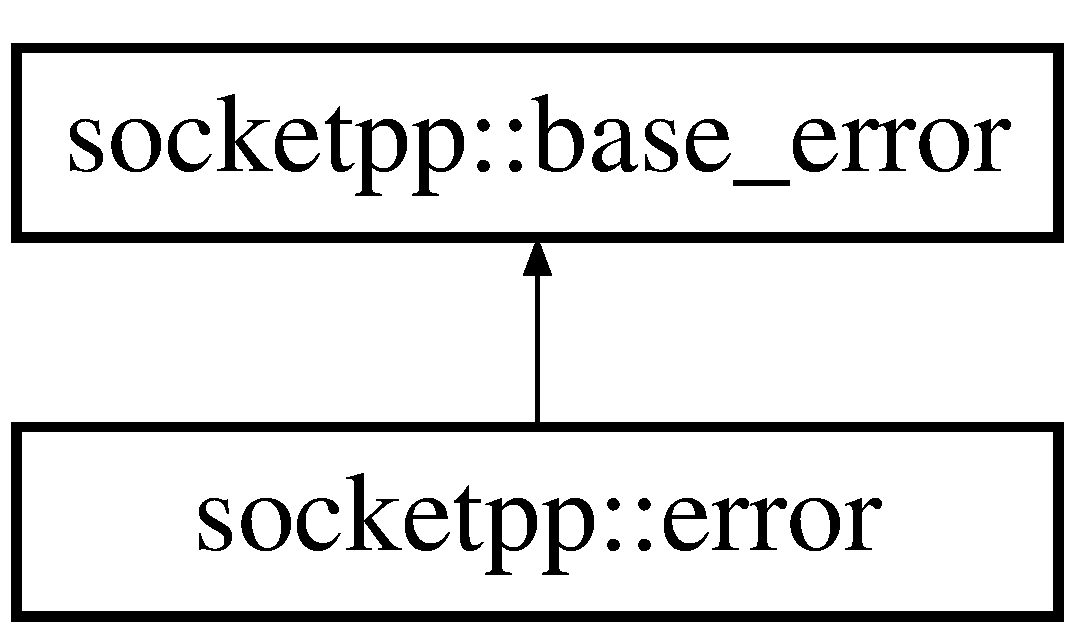
\includegraphics[height=2cm]{classsocketpp_1_1error}
\end{center}
\end{figure}
\subsection*{Public Member Functions}
\begin{CompactItemize}
\item 
\hyperlink{classsocketpp_1_1error_614fef9f326d7bb212771eb20a046290}{error} (const std::string \&meth, const std::string \&err, const std::string \&func=\char`\"{}\char`\"{})  throw ()
\item 
\hyperlink{classsocketpp_1_1error_1287e8ec1ff5f7b18d91ea65c2505ae8}{error} (const std::string \&meth, int err, const std::string \&func=\char`\"{}\char`\"{})  throw ()
\item 
int \hyperlink{classsocketpp_1_1error_e1d23816909f2663b5553d232110442b}{get\_\-errno} ()
\item 
\hyperlink{classsocketpp_1_1error_f41562a951322078eff6f56268f2f257}{$\sim$error} ()  throw ()
\end{CompactItemize}


\subsection{Constructor \& Destructor Documentation}
\hypertarget{classsocketpp_1_1error_614fef9f326d7bb212771eb20a046290}{
\index{socketpp::error@{socketpp::error}!error@{error}}
\index{error@{error}!socketpp::error@{socketpp::error}}
\subsubsection[{error}]{\setlength{\rightskip}{0pt plus 5cm}socketpp::error::error (const std::string \& {\em meth}, \/  const std::string \& {\em err}, \/  const std::string \& {\em func} = {\tt \char`\"{}\char`\"{}})  throw ()\hspace{0.3cm}{\tt  \mbox{[}inline\mbox{]}}}}
\label{classsocketpp_1_1error_614fef9f326d7bb212771eb20a046290}


\hypertarget{classsocketpp_1_1error_1287e8ec1ff5f7b18d91ea65c2505ae8}{
\index{socketpp::error@{socketpp::error}!error@{error}}
\index{error@{error}!socketpp::error@{socketpp::error}}
\subsubsection[{error}]{\setlength{\rightskip}{0pt plus 5cm}socketpp::error::error (const std::string \& {\em meth}, \/  int {\em err}, \/  const std::string \& {\em func} = {\tt \char`\"{}\char`\"{}})  throw ()\hspace{0.3cm}{\tt  \mbox{[}inline\mbox{]}}}}
\label{classsocketpp_1_1error_1287e8ec1ff5f7b18d91ea65c2505ae8}


\hypertarget{classsocketpp_1_1error_f41562a951322078eff6f56268f2f257}{
\index{socketpp::error@{socketpp::error}!$\sim$error@{$\sim$error}}
\index{$\sim$error@{$\sim$error}!socketpp::error@{socketpp::error}}
\subsubsection[{$\sim$error}]{\setlength{\rightskip}{0pt plus 5cm}socketpp::error::$\sim$error ()  throw ()\hspace{0.3cm}{\tt  \mbox{[}inline\mbox{]}}}}
\label{classsocketpp_1_1error_f41562a951322078eff6f56268f2f257}




\subsection{Member Function Documentation}
\hypertarget{classsocketpp_1_1error_e1d23816909f2663b5553d232110442b}{
\index{socketpp::error@{socketpp::error}!get\_\-errno@{get\_\-errno}}
\index{get\_\-errno@{get\_\-errno}!socketpp::error@{socketpp::error}}
\subsubsection[{get\_\-errno}]{\setlength{\rightskip}{0pt plus 5cm}int socketpp::error::get\_\-errno ()\hspace{0.3cm}{\tt  \mbox{[}inline\mbox{]}}}}
\label{classsocketpp_1_1error_e1d23816909f2663b5553d232110442b}




The documentation for this class was generated from the following file:\begin{CompactItemize}
\item 
\hyperlink{SockException_8h}{SockException.h}\end{CompactItemize}

\hypertarget{classftplib_1_1error__perm}{
\section{ftplib::error\_\-perm Class Reference}
\label{classftplib_1_1error__perm}\index{ftplib::error\_\-perm@{ftplib::error\_\-perm}}
}
{\tt \#include $<$ftp.h$>$}

Inheritance diagram for ftplib::error\_\-perm::\begin{figure}[H]
\begin{center}
\leavevmode
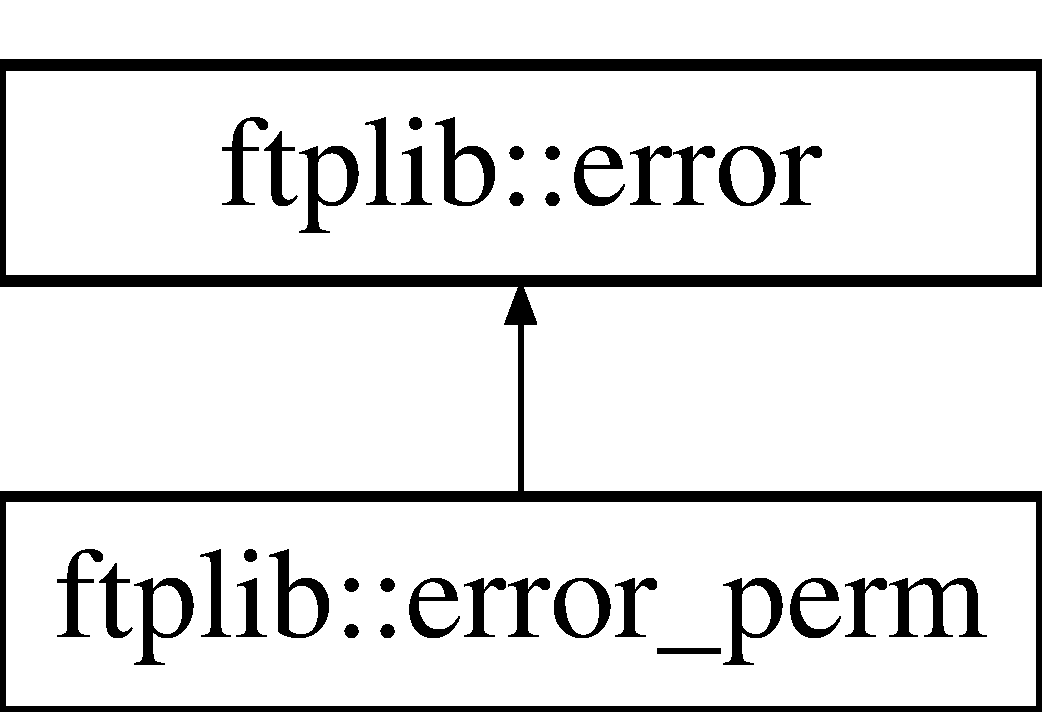
\includegraphics[height=2cm]{classftplib_1_1error__perm}
\end{center}
\end{figure}
\subsection*{Public Member Functions}
\begin{CompactItemize}
\item 
\hyperlink{classftplib_1_1error__perm_f39cb3638a78e6967e56d1f7e7346bfb}{error\_\-perm} (int code, const std::string \&msg)  throw ()
\item 
\hyperlink{classftplib_1_1error__perm_2d105a24ed475f01ed72bf1ce8f53fe8}{$\sim$error\_\-perm} ()  throw ()
\end{CompactItemize}


\subsection{Constructor \& Destructor Documentation}
\hypertarget{classftplib_1_1error__perm_f39cb3638a78e6967e56d1f7e7346bfb}{
\index{ftplib::error\_\-perm@{ftplib::error\_\-perm}!error\_\-perm@{error\_\-perm}}
\index{error\_\-perm@{error\_\-perm}!ftplib::error_perm@{ftplib::error\_\-perm}}
\subsubsection[{error\_\-perm}]{\setlength{\rightskip}{0pt plus 5cm}ftplib::error\_\-perm::error\_\-perm (int {\em code}, \/  const std::string \& {\em msg})  throw ()\hspace{0.3cm}{\tt  \mbox{[}inline\mbox{]}}}}
\label{classftplib_1_1error__perm_f39cb3638a78e6967e56d1f7e7346bfb}


\hypertarget{classftplib_1_1error__perm_2d105a24ed475f01ed72bf1ce8f53fe8}{
\index{ftplib::error\_\-perm@{ftplib::error\_\-perm}!$\sim$error\_\-perm@{$\sim$error\_\-perm}}
\index{$\sim$error\_\-perm@{$\sim$error\_\-perm}!ftplib::error_perm@{ftplib::error\_\-perm}}
\subsubsection[{$\sim$error\_\-perm}]{\setlength{\rightskip}{0pt plus 5cm}ftplib::error\_\-perm::$\sim$error\_\-perm ()  throw ()\hspace{0.3cm}{\tt  \mbox{[}inline\mbox{]}}}}
\label{classftplib_1_1error__perm_2d105a24ed475f01ed72bf1ce8f53fe8}




The documentation for this class was generated from the following file:\begin{CompactItemize}
\item 
\hyperlink{ftp_8h}{ftp.h}\end{CompactItemize}

\hypertarget{classftplib_1_1error__proto}{
\section{ftplib::error\_\-proto Class Reference}
\label{classftplib_1_1error__proto}\index{ftplib::error\_\-proto@{ftplib::error\_\-proto}}
}
exception thrown when a unexpected reply from the server is received  


{\tt \#include $<$ftp.h$>$}

\subsection*{Public Member Functions}
\begin{CompactItemize}
\item 
\hypertarget{classftplib_1_1error__proto_4d9a71a8162f838cb1cdd2997f64819b}{
\textbf{error\_\-proto} (const std::string \&msg)  throw ()}
\label{classftplib_1_1error__proto_4d9a71a8162f838cb1cdd2997f64819b}

\item 
\hypertarget{classftplib_1_1error__proto_67fb850475bc3becb1959822d0d6f470}{
virtual const char $\ast$ \textbf{what} () const   throw ()}
\label{classftplib_1_1error__proto_67fb850475bc3becb1959822d0d6f470}

\end{CompactItemize}


\subsection{Detailed Description}
exception thrown when a unexpected reply from the server is received 

The documentation for this class was generated from the following file:\begin{CompactItemize}
\item 
ftp.h\end{CompactItemize}

\hypertarget{classftplib_1_1error__temp}{
\section{ftplib::error\_\-temp Class Reference}
\label{classftplib_1_1error__temp}\index{ftplib::error\_\-temp@{ftplib::error\_\-temp}}
}
exception thrown when a \hyperlink{classftplib_1_1FTP}{FTP} error code in the range 400-499 is received  


{\tt \#include $<$ftp.h$>$}

Inheritance diagram for ftplib::error\_\-temp::\begin{figure}[H]
\begin{center}
\leavevmode
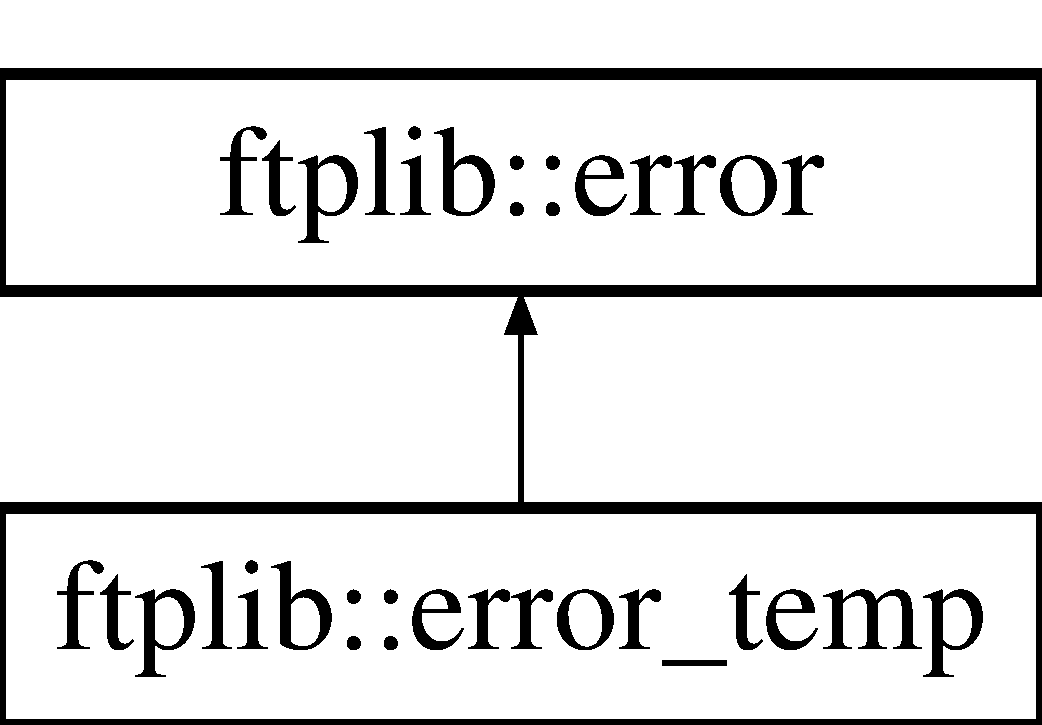
\includegraphics[height=2cm]{classftplib_1_1error__temp}
\end{center}
\end{figure}
\subsection*{Public Member Functions}
\begin{CompactItemize}
\item 
\hypertarget{classftplib_1_1error__temp_6c8a81fc949ee5591a85d5efeb492ea2}{
\textbf{error\_\-temp} (int code, const std::string \&msg)  throw ()}
\label{classftplib_1_1error__temp_6c8a81fc949ee5591a85d5efeb492ea2}

\end{CompactItemize}


\subsection{Detailed Description}
exception thrown when a \hyperlink{classftplib_1_1FTP}{FTP} error code in the range 400-499 is received 

The documentation for this class was generated from the following file:\begin{CompactItemize}
\item 
ftp.h\end{CompactItemize}

\hypertarget{classftplib_1_1FTP}{
\section{ftplib::FTP Class Reference}
\label{classftplib_1_1FTP}\index{ftplib::FTP@{ftplib::FTP}}
}
This class tries to imitate the \hyperlink{classftplib_1_1FTP}{ftplib.FTP} python class, with a few differences.  


{\tt \#include $<$ftp.h$>$}

\subsection*{Public Member Functions}
\begin{CompactItemize}
\item 
\hyperlink{classftplib_1_1FTP_178979abdc58593abdb31a882f370803}{FTP} (const std::string \&host=\char`\"{}\char`\"{}, const std::string \&user=\char`\"{}\char`\"{}, const std::string \&passwd=\char`\"{}\char`\"{}, double timeout=0.0)
\begin{CompactList}\small\item\em constructor \item\end{CompactList}\item 
std::string \hyperlink{classftplib_1_1FTP_fbd3444a33e5dd055474c9a0d6aabba5}{connect} (const std::string \&host, \hyperlink{namespacesocketpp_5517ef80f249b891a2ba64b95fc1e723}{socketpp::port\_\-t} port=21)
\begin{CompactList}\small\item\em connects to given \hyperlink{classftplib_1_1FTP}{FTP} server \item\end{CompactList}\item 
std::string \hyperlink{classftplib_1_1FTP_dc39751d00808d35183fb19c483b3589}{login} (const std::string \&user=\char`\"{}anonymous\char`\"{}, const std::string \&passwd=\char`\"{}\char`\"{})
\begin{CompactList}\small\item\em carries out the \hyperlink{classftplib_1_1FTP}{FTP} login \item\end{CompactList}\item 
std::string \hyperlink{classftplib_1_1FTP_5a876d670107df4b5924238450440eee}{sendcmd} (const std::string \&cmd)
\begin{CompactList}\small\item\em sends raw command and returns server response \item\end{CompactList}\item 
std::string \hyperlink{classftplib_1_1FTP_b04e374d4835e124959cee085df3fa4e}{retrlines} (const std::string \&cmd, std::ostream \&os=std::cout)
\begin{CompactList}\small\item\em Retrieve a file or directory listing in ASCII transfer mode. \item\end{CompactList}\item 
std::string \hyperlink{classftplib_1_1FTP_ad060fdb45fec7ccd5949e475df96982}{retrbinary} (const std::string \&cmd, std::ostream \&os)
\begin{CompactList}\small\item\em Retrieve a file in binary transfer mode. \item\end{CompactList}\item 
std::string \hyperlink{classftplib_1_1FTP_37c828c7d98c7da3fe3b936526118416}{storbinary} (const std::string \&cmd, std::istream \&is)
\begin{CompactList}\small\item\em Stor a file in binary transfer mode. \item\end{CompactList}\item 
std::string \hyperlink{classftplib_1_1FTP_956c5fa0546d7a6a2db0b4dee28f6868}{storlines} (const std::string \&cmd, std::istream \&is)
\begin{CompactList}\small\item\em Stor a file in ASCII transfer mode. \item\end{CompactList}\item 
std::vector$<$ std::string $>$ \hyperlink{classftplib_1_1FTP_a793fa113ee6fc82e3db3b7ed769ff3f}{nlst} (const std::string \&path=\char`\"{}.\char`\"{})
\begin{CompactList}\small\item\em obtains a std::vector containing existing file names in the passed path, through NLST command \item\end{CompactList}\item 
std::string \hyperlink{classftplib_1_1FTP_00e0a674ee47139d6205cd95cef42e73}{remove} (const std::string \&fname)
\begin{CompactList}\small\item\em remove a file from the server \item\end{CompactList}\item 
std::string \hyperlink{classftplib_1_1FTP_2a96ea655350a479cdf5f34254fd4ac8}{rmd} (const std::string \&dirname)
\begin{CompactList}\small\item\em remove a direcotry from the server \item\end{CompactList}\item 
std::string \hyperlink{classftplib_1_1FTP_05c4b118a0e278e70c79c1c42484f669}{mkd} (const std::string \&dirname)
\begin{CompactList}\small\item\em creates a new directory on the server \item\end{CompactList}\item 
std::string \hyperlink{classftplib_1_1FTP_0adece922028464ff064da24b539798d}{rename} (const std::string \&from, const std::string \&to)
\begin{CompactList}\small\item\em renames a file on the server \item\end{CompactList}\item 
std::string \hyperlink{classftplib_1_1FTP_7cd3c7fc71ae0c7dbdfcee88417d2685}{cwd} (const std::string \&path)
\begin{CompactList}\small\item\em changes working directory \item\end{CompactList}\item 
std::string \hyperlink{classftplib_1_1FTP_7c01c7b062848c7fc1d3caf95758b109}{pwd} ()
\begin{CompactList}\small\item\em returns current working directory \item\end{CompactList}\item 
std::string \hyperlink{classftplib_1_1FTP_42749c4425e33349f605ec0a8b389731}{dir} (const std::string \&path=\char`\"{}.\char`\"{}, std::ostream \&os=std::cout)
\begin{CompactList}\small\item\em lists all the files in the directory, through the LIST command param path directory to list, \char`\"{}.\char`\"{} if empty param os std::ostream on which output is written, std::cout if empty \item\end{CompactList}\item 
\hyperlink{classsocketpp_1_1Socket}{socketpp::Socket} \& \hyperlink{classftplib_1_1FTP_c949b3cd7b92534705ff041bb43d989b}{transfercmd} (const std::string \&cmd)
\begin{CompactList}\small\item\em initiate a transfer over the data connection, using PASV or PORT mode depending on previous calls to \hyperlink{classftplib_1_1FTP_e35230239f093f01fb295ccb007de1b2}{set\_\-pasv()} (default is PASV), and then send given command \item\end{CompactList}\item 
void \hyperlink{classftplib_1_1FTP_e35230239f093f01fb295ccb007de1b2}{set\_\-pasv} (bool p)  throw ()
\begin{CompactList}\small\item\em sets either PORT or PASV mode \item\end{CompactList}\item 
std::string \hyperlink{classftplib_1_1FTP_bd6e018a5cc17b1c8007064830823c71}{quit} ()
\begin{CompactList}\small\item\em sends the 'QUIT' command and closes socket \item\end{CompactList}\item 
void \hyperlink{classftplib_1_1FTP_4f36be9f23721435f19a7e5b1d702718}{close} ()
\begin{CompactList}\small\item\em closes socket \item\end{CompactList}\item 
void \hyperlink{classftplib_1_1FTP_a6603cda3b7c44c48c6a2b8d688d3bb7}{settimeout} (double time)
\begin{CompactList}\small\item\em sets timeout on all IO socket operations \item\end{CompactList}\end{CompactItemize}


\subsection{Detailed Description}
This class tries to imitate the \hyperlink{classftplib_1_1FTP}{ftplib.FTP} python class, with a few differences. 

\subsection{Constructor \& Destructor Documentation}
\hypertarget{classftplib_1_1FTP_178979abdc58593abdb31a882f370803}{
\index{ftplib::FTP@{ftplib::FTP}!FTP@{FTP}}
\index{FTP@{FTP}!ftplib::FTP@{ftplib::FTP}}
\subsubsection[{FTP}]{\setlength{\rightskip}{0pt plus 5cm}ftplib::FTP::FTP (const std::string \& {\em host} = {\tt \char`\"{}\char`\"{}}, \/  const std::string \& {\em user} = {\tt \char`\"{}\char`\"{}}, \/  const std::string \& {\em passwd} = {\tt \char`\"{}\char`\"{}}, \/  double {\em timeout} = {\tt 0.0})}}
\label{classftplib_1_1FTP_178979abdc58593abdb31a882f370803}


constructor 

\begin{Desc}
\item[Parameters:]
\begin{description}
\item[{\em host}]if not empty it connects to given hostname \item[{\em user}]if not empty it calls FTP::login(user, passw) \item[{\em passwd}]login password \item[{\em timeout}]if not empty it calls FTP::settimeout(timeout) \end{description}
\end{Desc}


\subsection{Member Function Documentation}
\hypertarget{classftplib_1_1FTP_4f36be9f23721435f19a7e5b1d702718}{
\index{ftplib::FTP@{ftplib::FTP}!close@{close}}
\index{close@{close}!ftplib::FTP@{ftplib::FTP}}
\subsubsection[{close}]{\setlength{\rightskip}{0pt plus 5cm}void ftplib::FTP::close ()}}
\label{classftplib_1_1FTP_4f36be9f23721435f19a7e5b1d702718}


closes socket 

\hypertarget{classftplib_1_1FTP_fbd3444a33e5dd055474c9a0d6aabba5}{
\index{ftplib::FTP@{ftplib::FTP}!connect@{connect}}
\index{connect@{connect}!ftplib::FTP@{ftplib::FTP}}
\subsubsection[{connect}]{\setlength{\rightskip}{0pt plus 5cm}std::string ftplib::FTP::connect (const std::string \& {\em host}, \/  {\bf socketpp::port\_\-t} {\em port} = {\tt 21})}}
\label{classftplib_1_1FTP_fbd3444a33e5dd055474c9a0d6aabba5}


connects to given \hyperlink{classftplib_1_1FTP}{FTP} server 

\begin{Desc}
\item[Parameters:]
\begin{description}
\item[{\em host}]remote server address \item[{\em port}]remote server port (21 if empty) \end{description}
\end{Desc}
\begin{Desc}
\item[Returns:]\hyperlink{classftplib_1_1FTP}{FTP} reply \end{Desc}
\hypertarget{classftplib_1_1FTP_7cd3c7fc71ae0c7dbdfcee88417d2685}{
\index{ftplib::FTP@{ftplib::FTP}!cwd@{cwd}}
\index{cwd@{cwd}!ftplib::FTP@{ftplib::FTP}}
\subsubsection[{cwd}]{\setlength{\rightskip}{0pt plus 5cm}std::string ftplib::FTP::cwd (const std::string \& {\em path})}}
\label{classftplib_1_1FTP_7cd3c7fc71ae0c7dbdfcee88417d2685}


changes working directory 

\begin{Desc}
\item[Parameters:]
\begin{description}
\item[{\em path}]directory name \end{description}
\end{Desc}
\begin{Desc}
\item[Returns:]\hyperlink{classftplib_1_1FTP}{FTP} reply \end{Desc}
\hypertarget{classftplib_1_1FTP_42749c4425e33349f605ec0a8b389731}{
\index{ftplib::FTP@{ftplib::FTP}!dir@{dir}}
\index{dir@{dir}!ftplib::FTP@{ftplib::FTP}}
\subsubsection[{dir}]{\setlength{\rightskip}{0pt plus 5cm}std::string ftplib::FTP::dir (const std::string \& {\em path} = {\tt \char`\"{}.\char`\"{}}, \/  std::ostream \& {\em os} = {\tt std::cout})}}
\label{classftplib_1_1FTP_42749c4425e33349f605ec0a8b389731}


lists all the files in the directory, through the LIST command param path directory to list, \char`\"{}.\char`\"{} if empty param os std::ostream on which output is written, std::cout if empty 

\begin{Desc}
\item[Returns:]\hyperlink{classftplib_1_1FTP}{FTP} reply \end{Desc}
\hypertarget{classftplib_1_1FTP_dc39751d00808d35183fb19c483b3589}{
\index{ftplib::FTP@{ftplib::FTP}!login@{login}}
\index{login@{login}!ftplib::FTP@{ftplib::FTP}}
\subsubsection[{login}]{\setlength{\rightskip}{0pt plus 5cm}std::string ftplib::FTP::login (const std::string \& {\em user} = {\tt \char`\"{}anonymous\char`\"{}}, \/  const std::string \& {\em passwd} = {\tt \char`\"{}\char`\"{}})}}
\label{classftplib_1_1FTP_dc39751d00808d35183fb19c483b3589}


carries out the \hyperlink{classftplib_1_1FTP}{FTP} login 

\begin{Desc}
\item[Parameters:]
\begin{description}
\item[{\em user}]username, \char`\"{}anonymous\char`\"{} if empty \item[{\em passwd}]password, if it's empty and user is \char`\"{}anonymous\char`\"{} it becomes \char`\"{}anonymous@\char`\"{} \end{description}
\end{Desc}
\begin{Desc}
\item[Returns:]\hyperlink{classftplib_1_1FTP}{FTP} reply \end{Desc}
\hypertarget{classftplib_1_1FTP_05c4b118a0e278e70c79c1c42484f669}{
\index{ftplib::FTP@{ftplib::FTP}!mkd@{mkd}}
\index{mkd@{mkd}!ftplib::FTP@{ftplib::FTP}}
\subsubsection[{mkd}]{\setlength{\rightskip}{0pt plus 5cm}std::string ftplib::FTP::mkd (const std::string \& {\em dirname})}}
\label{classftplib_1_1FTP_05c4b118a0e278e70c79c1c42484f669}


creates a new directory on the server 

\begin{Desc}
\item[Parameters:]
\begin{description}
\item[{\em dirname}]directory to remove \end{description}
\end{Desc}
\begin{Desc}
\item[Returns:]\hyperlink{classftplib_1_1FTP}{FTP} reply \end{Desc}
\hypertarget{classftplib_1_1FTP_a793fa113ee6fc82e3db3b7ed769ff3f}{
\index{ftplib::FTP@{ftplib::FTP}!nlst@{nlst}}
\index{nlst@{nlst}!ftplib::FTP@{ftplib::FTP}}
\subsubsection[{nlst}]{\setlength{\rightskip}{0pt plus 5cm}std::vector$<$ std::string $>$ ftplib::FTP::nlst (const std::string \& {\em path} = {\tt \char`\"{}.\char`\"{}})}}
\label{classftplib_1_1FTP_a793fa113ee6fc82e3db3b7ed769ff3f}


obtains a std::vector containing existing file names in the passed path, through NLST command 

\begin{Desc}
\item[Parameters:]
\begin{description}
\item[{\em path}]path to pass to NLST command, \char`\"{}.\char`\"{} if empty \end{description}
\end{Desc}
\begin{Desc}
\item[Returns:]file names vector \end{Desc}
\hypertarget{classftplib_1_1FTP_7c01c7b062848c7fc1d3caf95758b109}{
\index{ftplib::FTP@{ftplib::FTP}!pwd@{pwd}}
\index{pwd@{pwd}!ftplib::FTP@{ftplib::FTP}}
\subsubsection[{pwd}]{\setlength{\rightskip}{0pt plus 5cm}std::string ftplib::FTP::pwd ()}}
\label{classftplib_1_1FTP_7c01c7b062848c7fc1d3caf95758b109}


returns current working directory 

\begin{Desc}
\item[Returns:]current working directory \end{Desc}
\hypertarget{classftplib_1_1FTP_bd6e018a5cc17b1c8007064830823c71}{
\index{ftplib::FTP@{ftplib::FTP}!quit@{quit}}
\index{quit@{quit}!ftplib::FTP@{ftplib::FTP}}
\subsubsection[{quit}]{\setlength{\rightskip}{0pt plus 5cm}std::string ftplib::FTP::quit ()}}
\label{classftplib_1_1FTP_bd6e018a5cc17b1c8007064830823c71}


sends the 'QUIT' command and closes socket 

\begin{Desc}
\item[Returns:]\hyperlink{classftplib_1_1FTP}{FTP} reply \end{Desc}
\hypertarget{classftplib_1_1FTP_00e0a674ee47139d6205cd95cef42e73}{
\index{ftplib::FTP@{ftplib::FTP}!remove@{remove}}
\index{remove@{remove}!ftplib::FTP@{ftplib::FTP}}
\subsubsection[{remove}]{\setlength{\rightskip}{0pt plus 5cm}std::string ftplib::FTP::remove (const std::string \& {\em fname})}}
\label{classftplib_1_1FTP_00e0a674ee47139d6205cd95cef42e73}


remove a file from the server 

\begin{Desc}
\item[Parameters:]
\begin{description}
\item[{\em fname}]file to remove \end{description}
\end{Desc}
\begin{Desc}
\item[Returns:]\hyperlink{classftplib_1_1FTP}{FTP} reply \end{Desc}
\hypertarget{classftplib_1_1FTP_0adece922028464ff064da24b539798d}{
\index{ftplib::FTP@{ftplib::FTP}!rename@{rename}}
\index{rename@{rename}!ftplib::FTP@{ftplib::FTP}}
\subsubsection[{rename}]{\setlength{\rightskip}{0pt plus 5cm}std::string ftplib::FTP::rename (const std::string \& {\em from}, \/  const std::string \& {\em to})}}
\label{classftplib_1_1FTP_0adece922028464ff064da24b539798d}


renames a file on the server 

\begin{Desc}
\item[Parameters:]
\begin{description}
\item[{\em from}]file to rename \item[{\em to}]new file name \end{description}
\end{Desc}
\begin{Desc}
\item[Returns:]\hyperlink{classftplib_1_1FTP}{FTP} reply \end{Desc}
\hypertarget{classftplib_1_1FTP_ad060fdb45fec7ccd5949e475df96982}{
\index{ftplib::FTP@{ftplib::FTP}!retrbinary@{retrbinary}}
\index{retrbinary@{retrbinary}!ftplib::FTP@{ftplib::FTP}}
\subsubsection[{retrbinary}]{\setlength{\rightskip}{0pt plus 5cm}std::string ftplib::FTP::retrbinary (const std::string \& {\em cmd}, \/  std::ostream \& {\em os})}}
\label{classftplib_1_1FTP_ad060fdb45fec7ccd5949e475df96982}


Retrieve a file in binary transfer mode. 

\begin{Desc}
\item[Parameters:]
\begin{description}
\item[{\em cmd}]\hyperlink{classftplib_1_1FTP}{FTP} command, should be something like 'RETR filename' \item[{\em os}]std::ostream on which retrieved data are written \end{description}
\end{Desc}
\begin{Desc}
\item[Returns:]\hyperlink{classftplib_1_1FTP}{FTP} reply \end{Desc}
\hypertarget{classftplib_1_1FTP_b04e374d4835e124959cee085df3fa4e}{
\index{ftplib::FTP@{ftplib::FTP}!retrlines@{retrlines}}
\index{retrlines@{retrlines}!ftplib::FTP@{ftplib::FTP}}
\subsubsection[{retrlines}]{\setlength{\rightskip}{0pt plus 5cm}std::string ftplib::FTP::retrlines (const std::string \& {\em cmd}, \/  std::ostream \& {\em os} = {\tt std::cout})}}
\label{classftplib_1_1FTP_b04e374d4835e124959cee085df3fa4e}


Retrieve a file or directory listing in ASCII transfer mode. 

\begin{Desc}
\item[Parameters:]
\begin{description}
\item[{\em cmd}]\hyperlink{classftplib_1_1FTP}{FTP} command, should be something like RETR or LIST \item[{\em os}]std::ostream on which retrieved lines are written, std::cout if empty \end{description}
\end{Desc}
\begin{Desc}
\item[Returns:]\hyperlink{classftplib_1_1FTP}{FTP} reply \end{Desc}
\hypertarget{classftplib_1_1FTP_2a96ea655350a479cdf5f34254fd4ac8}{
\index{ftplib::FTP@{ftplib::FTP}!rmd@{rmd}}
\index{rmd@{rmd}!ftplib::FTP@{ftplib::FTP}}
\subsubsection[{rmd}]{\setlength{\rightskip}{0pt plus 5cm}std::string ftplib::FTP::rmd (const std::string \& {\em dirname})}}
\label{classftplib_1_1FTP_2a96ea655350a479cdf5f34254fd4ac8}


remove a direcotry from the server 

\begin{Desc}
\item[Parameters:]
\begin{description}
\item[{\em dirname}]directory to remove \end{description}
\end{Desc}
\begin{Desc}
\item[Returns:]\hyperlink{classftplib_1_1FTP}{FTP} reply \end{Desc}
\hypertarget{classftplib_1_1FTP_5a876d670107df4b5924238450440eee}{
\index{ftplib::FTP@{ftplib::FTP}!sendcmd@{sendcmd}}
\index{sendcmd@{sendcmd}!ftplib::FTP@{ftplib::FTP}}
\subsubsection[{sendcmd}]{\setlength{\rightskip}{0pt plus 5cm}std::string ftplib::FTP::sendcmd (const std::string \& {\em cmd})}}
\label{classftplib_1_1FTP_5a876d670107df4b5924238450440eee}


sends raw command and returns server response 

\begin{Desc}
\item[Parameters:]
\begin{description}
\item[{\em cmd}]\hyperlink{classftplib_1_1FTP}{FTP} command \end{description}
\end{Desc}
\begin{Desc}
\item[Returns:]\hyperlink{classftplib_1_1FTP}{FTP} reply \end{Desc}
\hypertarget{classftplib_1_1FTP_e35230239f093f01fb295ccb007de1b2}{
\index{ftplib::FTP@{ftplib::FTP}!set\_\-pasv@{set\_\-pasv}}
\index{set\_\-pasv@{set\_\-pasv}!ftplib::FTP@{ftplib::FTP}}
\subsubsection[{set\_\-pasv}]{\setlength{\rightskip}{0pt plus 5cm}void ftplib::FTP::set\_\-pasv (bool {\em p})  throw ()}}
\label{classftplib_1_1FTP_e35230239f093f01fb295ccb007de1b2}


sets either PORT or PASV mode 

\begin{Desc}
\item[Parameters:]
\begin{description}
\item[{\em p}]if true PASV, otherwise PORT \end{description}
\end{Desc}
\hypertarget{classftplib_1_1FTP_a6603cda3b7c44c48c6a2b8d688d3bb7}{
\index{ftplib::FTP@{ftplib::FTP}!settimeout@{settimeout}}
\index{settimeout@{settimeout}!ftplib::FTP@{ftplib::FTP}}
\subsubsection[{settimeout}]{\setlength{\rightskip}{0pt plus 5cm}void ftplib::FTP::settimeout (double {\em time})\hspace{0.3cm}{\tt  \mbox{[}inline\mbox{]}}}}
\label{classftplib_1_1FTP_a6603cda3b7c44c48c6a2b8d688d3bb7}


sets timeout on all IO socket operations 

\begin{Desc}
\item[Parameters:]
\begin{description}
\item[{\em time}]timeout value in seconds, if 0.0 timeout is cancelled \end{description}
\end{Desc}
\hypertarget{classftplib_1_1FTP_37c828c7d98c7da3fe3b936526118416}{
\index{ftplib::FTP@{ftplib::FTP}!storbinary@{storbinary}}
\index{storbinary@{storbinary}!ftplib::FTP@{ftplib::FTP}}
\subsubsection[{storbinary}]{\setlength{\rightskip}{0pt plus 5cm}std::string ftplib::FTP::storbinary (const std::string \& {\em cmd}, \/  std::istream \& {\em is})}}
\label{classftplib_1_1FTP_37c828c7d98c7da3fe3b936526118416}


Stor a file in binary transfer mode. 

\begin{Desc}
\item[Parameters:]
\begin{description}
\item[{\em cmd}]\hyperlink{classftplib_1_1FTP}{FTP} command, should be something like 'STOR filename' \item[{\em is}]std::istream from which data are red \end{description}
\end{Desc}
\begin{Desc}
\item[Returns:]\hyperlink{classftplib_1_1FTP}{FTP} reply \end{Desc}
\hypertarget{classftplib_1_1FTP_956c5fa0546d7a6a2db0b4dee28f6868}{
\index{ftplib::FTP@{ftplib::FTP}!storlines@{storlines}}
\index{storlines@{storlines}!ftplib::FTP@{ftplib::FTP}}
\subsubsection[{storlines}]{\setlength{\rightskip}{0pt plus 5cm}std::string ftplib::FTP::storlines (const std::string \& {\em cmd}, \/  std::istream \& {\em is})}}
\label{classftplib_1_1FTP_956c5fa0546d7a6a2db0b4dee28f6868}


Stor a file in ASCII transfer mode. 

\begin{Desc}
\item[Parameters:]
\begin{description}
\item[{\em cmd}]\hyperlink{classftplib_1_1FTP}{FTP} command, should be something like 'STOR filename' \item[{\em is}]std::istream from which data are red \end{description}
\end{Desc}
\begin{Desc}
\item[Returns:]\hyperlink{classftplib_1_1FTP}{FTP} reply \end{Desc}
\hypertarget{classftplib_1_1FTP_c949b3cd7b92534705ff041bb43d989b}{
\index{ftplib::FTP@{ftplib::FTP}!transfercmd@{transfercmd}}
\index{transfercmd@{transfercmd}!ftplib::FTP@{ftplib::FTP}}
\subsubsection[{transfercmd}]{\setlength{\rightskip}{0pt plus 5cm}{\bf socketpp::Socket} \& ftplib::FTP::transfercmd (const std::string \& {\em cmd})}}
\label{classftplib_1_1FTP_c949b3cd7b92534705ff041bb43d989b}


initiate a transfer over the data connection, using PASV or PORT mode depending on previous calls to \hyperlink{classftplib_1_1FTP_e35230239f093f01fb295ccb007de1b2}{set\_\-pasv()} (default is PASV), and then send given command 

\begin{Desc}
\item[Parameters:]
\begin{description}
\item[{\em cmd}]\hyperlink{classftplib_1_1FTP}{FTP} command to execute \end{description}
\end{Desc}
\begin{Desc}
\item[Returns:]connected FTP-data Socket object \end{Desc}


The documentation for this class was generated from the following files:\begin{CompactItemize}
\item 
\hyperlink{ftp_8h}{ftp.h}\item 
\hyperlink{ftp_8cpp}{ftp.cpp}\end{CompactItemize}

\hypertarget{classsocketpp_1_1gai__error}{
\section{socketpp::gai\_\-error Class Reference}
\label{classsocketpp_1_1gai__error}\index{socketpp::gai\_\-error@{socketpp::gai\_\-error}}
}
exception class related to C getaddrinfo() and getnameinfo() functions  


{\tt \#include $<$SockException.h$>$}

Inherits std::exception.

\subsection*{Public Member Functions}
\begin{CompactItemize}
\item 
\hyperlink{classsocketpp_1_1gai__error_617e195448875097f6561a39cca1f49b}{gai\_\-error} (const std::string \&meth, const std::string \&err, const std::string \&func=\char`\"{}\char`\"{})  throw ()
\item 
\hyperlink{classsocketpp_1_1gai__error_fc03a724180e0edd90f7502eedb68da1}{gai\_\-error} (const std::string \&meth, int err, const std::string \&func=\char`\"{}\char`\"{})  throw ()
\item 
\hypertarget{classsocketpp_1_1gai__error_1ee33e241f637684183e4c395a22a1df}{
virtual const char $\ast$ \hyperlink{classsocketpp_1_1gai__error_1ee33e241f637684183e4c395a22a1df}{what} () const   throw ()}
\label{classsocketpp_1_1gai__error_1ee33e241f637684183e4c395a22a1df}

\begin{CompactList}\small\item\em returns complete \hyperlink{classsocketpp_1_1error}{error} string \item\end{CompactList}\item 
\hypertarget{classsocketpp_1_1gai__error_efbf63e4224a250edc14f09bd15a1d3b}{
int \textbf{get\_\-gai\_\-errno} ()}
\label{classsocketpp_1_1gai__error_efbf63e4224a250edc14f09bd15a1d3b}

\end{CompactItemize}


\subsection{Detailed Description}
exception class related to C getaddrinfo() and getnameinfo() functions 

\subsection{Constructor \& Destructor Documentation}
\hypertarget{classsocketpp_1_1gai__error_617e195448875097f6561a39cca1f49b}{
\index{socketpp::gai\_\-error@{socketpp::gai\_\-error}!gai\_\-error@{gai\_\-error}}
\index{gai\_\-error@{gai\_\-error}!socketpp::gai_error@{socketpp::gai\_\-error}}
\subsubsection[{gai\_\-error}]{\setlength{\rightskip}{0pt plus 5cm}socketpp::gai\_\-error::gai\_\-error (const std::string \& {\em meth}, \/  const std::string \& {\em err}, \/  const std::string \& {\em func} = {\tt \char`\"{}\char`\"{}})  throw ()\hspace{0.3cm}{\tt  \mbox{[}inline\mbox{]}}}}
\label{classsocketpp_1_1gai__error_617e195448875097f6561a39cca1f49b}


\begin{Desc}
\item[Parameters:]
\begin{description}
\item[{\em meth}]method which threw exception \item[{\em err}]\hyperlink{classsocketpp_1_1error}{error} description string \item[{\em func}]C function which returned \hyperlink{classsocketpp_1_1error}{error} \end{description}
\end{Desc}
\hypertarget{classsocketpp_1_1gai__error_fc03a724180e0edd90f7502eedb68da1}{
\index{socketpp::gai\_\-error@{socketpp::gai\_\-error}!gai\_\-error@{gai\_\-error}}
\index{gai\_\-error@{gai\_\-error}!socketpp::gai_error@{socketpp::gai\_\-error}}
\subsubsection[{gai\_\-error}]{\setlength{\rightskip}{0pt plus 5cm}socketpp::gai\_\-error::gai\_\-error (const std::string \& {\em meth}, \/  int {\em err}, \/  const std::string \& {\em func} = {\tt \char`\"{}\char`\"{}})  throw ()\hspace{0.3cm}{\tt  \mbox{[}inline\mbox{]}}}}
\label{classsocketpp_1_1gai__error_fc03a724180e0edd90f7502eedb68da1}


\begin{Desc}
\item[Parameters:]
\begin{description}
\item[{\em meth}]method which threw exception \item[{\em err}]h\_\-errno code \item[{\em func}]C function which returned \hyperlink{classsocketpp_1_1error}{error} \end{description}
\end{Desc}


The documentation for this class was generated from the following file:\begin{CompactItemize}
\item 
SockException.h\end{CompactItemize}

\hypertarget{classsocketpp_1_1h__error}{
\section{socketpp::h\_\-error Class Reference}
\label{classsocketpp_1_1h__error}\index{socketpp::h\_\-error@{socketpp::h\_\-error}}
}
address-related exception class  


{\tt \#include $<$SockException.h$>$}

Inherits std::exception.

\subsection*{Public Member Functions}
\begin{CompactItemize}
\item 
\hyperlink{classsocketpp_1_1h__error_c15a1c6216114250241349fdfcdeb98a}{h\_\-error} (const std::string \&meth, const std::string \&err, const std::string \&func=\char`\"{}\char`\"{})  throw ()
\item 
\hypertarget{classsocketpp_1_1h__error_055c1a5b55b5d02fe81fd74cb8b900d2}{
virtual const char $\ast$ \hyperlink{classsocketpp_1_1h__error_055c1a5b55b5d02fe81fd74cb8b900d2}{what} () const   throw ()}
\label{classsocketpp_1_1h__error_055c1a5b55b5d02fe81fd74cb8b900d2}

\begin{CompactList}\small\item\em returns complete \hyperlink{classsocketpp_1_1error}{error} string \item\end{CompactList}\end{CompactItemize}


\subsection{Detailed Description}
address-related exception class 

\subsection{Constructor \& Destructor Documentation}
\hypertarget{classsocketpp_1_1h__error_c15a1c6216114250241349fdfcdeb98a}{
\index{socketpp::h\_\-error@{socketpp::h\_\-error}!h\_\-error@{h\_\-error}}
\index{h\_\-error@{h\_\-error}!socketpp::h_error@{socketpp::h\_\-error}}
\subsubsection[{h\_\-error}]{\setlength{\rightskip}{0pt plus 5cm}socketpp::h\_\-error::h\_\-error (const std::string \& {\em meth}, \/  const std::string \& {\em err}, \/  const std::string \& {\em func} = {\tt \char`\"{}\char`\"{}})  throw ()\hspace{0.3cm}{\tt  \mbox{[}inline\mbox{]}}}}
\label{classsocketpp_1_1h__error_c15a1c6216114250241349fdfcdeb98a}


\begin{Desc}
\item[Parameters:]
\begin{description}
\item[{\em meth}]method which threw exception \item[{\em err}]\hyperlink{classsocketpp_1_1error}{error} description string \item[{\em func}]C function which returned \hyperlink{classsocketpp_1_1error}{error} \end{description}
\end{Desc}


The documentation for this class was generated from the following file:\begin{CompactItemize}
\item 
SockException.h\end{CompactItemize}

\hypertarget{classsocketpp_1_1ICMP__IP__RawSocket}{
\section{socketpp::ICMP\_\-IP\_\-RawSocket Class Reference}
\label{classsocketpp_1_1ICMP__IP__RawSocket}\index{socketpp::ICMP\_\-IP\_\-RawSocket@{socketpp::ICMP\_\-IP\_\-RawSocket}}
}
ICMP raw socket with IP header handling.  


{\tt \#include $<$RawSocket.h$>$}

Inheritance diagram for socketpp::ICMP\_\-IP\_\-RawSocket::\begin{figure}[H]
\begin{center}
\leavevmode
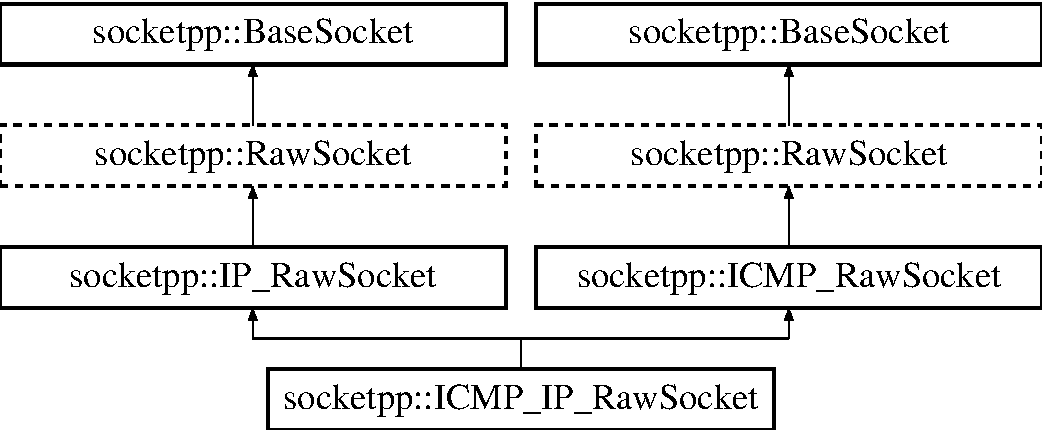
\includegraphics[height=4cm]{classsocketpp_1_1ICMP__IP__RawSocket}
\end{center}
\end{figure}
\subsection*{Public Member Functions}
\begin{CompactItemize}
\item 
\hypertarget{classsocketpp_1_1ICMP__IP__RawSocket_c94fd53fce785a8b9ac5e53c8b1fb694}{
\hyperlink{classsocketpp_1_1ICMP__IP__RawSocket_c94fd53fce785a8b9ac5e53c8b1fb694}{ICMP\_\-IP\_\-RawSocket} ()}
\label{classsocketpp_1_1ICMP__IP__RawSocket_c94fd53fce785a8b9ac5e53c8b1fb694}

\begin{CompactList}\small\item\em constructor which calls RawSocket(ipproto\_\-udp) and setsockopt(ip\_\-hdrincl) \item\end{CompactList}\item 
\hypertarget{classsocketpp_1_1ICMP__IP__RawSocket_08d5813e94daff127499b2d1f7e93324}{
void \hyperlink{classsocketpp_1_1ICMP__IP__RawSocket_08d5813e94daff127499b2d1f7e93324}{build\_\-IP\_\-header} (\_\-u32 saddr, \_\-u32 daddr, \_\-u8 ttl=64, \_\-u8 version=4, \_\-u8 protocol=IPPROTO\_\-ICMP, \_\-u16 id=0, \_\-u8 tos=0, \_\-u16 frag\_\-off=0, \_\-u8 ihl=0, \_\-u16 tot\_\-len=0, \_\-u16 check=0)}
\label{classsocketpp_1_1ICMP__IP__RawSocket_08d5813e94daff127499b2d1f7e93324}

\begin{CompactList}\small\item\em builds the internal IP header to send \item\end{CompactList}\item 
\hypertarget{classsocketpp_1_1ICMP__IP__RawSocket_c3f54f7a266586af46e4bfa4494f90d6}{
void \hyperlink{classsocketpp_1_1ICMP__IP__RawSocket_c3f54f7a266586af46e4bfa4494f90d6}{adjust\_\-ICMP\_\-IP\_\-all} ()}
\label{classsocketpp_1_1ICMP__IP__RawSocket_c3f54f7a266586af46e4bfa4494f90d6}

\begin{CompactList}\small\item\em calls adjust\_\-ICMP\_\-all() \&\& \hyperlink{classsocketpp_1_1IP__RawSocket_45e60510233daaa2f279d3a4706fdce5}{adjust\_\-IP\_\-all()} \item\end{CompactList}\end{CompactItemize}
\subsection*{Protected Member Functions}
\begin{CompactItemize}
\item 
\hypertarget{classsocketpp_1_1ICMP__IP__RawSocket_49a62078d6febf7a11b9350de1e23903}{
void \textbf{\_\-build\_\-packet} (std::string \&packet)}
\label{classsocketpp_1_1ICMP__IP__RawSocket_49a62078d6febf7a11b9350de1e23903}

\item 
\hypertarget{classsocketpp_1_1ICMP__IP__RawSocket_6d2f188d46030afa13f9c3971d43d518}{
void \textbf{\_\-set\_\-fields} (const std::string \&packet)}
\label{classsocketpp_1_1ICMP__IP__RawSocket_6d2f188d46030afa13f9c3971d43d518}

\end{CompactItemize}


\subsection{Detailed Description}
ICMP raw socket with IP header handling. 

The documentation for this class was generated from the following files:\begin{CompactItemize}
\item 
RawSocket.h\item 
RawSocket.cpp\end{CompactItemize}

\hypertarget{classsocketpp_1_1ICMP__RawSocket}{
\section{socketpp::ICMP\_\-RawSocket Class Reference}
\label{classsocketpp_1_1ICMP__RawSocket}\index{socketpp::ICMP\_\-RawSocket@{socketpp::ICMP\_\-RawSocket}}
}
ICMP raw socket without IP header handling.  


{\tt \#include $<$RawSocket.h$>$}

Inheritance diagram for socketpp::ICMP\_\-RawSocket::\begin{figure}[H]
\begin{center}
\leavevmode
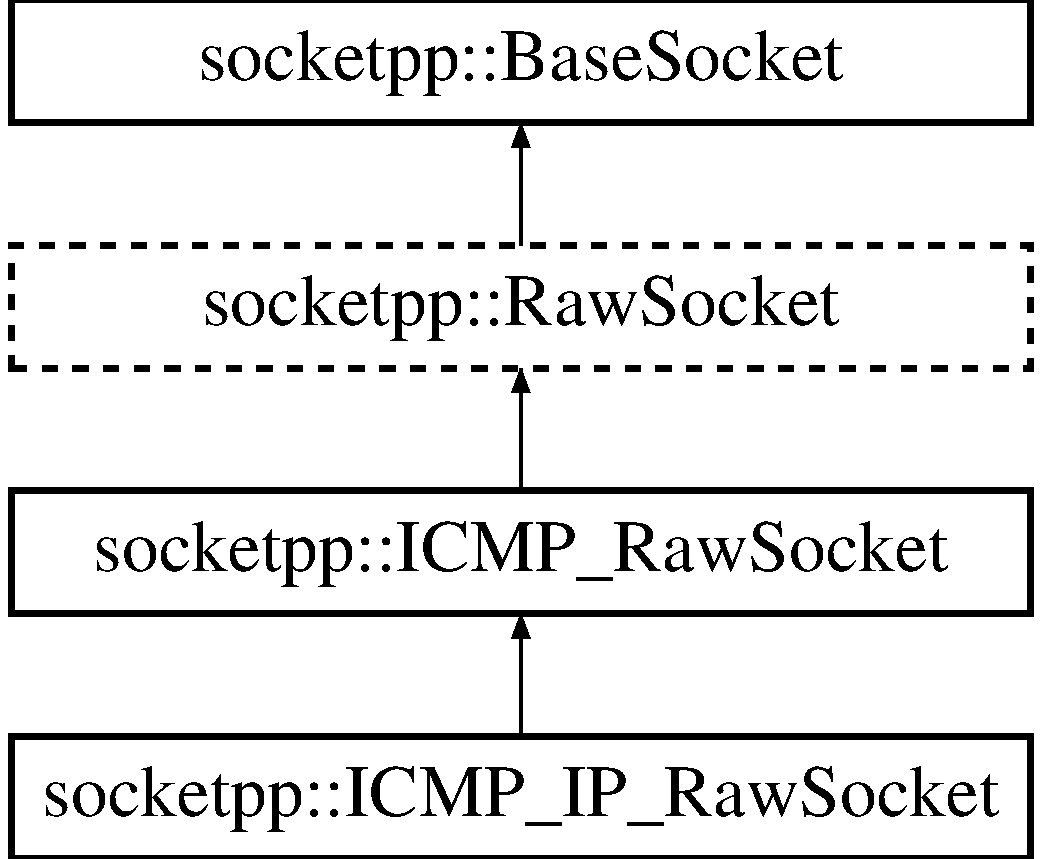
\includegraphics[height=4cm]{classsocketpp_1_1ICMP__RawSocket}
\end{center}
\end{figure}
\subsection*{Public Member Functions}
\begin{CompactItemize}
\item 
\hypertarget{classsocketpp_1_1ICMP__RawSocket_bed3b5ca33a0f7b4be42a9e6167266c0}{
\hyperlink{classsocketpp_1_1ICMP__RawSocket_bed3b5ca33a0f7b4be42a9e6167266c0}{ICMP\_\-RawSocket} ()}
\label{classsocketpp_1_1ICMP__RawSocket_bed3b5ca33a0f7b4be42a9e6167266c0}

\begin{CompactList}\small\item\em constructor which calls RawSocket(ipproto\_\-icmp) \item\end{CompactList}\item 
void \hyperlink{classsocketpp_1_1ICMP__RawSocket_7d8d54d4771f4012246835819421fbeb}{build\_\-ICMP\_\-header} (const icmphdr \&icmp)
\begin{CompactList}\small\item\em builds the internal ICMP header to send \item\end{CompactList}\item 
\hypertarget{classsocketpp_1_1ICMP__RawSocket_21c279a1c1a31d2395b2930de49b9c02}{
void \hyperlink{classsocketpp_1_1ICMP__RawSocket_21c279a1c1a31d2395b2930de49b9c02}{build\_\-ICMP\_\-header} (\_\-u8 type, \_\-u8 code=0, \_\-u16 id=0, \_\-u16 sequence=0, \_\-u16 check=0)}
\label{classsocketpp_1_1ICMP__RawSocket_21c279a1c1a31d2395b2930de49b9c02}

\begin{CompactList}\small\item\em builds the internal ICMP header to send \item\end{CompactList}\item 
\hypertarget{classsocketpp_1_1ICMP__RawSocket_ab00bba6ed9fe98ca771fc3310983c97}{
void \hyperlink{classsocketpp_1_1ICMP__RawSocket_ab00bba6ed9fe98ca771fc3310983c97}{adjust\_\-ICMP\_\-csum} ()}
\label{classsocketpp_1_1ICMP__RawSocket_ab00bba6ed9fe98ca771fc3310983c97}

\begin{CompactList}\small\item\em sets the internal ICMP header checksum \item\end{CompactList}\item 
void \hyperlink{classsocketpp_1_1ICMP__RawSocket_9b0ed9bb87d2895f2302db13b7ca5f06}{get\_\-ICMP\_\-header} (icmphdr \&icmp)
\begin{CompactList}\small\item\em gets the received ICMP header \item\end{CompactList}\end{CompactItemize}
\subsection*{Static Public Member Functions}
\begin{CompactItemize}
\item 
static \_\-u16 \hyperlink{classsocketpp_1_1ICMP__RawSocket_6c8a1364919485932221942c472ea95e}{icmp\_\-checksum} (const struct icmphdr \&icmp, const void $\ast$payload=NULL, size\_\-t psize=0)
\begin{CompactList}\small\item\em calculates ICMP header checksum \item\end{CompactList}\item 
static \_\-u16 \hyperlink{classsocketpp_1_1ICMP__RawSocket_eb8e83796aefe5a5dd7035490902a537}{icmp\_\-checksum} (const struct icmphdr \&icmp, const std::string \&payload)
\begin{CompactList}\small\item\em calculates ICMP header checksum \item\end{CompactList}\end{CompactItemize}
\subsection*{Protected Member Functions}
\begin{CompactItemize}
\item 
\hypertarget{classsocketpp_1_1ICMP__RawSocket_1dcbe47b02ddfff9545cedca9d78e36c}{
virtual void \textbf{\_\-build\_\-packet} (std::string \&packet) const }
\label{classsocketpp_1_1ICMP__RawSocket_1dcbe47b02ddfff9545cedca9d78e36c}

\item 
\hypertarget{classsocketpp_1_1ICMP__RawSocket_e183b11c080f5d74dbc386ec53e7feb5}{
virtual void \textbf{\_\-set\_\-fields} (const std::string \&packet)}
\label{classsocketpp_1_1ICMP__RawSocket_e183b11c080f5d74dbc386ec53e7feb5}

\end{CompactItemize}
\subsection*{Static Protected Member Functions}
\begin{CompactItemize}
\item 
\hypertarget{classsocketpp_1_1ICMP__RawSocket_9ecff00c5732fced1d5dda68a5709651}{
static void \textbf{\_\-icmp\_\-convert} (const struct icmphdr \&, struct icmphdr \&)}
\label{classsocketpp_1_1ICMP__RawSocket_9ecff00c5732fced1d5dda68a5709651}

\end{CompactItemize}
\subsection*{Protected Attributes}
\begin{CompactItemize}
\item 
\hypertarget{classsocketpp_1_1ICMP__RawSocket_31f1ab3a8beaf8d4cb5b192e644e3f33}{
icmphdr \textbf{ICMP\_\-h}}
\label{classsocketpp_1_1ICMP__RawSocket_31f1ab3a8beaf8d4cb5b192e644e3f33}

\item 
\hypertarget{classsocketpp_1_1ICMP__RawSocket_1304716643ef2274b8c1c195359110c6}{
icmphdr \textbf{rcvd\_\-ICMP\_\-h}}
\label{classsocketpp_1_1ICMP__RawSocket_1304716643ef2274b8c1c195359110c6}

\end{CompactItemize}


\subsection{Detailed Description}
ICMP raw socket without IP header handling. 

\subsection{Member Function Documentation}
\hypertarget{classsocketpp_1_1ICMP__RawSocket_7d8d54d4771f4012246835819421fbeb}{
\index{socketpp::ICMP\_\-RawSocket@{socketpp::ICMP\_\-RawSocket}!build\_\-ICMP\_\-header@{build\_\-ICMP\_\-header}}
\index{build\_\-ICMP\_\-header@{build\_\-ICMP\_\-header}!socketpp::ICMP_RawSocket@{socketpp::ICMP\_\-RawSocket}}
\subsubsection[{build\_\-ICMP\_\-header}]{\setlength{\rightskip}{0pt plus 5cm}void socketpp::ICMP\_\-RawSocket::build\_\-ICMP\_\-header (const icmphdr \& {\em icmp})}}
\label{classsocketpp_1_1ICMP__RawSocket_7d8d54d4771f4012246835819421fbeb}


builds the internal ICMP header to send 

\begin{Desc}
\item[Parameters:]
\begin{description}
\item[{\em icmp}]icmp header \end{description}
\end{Desc}
\hypertarget{classsocketpp_1_1ICMP__RawSocket_9b0ed9bb87d2895f2302db13b7ca5f06}{
\index{socketpp::ICMP\_\-RawSocket@{socketpp::ICMP\_\-RawSocket}!get\_\-ICMP\_\-header@{get\_\-ICMP\_\-header}}
\index{get\_\-ICMP\_\-header@{get\_\-ICMP\_\-header}!socketpp::ICMP_RawSocket@{socketpp::ICMP\_\-RawSocket}}
\subsubsection[{get\_\-ICMP\_\-header}]{\setlength{\rightskip}{0pt plus 5cm}void socketpp::ICMP\_\-RawSocket::get\_\-ICMP\_\-header (icmphdr \& {\em icmp})}}
\label{classsocketpp_1_1ICMP__RawSocket_9b0ed9bb87d2895f2302db13b7ca5f06}


gets the received ICMP header 

\begin{Desc}
\item[Parameters:]
\begin{description}
\item[{\em icmp}]ICMP header to modify \end{description}
\end{Desc}
\hypertarget{classsocketpp_1_1ICMP__RawSocket_eb8e83796aefe5a5dd7035490902a537}{
\index{socketpp::ICMP\_\-RawSocket@{socketpp::ICMP\_\-RawSocket}!icmp\_\-checksum@{icmp\_\-checksum}}
\index{icmp\_\-checksum@{icmp\_\-checksum}!socketpp::ICMP_RawSocket@{socketpp::ICMP\_\-RawSocket}}
\subsubsection[{icmp\_\-checksum}]{\setlength{\rightskip}{0pt plus 5cm}\_\-u16 socketpp::ICMP\_\-RawSocket::icmp\_\-checksum (const struct icmphdr \& {\em icmp}, \/  const std::string \& {\em payload})\hspace{0.3cm}{\tt  \mbox{[}static\mbox{]}}}}
\label{classsocketpp_1_1ICMP__RawSocket_eb8e83796aefe5a5dd7035490902a537}


calculates ICMP header checksum 

\begin{Desc}
\item[Parameters:]
\begin{description}
\item[{\em icmp}]ICMP header \item[{\em payload}]data payload field \end{description}
\end{Desc}
\begin{Desc}
\item[Returns:]checksum value \end{Desc}
\hypertarget{classsocketpp_1_1ICMP__RawSocket_6c8a1364919485932221942c472ea95e}{
\index{socketpp::ICMP\_\-RawSocket@{socketpp::ICMP\_\-RawSocket}!icmp\_\-checksum@{icmp\_\-checksum}}
\index{icmp\_\-checksum@{icmp\_\-checksum}!socketpp::ICMP_RawSocket@{socketpp::ICMP\_\-RawSocket}}
\subsubsection[{icmp\_\-checksum}]{\setlength{\rightskip}{0pt plus 5cm}\_\-u16 socketpp::ICMP\_\-RawSocket::icmp\_\-checksum (const struct icmphdr \& {\em icmp}, \/  const void $\ast$ {\em payload} = {\tt NULL}, \/  size\_\-t {\em psize} = {\tt 0})\hspace{0.3cm}{\tt  \mbox{[}static\mbox{]}}}}
\label{classsocketpp_1_1ICMP__RawSocket_6c8a1364919485932221942c472ea95e}


calculates ICMP header checksum 

\begin{Desc}
\item[Parameters:]
\begin{description}
\item[{\em icmp}]ICMP header \item[{\em payload}]pointer to data payload field \item[{\em psize}]data payload size \end{description}
\end{Desc}
\begin{Desc}
\item[Returns:]checksum value \end{Desc}


The documentation for this class was generated from the following files:\begin{CompactItemize}
\item 
RawSocket.h\item 
RawSocket.cpp\end{CompactItemize}

\hypertarget{classsocketpp_1_1IP__RawSocket}{
\section{socketpp::IP\_\-RawSocket Class Reference}
\label{classsocketpp_1_1IP__RawSocket}\index{socketpp::IP\_\-RawSocket@{socketpp::IP\_\-RawSocket}}
}
IP raw socket, without transport-based protocol. ONLY SENDING METHODS WORK.  


{\tt \#include $<$RawSocket.h$>$}

Inheritance diagram for socketpp::IP\_\-RawSocket::\begin{figure}[H]
\begin{center}
\leavevmode
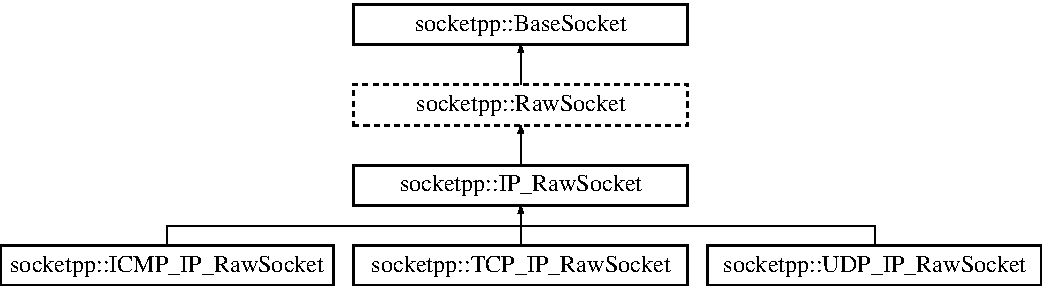
\includegraphics[height=3.8488cm]{classsocketpp_1_1IP__RawSocket}
\end{center}
\end{figure}
\subsection*{Public Member Functions}
\begin{CompactItemize}
\item 
\hypertarget{classsocketpp_1_1IP__RawSocket_e523748e7ca5bbcf7b74d804d356630e}{
\hyperlink{classsocketpp_1_1IP__RawSocket_e523748e7ca5bbcf7b74d804d356630e}{IP\_\-RawSocket} ()}
\label{classsocketpp_1_1IP__RawSocket_e523748e7ca5bbcf7b74d804d356630e}

\begin{CompactList}\small\item\em constructor which calls RawSocket(ipproto\_\-raw) \item\end{CompactList}\item 
void \hyperlink{classsocketpp_1_1IP__RawSocket_f93c51a7a8284fe9d2b24019b13a5803}{build\_\-IP\_\-header} (const iphdr \&ip)
\begin{CompactList}\small\item\em builds the internal IP header to send \item\end{CompactList}\item 
\hypertarget{classsocketpp_1_1IP__RawSocket_64e10d0fc07e687ebfeeeff45f29533e}{
virtual void \hyperlink{classsocketpp_1_1IP__RawSocket_64e10d0fc07e687ebfeeeff45f29533e}{build\_\-IP\_\-header} (\_\-u32 saddr, \_\-u32 daddr, \_\-u8 ttl=64, \_\-u8 version=4, \_\-u8 protocol=0, \_\-u16 id=0, \_\-u8 tos=0, \_\-u16 frag\_\-off=0, \_\-u8 ihl=0, \_\-u16 tot\_\-len=0, \_\-u16 check=0)}
\label{classsocketpp_1_1IP__RawSocket_64e10d0fc07e687ebfeeeff45f29533e}

\begin{CompactList}\small\item\em builds the internal IP header to send \item\end{CompactList}\item 
void \hyperlink{classsocketpp_1_1IP__RawSocket_82c0b2c75d081bc84d8e60bf18199e65}{set\_\-IP\_\-options} (const char $\ast$opt, size\_\-t len)
\begin{CompactList}\small\item\em sets the IP options field \item\end{CompactList}\item 
void \hyperlink{classsocketpp_1_1IP__RawSocket_9d88ecec5e362b3cf3d3dbc51d5dd0cd}{set\_\-IP\_\-options} (const std::string \&opt)
\begin{CompactList}\small\item\em sets the IP options field \item\end{CompactList}\item 
\hypertarget{classsocketpp_1_1IP__RawSocket_187bab79c6a8bae17b400a132063a9d1}{
virtual void \hyperlink{classsocketpp_1_1IP__RawSocket_187bab79c6a8bae17b400a132063a9d1}{adjust\_\-IP\_\-csum} ()}
\label{classsocketpp_1_1IP__RawSocket_187bab79c6a8bae17b400a132063a9d1}

\begin{CompactList}\small\item\em sets IP checksum field \item\end{CompactList}\item 
\hypertarget{classsocketpp_1_1IP__RawSocket_32d2c08139fb43abb92679bdabecf778}{
virtual void \hyperlink{classsocketpp_1_1IP__RawSocket_32d2c08139fb43abb92679bdabecf778}{adjust\_\-IP\_\-tot\_\-len} ()}
\label{classsocketpp_1_1IP__RawSocket_32d2c08139fb43abb92679bdabecf778}

\begin{CompactList}\small\item\em sets IP \char`\"{}total length\char`\"{} field \item\end{CompactList}\item 
\hypertarget{classsocketpp_1_1IP__RawSocket_d84d5e193a15baf421c64011a9c27359}{
void \hyperlink{classsocketpp_1_1IP__RawSocket_d84d5e193a15baf421c64011a9c27359}{adjust\_\-IP\_\-ihl} ()}
\label{classsocketpp_1_1IP__RawSocket_d84d5e193a15baf421c64011a9c27359}

\begin{CompactList}\small\item\em sets IP \char`\"{}header length\char`\"{} field \item\end{CompactList}\item 
\hypertarget{classsocketpp_1_1IP__RawSocket_45e60510233daaa2f279d3a4706fdce5}{
void \hyperlink{classsocketpp_1_1IP__RawSocket_45e60510233daaa2f279d3a4706fdce5}{adjust\_\-IP\_\-all} ()}
\label{classsocketpp_1_1IP__RawSocket_45e60510233daaa2f279d3a4706fdce5}

\begin{CompactList}\small\item\em calls \hyperlink{classsocketpp_1_1IP__RawSocket_32d2c08139fb43abb92679bdabecf778}{adjust\_\-IP\_\-tot\_\-len()} \&\& \hyperlink{classsocketpp_1_1IP__RawSocket_d84d5e193a15baf421c64011a9c27359}{adjust\_\-IP\_\-ihl()} \&\& \hyperlink{classsocketpp_1_1IP__RawSocket_187bab79c6a8bae17b400a132063a9d1}{adjust\_\-IP\_\-csum()} \item\end{CompactList}\item 
void \hyperlink{classsocketpp_1_1IP__RawSocket_e477f483d5a8baa76c60399d0809d043}{get\_\-IP\_\-header} (iphdr \&ip)
\begin{CompactList}\small\item\em gets received IP header \item\end{CompactList}\item 
size\_\-t \hyperlink{classsocketpp_1_1IP__RawSocket_686fcc72997b0843b2ece0c4d8a5735d}{get\_\-IP\_\-options} (char $\ast$opt, size\_\-t len)
\begin{CompactList}\small\item\em gets received IP options \item\end{CompactList}\item 
size\_\-t \hyperlink{classsocketpp_1_1IP__RawSocket_c9bec0c1db60871bb1cb5560b97e02ed}{get\_\-IP\_\-options} (std::string \&opt)
\begin{CompactList}\small\item\em gets received IP options \item\end{CompactList}\end{CompactItemize}
\subsection*{Static Public Member Functions}
\begin{CompactItemize}
\item 
\hypertarget{classsocketpp_1_1IP__RawSocket_91cc7b27ebb5eb8da6be6cdd14087f21}{
static \_\-u16 \textbf{ip\_\-checksum} (const struct iphdr \&ip, const void $\ast$payload=NULL, size\_\-t psize=0, const void $\ast$ip\_\-opt=NULL, size\_\-t ip\_\-opt\_\-len=0)}
\label{classsocketpp_1_1IP__RawSocket_91cc7b27ebb5eb8da6be6cdd14087f21}

\item 
\hypertarget{classsocketpp_1_1IP__RawSocket_6b48548362fb5509bbba7d36e9ffdb5d}{
static \_\-u16 \textbf{ip\_\-checksum} (const struct iphdr \&ip, const std::string \&payload, const std::string \&ip\_\-opt)}
\label{classsocketpp_1_1IP__RawSocket_6b48548362fb5509bbba7d36e9ffdb5d}

\end{CompactItemize}
\subsection*{Protected Member Functions}
\begin{CompactItemize}
\item 
\hypertarget{classsocketpp_1_1IP__RawSocket_a8123cfd347fdf46ad2268205ec81c28}{
virtual void \textbf{\_\-build\_\-packet} (std::string \&packet) const }
\label{classsocketpp_1_1IP__RawSocket_a8123cfd347fdf46ad2268205ec81c28}

\item 
\hypertarget{classsocketpp_1_1IP__RawSocket_c39832f1ad83184cd5ba94c4c967f465}{
virtual void \textbf{\_\-set\_\-fields} (const std::string \&packet)}
\label{classsocketpp_1_1IP__RawSocket_c39832f1ad83184cd5ba94c4c967f465}

\end{CompactItemize}
\subsection*{Static Protected Member Functions}
\begin{CompactItemize}
\item 
\hypertarget{classsocketpp_1_1IP__RawSocket_27451e7fdda82854d42530a269afa06d}{
static void \textbf{\_\-ip\_\-convert} (const struct iphdr \&, struct iphdr \&)}
\label{classsocketpp_1_1IP__RawSocket_27451e7fdda82854d42530a269afa06d}

\end{CompactItemize}
\subsection*{Protected Attributes}
\begin{CompactItemize}
\item 
\hypertarget{classsocketpp_1_1IP__RawSocket_ea5a4e6f2855dd60e3f1fabfa4f9f94f}{
struct iphdr \textbf{IP\_\-h}}
\label{classsocketpp_1_1IP__RawSocket_ea5a4e6f2855dd60e3f1fabfa4f9f94f}

\item 
\hypertarget{classsocketpp_1_1IP__RawSocket_a5f802e17a5d5503cddf5a6020db056f}{
struct iphdr \textbf{rcvd\_\-IP\_\-h}}
\label{classsocketpp_1_1IP__RawSocket_a5f802e17a5d5503cddf5a6020db056f}

\item 
\hypertarget{classsocketpp_1_1IP__RawSocket_05761cfc5307ac731cb05fdc0f500469}{
std::string \textbf{IP\_\-opt}}
\label{classsocketpp_1_1IP__RawSocket_05761cfc5307ac731cb05fdc0f500469}

\item 
\hypertarget{classsocketpp_1_1IP__RawSocket_0457fe2b23f01b7304e2bf1441fc7300}{
std::string \textbf{rcvd\_\-IP\_\-opt}}
\label{classsocketpp_1_1IP__RawSocket_0457fe2b23f01b7304e2bf1441fc7300}

\end{CompactItemize}


\subsection{Detailed Description}
IP raw socket, without transport-based protocol. ONLY SENDING METHODS WORK. 

\subsection{Member Function Documentation}
\hypertarget{classsocketpp_1_1IP__RawSocket_f93c51a7a8284fe9d2b24019b13a5803}{
\index{socketpp::IP\_\-RawSocket@{socketpp::IP\_\-RawSocket}!build\_\-IP\_\-header@{build\_\-IP\_\-header}}
\index{build\_\-IP\_\-header@{build\_\-IP\_\-header}!socketpp::IP_RawSocket@{socketpp::IP\_\-RawSocket}}
\subsubsection[{build\_\-IP\_\-header}]{\setlength{\rightskip}{0pt plus 5cm}void socketpp::IP\_\-RawSocket::build\_\-IP\_\-header (const iphdr \& {\em ip})}}
\label{classsocketpp_1_1IP__RawSocket_f93c51a7a8284fe9d2b24019b13a5803}


builds the internal IP header to send 

\begin{Desc}
\item[Parameters:]
\begin{description}
\item[{\em ip}]IP header \end{description}
\end{Desc}
\hypertarget{classsocketpp_1_1IP__RawSocket_e477f483d5a8baa76c60399d0809d043}{
\index{socketpp::IP\_\-RawSocket@{socketpp::IP\_\-RawSocket}!get\_\-IP\_\-header@{get\_\-IP\_\-header}}
\index{get\_\-IP\_\-header@{get\_\-IP\_\-header}!socketpp::IP_RawSocket@{socketpp::IP\_\-RawSocket}}
\subsubsection[{get\_\-IP\_\-header}]{\setlength{\rightskip}{0pt plus 5cm}void socketpp::IP\_\-RawSocket::get\_\-IP\_\-header (iphdr \& {\em ip})}}
\label{classsocketpp_1_1IP__RawSocket_e477f483d5a8baa76c60399d0809d043}


gets received IP header 

\begin{Desc}
\item[Parameters:]
\begin{description}
\item[{\em ip}]ip header to fill \end{description}
\end{Desc}
\hypertarget{classsocketpp_1_1IP__RawSocket_c9bec0c1db60871bb1cb5560b97e02ed}{
\index{socketpp::IP\_\-RawSocket@{socketpp::IP\_\-RawSocket}!get\_\-IP\_\-options@{get\_\-IP\_\-options}}
\index{get\_\-IP\_\-options@{get\_\-IP\_\-options}!socketpp::IP_RawSocket@{socketpp::IP\_\-RawSocket}}
\subsubsection[{get\_\-IP\_\-options}]{\setlength{\rightskip}{0pt plus 5cm}size\_\-t socketpp::IP\_\-RawSocket::get\_\-IP\_\-options (std::string \& {\em opt})}}
\label{classsocketpp_1_1IP__RawSocket_c9bec0c1db60871bb1cb5560b97e02ed}


gets received IP options 

\begin{Desc}
\item[Parameters:]
\begin{description}
\item[{\em opt}]string to fill \end{description}
\end{Desc}
\begin{Desc}
\item[Returns:]bytes written \end{Desc}
\hypertarget{classsocketpp_1_1IP__RawSocket_686fcc72997b0843b2ece0c4d8a5735d}{
\index{socketpp::IP\_\-RawSocket@{socketpp::IP\_\-RawSocket}!get\_\-IP\_\-options@{get\_\-IP\_\-options}}
\index{get\_\-IP\_\-options@{get\_\-IP\_\-options}!socketpp::IP_RawSocket@{socketpp::IP\_\-RawSocket}}
\subsubsection[{get\_\-IP\_\-options}]{\setlength{\rightskip}{0pt plus 5cm}size\_\-t socketpp::IP\_\-RawSocket::get\_\-IP\_\-options (char $\ast$ {\em opt}, \/  size\_\-t {\em len})}}
\label{classsocketpp_1_1IP__RawSocket_686fcc72997b0843b2ece0c4d8a5735d}


gets received IP options 

\begin{Desc}
\item[Parameters:]
\begin{description}
\item[{\em opt}]pointer to buffer to fill \item[{\em len}]max number of bytes to write \end{description}
\end{Desc}
\begin{Desc}
\item[Returns:]bytes written \end{Desc}
\hypertarget{classsocketpp_1_1IP__RawSocket_9d88ecec5e362b3cf3d3dbc51d5dd0cd}{
\index{socketpp::IP\_\-RawSocket@{socketpp::IP\_\-RawSocket}!set\_\-IP\_\-options@{set\_\-IP\_\-options}}
\index{set\_\-IP\_\-options@{set\_\-IP\_\-options}!socketpp::IP_RawSocket@{socketpp::IP\_\-RawSocket}}
\subsubsection[{set\_\-IP\_\-options}]{\setlength{\rightskip}{0pt plus 5cm}void socketpp::IP\_\-RawSocket::set\_\-IP\_\-options (const std::string \& {\em opt})}}
\label{classsocketpp_1_1IP__RawSocket_9d88ecec5e362b3cf3d3dbc51d5dd0cd}


sets the IP options field 

\begin{Desc}
\item[Parameters:]
\begin{description}
\item[{\em opt}]option string \end{description}
\end{Desc}
\hypertarget{classsocketpp_1_1IP__RawSocket_82c0b2c75d081bc84d8e60bf18199e65}{
\index{socketpp::IP\_\-RawSocket@{socketpp::IP\_\-RawSocket}!set\_\-IP\_\-options@{set\_\-IP\_\-options}}
\index{set\_\-IP\_\-options@{set\_\-IP\_\-options}!socketpp::IP_RawSocket@{socketpp::IP\_\-RawSocket}}
\subsubsection[{set\_\-IP\_\-options}]{\setlength{\rightskip}{0pt plus 5cm}void socketpp::IP\_\-RawSocket::set\_\-IP\_\-options (const char $\ast$ {\em opt}, \/  size\_\-t {\em len})}}
\label{classsocketpp_1_1IP__RawSocket_82c0b2c75d081bc84d8e60bf18199e65}


sets the IP options field 

\begin{Desc}
\item[Parameters:]
\begin{description}
\item[{\em opt}]pointer to option field \item[{\em len}]option length \end{description}
\end{Desc}


The documentation for this class was generated from the following files:\begin{CompactItemize}
\item 
RawSocket.h\item 
RawSocket.cpp\end{CompactItemize}

\hypertarget{classsocketpp_1_1RawSocket}{
\section{socketpp::RawSocket Class Reference}
\label{classsocketpp_1_1RawSocket}\index{socketpp::RawSocket@{socketpp::RawSocket}}
}
abstract base raw socket class. This class and all its derived classes don't require to perform any byte order conversion  


{\tt \#include $<$RawSocket.h$>$}

Inheritance diagram for socketpp::RawSocket::\begin{figure}[H]
\begin{center}
\leavevmode
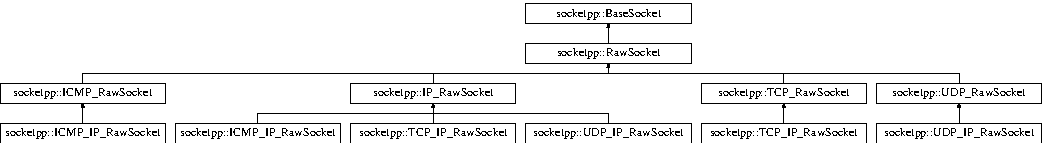
\includegraphics[height=1.9244cm]{classsocketpp_1_1RawSocket}
\end{center}
\end{figure}
\subsection*{Public Member Functions}
\begin{CompactItemize}
\item 
\hyperlink{classsocketpp_1_1RawSocket_1a77e11388869bc70457efb75cd40b82}{RawSocket} (protocol prot)
\begin{CompactList}\small\item\em constructor which calls BaseSocket(sock\_\-raw, prot) \item\end{CompactList}\item 
void \hyperlink{classsocketpp_1_1RawSocket_99ea2415525269d24ba088a58d62abdd}{build\_\-data\_\-payload} (const char $\ast$data, size\_\-t len)
\begin{CompactList}\small\item\em builds the internal data payload to send \item\end{CompactList}\item 
void \hyperlink{classsocketpp_1_1RawSocket_a5e01f4dec94dbbef1c122ce4d7ed4ad}{build\_\-data\_\-payload} (const std::string \&buf)
\begin{CompactList}\small\item\em builds the internal data payload to send \item\end{CompactList}\item 
size\_\-t \hyperlink{classsocketpp_1_1RawSocket_5c812c1bf584f40c3fc6263a8014395b}{send\_\-packet} (in\_\-addr\_\-t addr)
\begin{CompactList}\small\item\em sends the internal built packet \item\end{CompactList}\item 
size\_\-t \hyperlink{classsocketpp_1_1RawSocket_6dfb29dbfedf61d8f082dc1893320d42}{send\_\-packet} (const std::string \&addr)
\begin{CompactList}\small\item\em sends the internal built packet \item\end{CompactList}\item 
size\_\-t \hyperlink{classsocketpp_1_1RawSocket_e987bb77fd3ac6d0e99b5311ff81c1ea}{send\_\-packet} ()
\begin{CompactList}\small\item\em sends the internal built packet on a connected socket \item\end{CompactList}\item 
size\_\-t \hyperlink{classsocketpp_1_1RawSocket_1564181b6422fb3918c419051b34ae2d}{read\_\-packet} (size\_\-t len, std::string \&addr)
\begin{CompactList}\small\item\em reads the next packet on the socket \item\end{CompactList}\item 
size\_\-t \hyperlink{classsocketpp_1_1RawSocket_08b8bec945928764f2d7ee11890b8625}{read\_\-packet} (size\_\-t len, in\_\-addr\_\-t \&addr)
\begin{CompactList}\small\item\em reads the next packet on the socket \item\end{CompactList}\item 
size\_\-t \hyperlink{classsocketpp_1_1RawSocket_ea48bec4596e2afc89adba2ccb13f6c8}{read\_\-packet} (size\_\-t len)
\begin{CompactList}\small\item\em reads the next packet on the connected socket \item\end{CompactList}\item 
size\_\-t \hyperlink{classsocketpp_1_1RawSocket_bd9631abfa5165ad4ed9e2a31640d1f0}{get\_\-data\_\-payload} (char $\ast$data, size\_\-t len)
\begin{CompactList}\small\item\em gets the received data payload \item\end{CompactList}\item 
size\_\-t \hyperlink{classsocketpp_1_1RawSocket_de47c63d60cba25d1ae82f242851610d}{get\_\-data\_\-payload} (std::string \&data)
\begin{CompactList}\small\item\em gets the received data payload \item\end{CompactList}\end{CompactItemize}
\subsection*{Static Public Member Functions}
\begin{CompactItemize}
\item 
static \_\-u16 \hyperlink{classsocketpp_1_1RawSocket_bb78ecebb5bd5ab5be4ee46d786fe5cd}{checksum} (const void $\ast$buf, size\_\-t nchar)
\begin{CompactList}\small\item\em calculates internet checksum \item\end{CompactList}\item 
static \_\-u16 \hyperlink{classsocketpp_1_1RawSocket_67af2c9f3bc37146b54fc9fb69c0dd8d}{checksum} (const std::string \&buf)
\begin{CompactList}\small\item\em calculates internet checksum \item\end{CompactList}\end{CompactItemize}
\subsection*{Protected Member Functions}
\begin{CompactItemize}
\item 
\hypertarget{classsocketpp_1_1RawSocket_eb0a3f716c0fc46efa4123acf0fe1e66}{
virtual void \textbf{\_\-build\_\-packet} (std::string \&packet)=0}
\label{classsocketpp_1_1RawSocket_eb0a3f716c0fc46efa4123acf0fe1e66}

\item 
\hypertarget{classsocketpp_1_1RawSocket_45e6b041703cb8ae0f93dd19766865d5}{
virtual void \textbf{\_\-set\_\-fields} (const std::string \&packet)=0}
\label{classsocketpp_1_1RawSocket_45e6b041703cb8ae0f93dd19766865d5}

\end{CompactItemize}
\subsection*{Static Protected Member Functions}
\begin{CompactItemize}
\item 
\hypertarget{classsocketpp_1_1RawSocket_c9422942a0ed23c9900d26426a96a0ee}{
static \_\-u16 \textbf{pseudo\_\-checksum} (const void $\ast$, size\_\-t, \_\-u32, \_\-u32, \_\-u16)}
\label{classsocketpp_1_1RawSocket_c9422942a0ed23c9900d26426a96a0ee}

\end{CompactItemize}
\subsection*{Protected Attributes}
\begin{CompactItemize}
\item 
\hypertarget{classsocketpp_1_1RawSocket_4d3a1236c4ac42ab029323ae14586ff8}{
std::string \textbf{data\_\-payload}}
\label{classsocketpp_1_1RawSocket_4d3a1236c4ac42ab029323ae14586ff8}

\item 
\hypertarget{classsocketpp_1_1RawSocket_3e166c1c401c30b5721dc54f93772b36}{
std::string \textbf{rcvd\_\-data\_\-payload}}
\label{classsocketpp_1_1RawSocket_3e166c1c401c30b5721dc54f93772b36}

\end{CompactItemize}


\subsection{Detailed Description}
abstract base raw socket class. This class and all its derived classes don't require to perform any byte order conversion 

\subsection{Constructor \& Destructor Documentation}
\hypertarget{classsocketpp_1_1RawSocket_1a77e11388869bc70457efb75cd40b82}{
\index{socketpp::RawSocket@{socketpp::RawSocket}!RawSocket@{RawSocket}}
\index{RawSocket@{RawSocket}!socketpp::RawSocket@{socketpp::RawSocket}}
\subsubsection[{RawSocket}]{\setlength{\rightskip}{0pt plus 5cm}socketpp::RawSocket::RawSocket (protocol {\em prot})\hspace{0.3cm}{\tt  \mbox{[}inline\mbox{]}}}}
\label{classsocketpp_1_1RawSocket_1a77e11388869bc70457efb75cd40b82}


constructor which calls BaseSocket(sock\_\-raw, prot) 

\begin{Desc}
\item[Parameters:]
\begin{description}
\item[{\em prot}]\hyperlink{classsocketpp_1_1Socket}{Socket} protocol \end{description}
\end{Desc}


\subsection{Member Function Documentation}
\hypertarget{classsocketpp_1_1RawSocket_a5e01f4dec94dbbef1c122ce4d7ed4ad}{
\index{socketpp::RawSocket@{socketpp::RawSocket}!build\_\-data\_\-payload@{build\_\-data\_\-payload}}
\index{build\_\-data\_\-payload@{build\_\-data\_\-payload}!socketpp::RawSocket@{socketpp::RawSocket}}
\subsubsection[{build\_\-data\_\-payload}]{\setlength{\rightskip}{0pt plus 5cm}void socketpp::RawSocket::build\_\-data\_\-payload (const std::string \& {\em buf})}}
\label{classsocketpp_1_1RawSocket_a5e01f4dec94dbbef1c122ce4d7ed4ad}


builds the internal data payload to send 

\begin{Desc}
\item[Parameters:]
\begin{description}
\item[{\em buf}]data payload string \end{description}
\end{Desc}
\hypertarget{classsocketpp_1_1RawSocket_99ea2415525269d24ba088a58d62abdd}{
\index{socketpp::RawSocket@{socketpp::RawSocket}!build\_\-data\_\-payload@{build\_\-data\_\-payload}}
\index{build\_\-data\_\-payload@{build\_\-data\_\-payload}!socketpp::RawSocket@{socketpp::RawSocket}}
\subsubsection[{build\_\-data\_\-payload}]{\setlength{\rightskip}{0pt plus 5cm}void socketpp::RawSocket::build\_\-data\_\-payload (const char $\ast$ {\em data}, \/  size\_\-t {\em len})}}
\label{classsocketpp_1_1RawSocket_99ea2415525269d24ba088a58d62abdd}


builds the internal data payload to send 

\begin{Desc}
\item[Parameters:]
\begin{description}
\item[{\em data}]pointer to data payload buffer \item[{\em len}]deta length in bytes \end{description}
\end{Desc}
\hypertarget{classsocketpp_1_1RawSocket_67af2c9f3bc37146b54fc9fb69c0dd8d}{
\index{socketpp::RawSocket@{socketpp::RawSocket}!checksum@{checksum}}
\index{checksum@{checksum}!socketpp::RawSocket@{socketpp::RawSocket}}
\subsubsection[{checksum}]{\setlength{\rightskip}{0pt plus 5cm}\_\-u16 socketpp::RawSocket::checksum (const std::string \& {\em buf})\hspace{0.3cm}{\tt  \mbox{[}static\mbox{]}}}}
\label{classsocketpp_1_1RawSocket_67af2c9f3bc37146b54fc9fb69c0dd8d}


calculates internet checksum 

\begin{Desc}
\item[Parameters:]
\begin{description}
\item[{\em buf}]packet string \end{description}
\end{Desc}
\begin{Desc}
\item[Returns:]checksum value \end{Desc}
\hypertarget{classsocketpp_1_1RawSocket_bb78ecebb5bd5ab5be4ee46d786fe5cd}{
\index{socketpp::RawSocket@{socketpp::RawSocket}!checksum@{checksum}}
\index{checksum@{checksum}!socketpp::RawSocket@{socketpp::RawSocket}}
\subsubsection[{checksum}]{\setlength{\rightskip}{0pt plus 5cm}\_\-u16 socketpp::RawSocket::checksum (const void $\ast$ {\em buf}, \/  size\_\-t {\em nchar})\hspace{0.3cm}{\tt  \mbox{[}static\mbox{]}}}}
\label{classsocketpp_1_1RawSocket_bb78ecebb5bd5ab5be4ee46d786fe5cd}


calculates internet checksum 

\begin{Desc}
\item[Parameters:]
\begin{description}
\item[{\em buf}]pointer to packet top \item[{\em nchar}]size of packet in bytes \end{description}
\end{Desc}
\begin{Desc}
\item[Returns:]checksum value \end{Desc}
\hypertarget{classsocketpp_1_1RawSocket_de47c63d60cba25d1ae82f242851610d}{
\index{socketpp::RawSocket@{socketpp::RawSocket}!get\_\-data\_\-payload@{get\_\-data\_\-payload}}
\index{get\_\-data\_\-payload@{get\_\-data\_\-payload}!socketpp::RawSocket@{socketpp::RawSocket}}
\subsubsection[{get\_\-data\_\-payload}]{\setlength{\rightskip}{0pt plus 5cm}size\_\-t socketpp::RawSocket::get\_\-data\_\-payload (std::string \& {\em data})}}
\label{classsocketpp_1_1RawSocket_de47c63d60cba25d1ae82f242851610d}


gets the received data payload 

\begin{Desc}
\item[Parameters:]
\begin{description}
\item[{\em data}]string to fill with data \end{description}
\end{Desc}
\begin{Desc}
\item[Returns:]number of bytes written \end{Desc}
\hypertarget{classsocketpp_1_1RawSocket_bd9631abfa5165ad4ed9e2a31640d1f0}{
\index{socketpp::RawSocket@{socketpp::RawSocket}!get\_\-data\_\-payload@{get\_\-data\_\-payload}}
\index{get\_\-data\_\-payload@{get\_\-data\_\-payload}!socketpp::RawSocket@{socketpp::RawSocket}}
\subsubsection[{get\_\-data\_\-payload}]{\setlength{\rightskip}{0pt plus 5cm}size\_\-t socketpp::RawSocket::get\_\-data\_\-payload (char $\ast$ {\em data}, \/  size\_\-t {\em len})}}
\label{classsocketpp_1_1RawSocket_bd9631abfa5165ad4ed9e2a31640d1f0}


gets the received data payload 

\begin{Desc}
\item[Parameters:]
\begin{description}
\item[{\em data}]pointer to buffer to fill with data \item[{\em len}]max number of bytes to write on buffer \end{description}
\end{Desc}
\begin{Desc}
\item[Returns:]number of bytes written \end{Desc}
\hypertarget{classsocketpp_1_1RawSocket_ea48bec4596e2afc89adba2ccb13f6c8}{
\index{socketpp::RawSocket@{socketpp::RawSocket}!read\_\-packet@{read\_\-packet}}
\index{read\_\-packet@{read\_\-packet}!socketpp::RawSocket@{socketpp::RawSocket}}
\subsubsection[{read\_\-packet}]{\setlength{\rightskip}{0pt plus 5cm}size\_\-t socketpp::RawSocket::read\_\-packet (size\_\-t {\em len})}}
\label{classsocketpp_1_1RawSocket_ea48bec4596e2afc89adba2ccb13f6c8}


reads the next packet on the connected socket 

\begin{Desc}
\item[Parameters:]
\begin{description}
\item[{\em len}]max number of bytes to read \end{description}
\end{Desc}
\begin{Desc}
\item[Returns:]number of bytes red \end{Desc}
\hypertarget{classsocketpp_1_1RawSocket_08b8bec945928764f2d7ee11890b8625}{
\index{socketpp::RawSocket@{socketpp::RawSocket}!read\_\-packet@{read\_\-packet}}
\index{read\_\-packet@{read\_\-packet}!socketpp::RawSocket@{socketpp::RawSocket}}
\subsubsection[{read\_\-packet}]{\setlength{\rightskip}{0pt plus 5cm}size\_\-t socketpp::RawSocket::read\_\-packet (size\_\-t {\em len}, \/  in\_\-addr\_\-t \& {\em addr})}}
\label{classsocketpp_1_1RawSocket_08b8bec945928764f2d7ee11890b8625}


reads the next packet on the socket 

\begin{Desc}
\item[Parameters:]
\begin{description}
\item[{\em len}]max number of bytes to read \item[{\em addr}]in\_\-addr\_\-t to fill in with sender's address \end{description}
\end{Desc}
\begin{Desc}
\item[Returns:]number of bytes red \end{Desc}
\hypertarget{classsocketpp_1_1RawSocket_1564181b6422fb3918c419051b34ae2d}{
\index{socketpp::RawSocket@{socketpp::RawSocket}!read\_\-packet@{read\_\-packet}}
\index{read\_\-packet@{read\_\-packet}!socketpp::RawSocket@{socketpp::RawSocket}}
\subsubsection[{read\_\-packet}]{\setlength{\rightskip}{0pt plus 5cm}size\_\-t socketpp::RawSocket::read\_\-packet (size\_\-t {\em len}, \/  std::string \& {\em addr})}}
\label{classsocketpp_1_1RawSocket_1564181b6422fb3918c419051b34ae2d}


reads the next packet on the socket 

\begin{Desc}
\item[Parameters:]
\begin{description}
\item[{\em len}]max number of bytes to read \item[{\em addr}]string to fill in with sender's address \end{description}
\end{Desc}
\begin{Desc}
\item[Returns:]number of bytes red \end{Desc}
\hypertarget{classsocketpp_1_1RawSocket_e987bb77fd3ac6d0e99b5311ff81c1ea}{
\index{socketpp::RawSocket@{socketpp::RawSocket}!send\_\-packet@{send\_\-packet}}
\index{send\_\-packet@{send\_\-packet}!socketpp::RawSocket@{socketpp::RawSocket}}
\subsubsection[{send\_\-packet}]{\setlength{\rightskip}{0pt plus 5cm}size\_\-t socketpp::RawSocket::send\_\-packet ()}}
\label{classsocketpp_1_1RawSocket_e987bb77fd3ac6d0e99b5311ff81c1ea}


sends the internal built packet on a connected socket 

\begin{Desc}
\item[Returns:]number of bytes sent \end{Desc}
\hypertarget{classsocketpp_1_1RawSocket_6dfb29dbfedf61d8f082dc1893320d42}{
\index{socketpp::RawSocket@{socketpp::RawSocket}!send\_\-packet@{send\_\-packet}}
\index{send\_\-packet@{send\_\-packet}!socketpp::RawSocket@{socketpp::RawSocket}}
\subsubsection[{send\_\-packet}]{\setlength{\rightskip}{0pt plus 5cm}size\_\-t socketpp::RawSocket::send\_\-packet (const std::string \& {\em addr})}}
\label{classsocketpp_1_1RawSocket_6dfb29dbfedf61d8f082dc1893320d42}


sends the internal built packet 

\begin{Desc}
\item[Parameters:]
\begin{description}
\item[{\em addr}]destination hostname or dotted decimal address \end{description}
\end{Desc}
\begin{Desc}
\item[Returns:]number of bytes sent \end{Desc}
\hypertarget{classsocketpp_1_1RawSocket_5c812c1bf584f40c3fc6263a8014395b}{
\index{socketpp::RawSocket@{socketpp::RawSocket}!send\_\-packet@{send\_\-packet}}
\index{send\_\-packet@{send\_\-packet}!socketpp::RawSocket@{socketpp::RawSocket}}
\subsubsection[{send\_\-packet}]{\setlength{\rightskip}{0pt plus 5cm}size\_\-t socketpp::RawSocket::send\_\-packet (in\_\-addr\_\-t {\em addr})}}
\label{classsocketpp_1_1RawSocket_5c812c1bf584f40c3fc6263a8014395b}


sends the internal built packet 

\begin{Desc}
\item[Parameters:]
\begin{description}
\item[{\em addr}]destination IP address \end{description}
\end{Desc}
\begin{Desc}
\item[Returns:]number of bytes sent \end{Desc}


The documentation for this class was generated from the following files:\begin{CompactItemize}
\item 
RawSocket.h\item 
RawSocket.cpp\end{CompactItemize}

\hypertarget{classsocketpp_1_1SockBuf}{
\section{socketpp::SockBuf Class Reference}
\label{classsocketpp_1_1SockBuf}\index{socketpp::SockBuf@{socketpp::SockBuf}}
}
publicly derived from std::streambuf and \hyperlink{classsocketpp_1_1BaseSocket}{BaseSocket}  


{\tt \#include $<$SockStream.h$>$}

Inheritance diagram for socketpp::SockBuf::\begin{figure}[H]
\begin{center}
\leavevmode
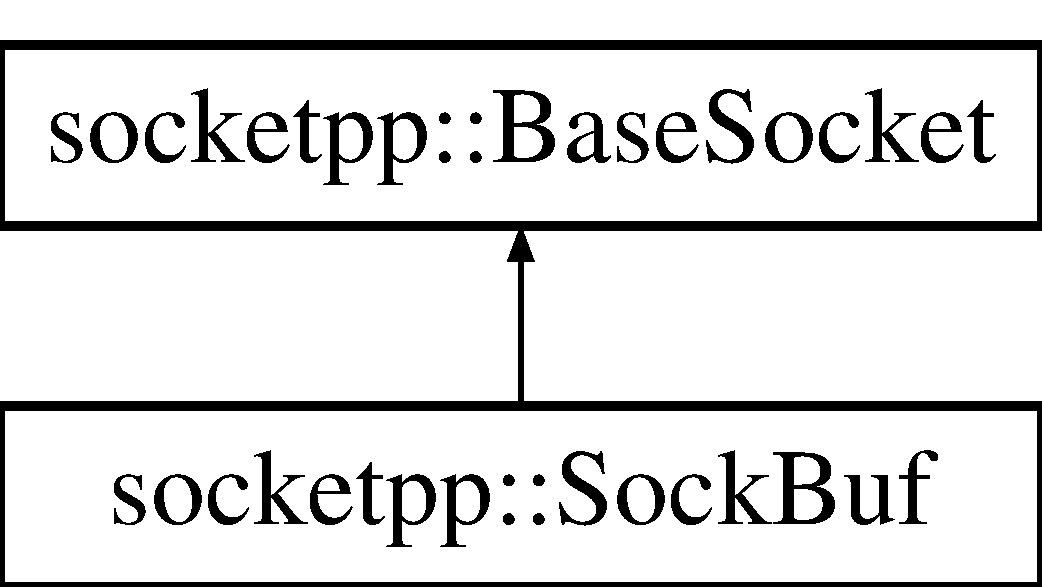
\includegraphics[height=2cm]{classsocketpp_1_1SockBuf}
\end{center}
\end{figure}
\subsection*{Public Member Functions}
\begin{CompactItemize}
\item 
\hyperlink{classsocketpp_1_1SockBuf_e02aca0e93d6b6227ba492cdc2690d9a}{SockBuf} ()
\item 
\hyperlink{classsocketpp_1_1SockBuf_065ef76cdf18c04857350c643bd620e3}{SockBuf} (const \hyperlink{classsocketpp_1_1Socket}{Socket} \&s)
\begin{CompactList}\small\item\em calls BaseSocket(s) \item\end{CompactList}\item 
\hyperlink{classsocketpp_1_1SockBuf_5e8a5860fd67228e5d39ea28f9d67341}{SockBuf} (\hyperlink{namespacesocketpp_635f4c3b3f85aba331587404d59ae52d}{type} t, \hyperlink{namespacesocketpp_2969678def1c6c8cb4102802ca82e2cf}{protocol} prot=ipproto\_\-ip)
\begin{CompactList}\small\item\em calls BaseSocket(t,prot) \item\end{CompactList}\item 
\hyperlink{classsocketpp_1_1SockBuf_71bbd8cf2bd9dd79b8067b0ef771bf23}{SockBuf} (int sd)
\begin{CompactList}\small\item\em calls BaseSocket(sd) \item\end{CompactList}\item 
void \hyperlink{classsocketpp_1_1SockBuf_28f88c6ac0570ee5e9d57e255733b0f9}{close} ()
\begin{CompactList}\small\item\em closes socket descriptor and flushes output buffer \item\end{CompactList}\item 
\hyperlink{classsocketpp_1_1SockBuf_ee857faaed622effa453c7b53749ff14}{$\sim$SockBuf} ()
\begin{CompactList}\small\item\em calls \hyperlink{classsocketpp_1_1SockBuf_28f88c6ac0570ee5e9d57e255733b0f9}{close()} \item\end{CompactList}\end{CompactItemize}
\subsection*{Static Public Attributes}
\begin{CompactItemize}
\item 
static const int \hyperlink{classsocketpp_1_1SockBuf_2b90c5705f30dd3fda03a6eb13378e15}{BUFSIZE} = BUFSIZ
\end{CompactItemize}
\subsection*{Protected Member Functions}
\begin{CompactItemize}
\item 
virtual int \hyperlink{classsocketpp_1_1SockBuf_5a1f6d2304fe83a8602e07d12032b2c7}{overflow} (int c=EOF)
\item 
virtual int \hyperlink{classsocketpp_1_1SockBuf_34ccc364e9f20a25199bea9fdde19bdd}{underflow} ()
\item 
virtual int \hyperlink{classsocketpp_1_1SockBuf_33c3d2907102b5b38daca32fb2c12591}{sync} ()
\end{CompactItemize}


\subsection{Detailed Description}
publicly derived from std::streambuf and \hyperlink{classsocketpp_1_1BaseSocket}{BaseSocket} 

\subsection{Constructor \& Destructor Documentation}
\hypertarget{classsocketpp_1_1SockBuf_e02aca0e93d6b6227ba492cdc2690d9a}{
\index{socketpp::SockBuf@{socketpp::SockBuf}!SockBuf@{SockBuf}}
\index{SockBuf@{SockBuf}!socketpp::SockBuf@{socketpp::SockBuf}}
\subsubsection[{SockBuf}]{\setlength{\rightskip}{0pt plus 5cm}socketpp::SockBuf::SockBuf ()\hspace{0.3cm}{\tt  \mbox{[}inline\mbox{]}}}}
\label{classsocketpp_1_1SockBuf_e02aca0e93d6b6227ba492cdc2690d9a}


\hypertarget{classsocketpp_1_1SockBuf_065ef76cdf18c04857350c643bd620e3}{
\index{socketpp::SockBuf@{socketpp::SockBuf}!SockBuf@{SockBuf}}
\index{SockBuf@{SockBuf}!socketpp::SockBuf@{socketpp::SockBuf}}
\subsubsection[{SockBuf}]{\setlength{\rightskip}{0pt plus 5cm}socketpp::SockBuf::SockBuf (const {\bf Socket} \& {\em s})\hspace{0.3cm}{\tt  \mbox{[}inline\mbox{]}}}}
\label{classsocketpp_1_1SockBuf_065ef76cdf18c04857350c643bd620e3}


calls BaseSocket(s) 

\hypertarget{classsocketpp_1_1SockBuf_5e8a5860fd67228e5d39ea28f9d67341}{
\index{socketpp::SockBuf@{socketpp::SockBuf}!SockBuf@{SockBuf}}
\index{SockBuf@{SockBuf}!socketpp::SockBuf@{socketpp::SockBuf}}
\subsubsection[{SockBuf}]{\setlength{\rightskip}{0pt plus 5cm}socketpp::SockBuf::SockBuf ({\bf type} {\em t}, \/  {\bf protocol} {\em prot} = {\tt ipproto\_\-ip})\hspace{0.3cm}{\tt  \mbox{[}inline\mbox{]}}}}
\label{classsocketpp_1_1SockBuf_5e8a5860fd67228e5d39ea28f9d67341}


calls BaseSocket(t,prot) 

\hypertarget{classsocketpp_1_1SockBuf_71bbd8cf2bd9dd79b8067b0ef771bf23}{
\index{socketpp::SockBuf@{socketpp::SockBuf}!SockBuf@{SockBuf}}
\index{SockBuf@{SockBuf}!socketpp::SockBuf@{socketpp::SockBuf}}
\subsubsection[{SockBuf}]{\setlength{\rightskip}{0pt plus 5cm}socketpp::SockBuf::SockBuf (int {\em sd})\hspace{0.3cm}{\tt  \mbox{[}inline\mbox{]}}}}
\label{classsocketpp_1_1SockBuf_71bbd8cf2bd9dd79b8067b0ef771bf23}


calls BaseSocket(sd) 

\hypertarget{classsocketpp_1_1SockBuf_ee857faaed622effa453c7b53749ff14}{
\index{socketpp::SockBuf@{socketpp::SockBuf}!$\sim$SockBuf@{$\sim$SockBuf}}
\index{$\sim$SockBuf@{$\sim$SockBuf}!socketpp::SockBuf@{socketpp::SockBuf}}
\subsubsection[{$\sim$SockBuf}]{\setlength{\rightskip}{0pt plus 5cm}socketpp::SockBuf::$\sim$SockBuf ()}}
\label{classsocketpp_1_1SockBuf_ee857faaed622effa453c7b53749ff14}


calls \hyperlink{classsocketpp_1_1SockBuf_28f88c6ac0570ee5e9d57e255733b0f9}{close()} 



\subsection{Member Function Documentation}
\hypertarget{classsocketpp_1_1SockBuf_28f88c6ac0570ee5e9d57e255733b0f9}{
\index{socketpp::SockBuf@{socketpp::SockBuf}!close@{close}}
\index{close@{close}!socketpp::SockBuf@{socketpp::SockBuf}}
\subsubsection[{close}]{\setlength{\rightskip}{0pt plus 5cm}void socketpp::SockBuf::close ()\hspace{0.3cm}{\tt  \mbox{[}virtual\mbox{]}}}}
\label{classsocketpp_1_1SockBuf_28f88c6ac0570ee5e9d57e255733b0f9}


closes socket descriptor and flushes output buffer 



Reimplemented from \hyperlink{classsocketpp_1_1BaseSocket_f067195056bb6b5a65c4bc1d2ac7da72}{socketpp::BaseSocket}.\hypertarget{classsocketpp_1_1SockBuf_5a1f6d2304fe83a8602e07d12032b2c7}{
\index{socketpp::SockBuf@{socketpp::SockBuf}!overflow@{overflow}}
\index{overflow@{overflow}!socketpp::SockBuf@{socketpp::SockBuf}}
\subsubsection[{overflow}]{\setlength{\rightskip}{0pt plus 5cm}int socketpp::SockBuf::overflow (int {\em c} = {\tt EOF})\hspace{0.3cm}{\tt  \mbox{[}protected, virtual\mbox{]}}}}
\label{classsocketpp_1_1SockBuf_5a1f6d2304fe83a8602e07d12032b2c7}


\hypertarget{classsocketpp_1_1SockBuf_33c3d2907102b5b38daca32fb2c12591}{
\index{socketpp::SockBuf@{socketpp::SockBuf}!sync@{sync}}
\index{sync@{sync}!socketpp::SockBuf@{socketpp::SockBuf}}
\subsubsection[{sync}]{\setlength{\rightskip}{0pt plus 5cm}int socketpp::SockBuf::sync ()\hspace{0.3cm}{\tt  \mbox{[}protected, virtual\mbox{]}}}}
\label{classsocketpp_1_1SockBuf_33c3d2907102b5b38daca32fb2c12591}


\hypertarget{classsocketpp_1_1SockBuf_34ccc364e9f20a25199bea9fdde19bdd}{
\index{socketpp::SockBuf@{socketpp::SockBuf}!underflow@{underflow}}
\index{underflow@{underflow}!socketpp::SockBuf@{socketpp::SockBuf}}
\subsubsection[{underflow}]{\setlength{\rightskip}{0pt plus 5cm}int socketpp::SockBuf::underflow ()\hspace{0.3cm}{\tt  \mbox{[}protected, virtual\mbox{]}}}}
\label{classsocketpp_1_1SockBuf_34ccc364e9f20a25199bea9fdde19bdd}




\subsection{Member Data Documentation}
\hypertarget{classsocketpp_1_1SockBuf_2b90c5705f30dd3fda03a6eb13378e15}{
\index{socketpp::SockBuf@{socketpp::SockBuf}!BUFSIZE@{BUFSIZE}}
\index{BUFSIZE@{BUFSIZE}!socketpp::SockBuf@{socketpp::SockBuf}}
\subsubsection[{BUFSIZE}]{\setlength{\rightskip}{0pt plus 5cm}const int {\bf socketpp::SockBuf::BUFSIZE} = BUFSIZ\hspace{0.3cm}{\tt  \mbox{[}static\mbox{]}}}}
\label{classsocketpp_1_1SockBuf_2b90c5705f30dd3fda03a6eb13378e15}




The documentation for this class was generated from the following files:\begin{CompactItemize}
\item 
\hyperlink{SockStream_8h}{SockStream.h}\item 
\hyperlink{SockStream_8cpp}{SockStream.cpp}\end{CompactItemize}

\hypertarget{classsocketpp_1_1Socket}{
\section{socketpp::Socket Class Reference}
\label{classsocketpp_1_1Socket}\index{socketpp::Socket@{socketpp::Socket}}
}
inherits from \hyperlink{classsocketpp_1_1BaseSocket}{BaseSocket}, it's simply a C-socket wrapper  


{\tt \#include $<$Socket.h$>$}

Inheritance diagram for socketpp::Socket::\begin{figure}[H]
\begin{center}
\leavevmode
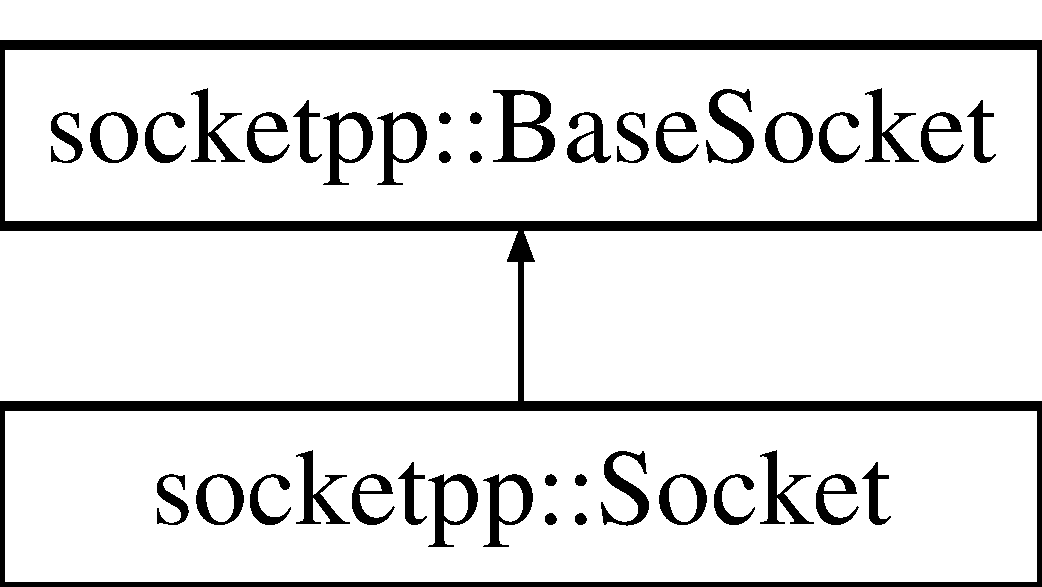
\includegraphics[height=2cm]{classsocketpp_1_1Socket}
\end{center}
\end{figure}
\subsection*{Public Member Functions}
\begin{CompactItemize}
\item 
\hypertarget{classsocketpp_1_1Socket_c10e4f533ed78a3d898c1fe0cea09cef}{
\hyperlink{classsocketpp_1_1Socket_c10e4f533ed78a3d898c1fe0cea09cef}{Socket} (type t, protocol prot=ipproto\_\-ip)}
\label{classsocketpp_1_1Socket_c10e4f533ed78a3d898c1fe0cea09cef}

\begin{CompactList}\small\item\em calls BaseSocket(t,prot) \item\end{CompactList}\item 
\hypertarget{classsocketpp_1_1Socket_2ec875f75becab573f7720d50ab13c99}{
\hyperlink{classsocketpp_1_1Socket_2ec875f75becab573f7720d50ab13c99}{Socket} (int sd)}
\label{classsocketpp_1_1Socket_2ec875f75becab573f7720d50ab13c99}

\begin{CompactList}\small\item\em calls BaseSocket(sd) \item\end{CompactList}\end{CompactItemize}


\subsection{Detailed Description}
inherits from \hyperlink{classsocketpp_1_1BaseSocket}{BaseSocket}, it's simply a C-socket wrapper 

The documentation for this class was generated from the following file:\begin{CompactItemize}
\item 
Socket.h\end{CompactItemize}

\hypertarget{classsocketpp_1_1SocketServer}{
\section{socketpp::SocketServer Class Reference}
\label{classsocketpp_1_1SocketServer}\index{socketpp::SocketServer@{socketpp::SocketServer}}
}
TCP server class which can accept simultaneously multiple connections through multithreading.  


{\tt \#include $<$SocketServer.h$>$}

Inheritance diagram for socketpp::SocketServer::\begin{figure}[H]
\begin{center}
\leavevmode
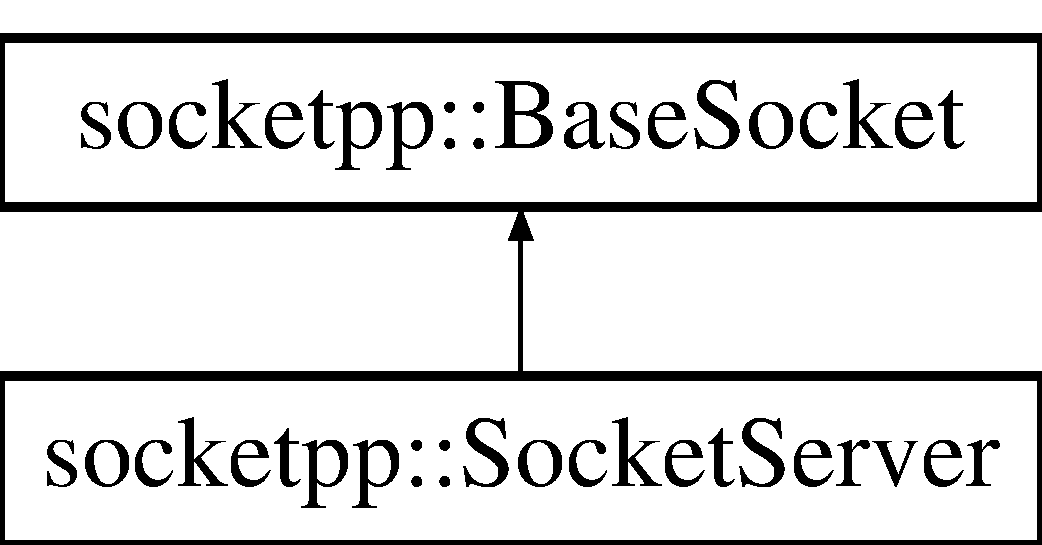
\includegraphics[height=2cm]{classsocketpp_1_1SocketServer}
\end{center}
\end{figure}
\subsection*{Public Member Functions}
\begin{CompactItemize}
\item 
\hypertarget{classsocketpp_1_1SocketServer_3a6955b6d5617457cf31206ea9492786}{
\hyperlink{classsocketpp_1_1SocketServer_3a6955b6d5617457cf31206ea9492786}{SocketServer} (type t)}
\label{classsocketpp_1_1SocketServer_3a6955b6d5617457cf31206ea9492786}

\begin{CompactList}\small\item\em calls BaseSocket(t) \item\end{CompactList}\item 
\hypertarget{classsocketpp_1_1SocketServer_e83ff222d6d4dd600dc162926afdac0f}{
\hyperlink{classsocketpp_1_1SocketServer_e83ff222d6d4dd600dc162926afdac0f}{SocketServer} (const \hyperlink{classsocketpp_1_1SocketServer}{SocketServer} \&s)}
\label{classsocketpp_1_1SocketServer_e83ff222d6d4dd600dc162926afdac0f}

\begin{CompactList}\small\item\em copy constructor \item\end{CompactList}\item 
\hyperlink{classsocketpp_1_1SocketServer_73c5125f9e5a6cf03dc15f6d4250e345}{SocketServer} (type t, in\_\-addr\_\-t addr, port\_\-t port, unsigned int maxconn=0)
\begin{CompactList}\small\item\em binds socket and puts it in listening mode \item\end{CompactList}\item 
\hyperlink{classsocketpp_1_1SocketServer_2b43397fd614dc7953559d7372f1c6ca}{SocketServer} (type t, const std::string \&addr, port\_\-t port, unsigned int maxconn=0)
\begin{CompactList}\small\item\em binds socket and puts it in listening mode \item\end{CompactList}\item 
\hyperlink{classsocketpp_1_1SocketServer_594f3a739f4cd053f9fd0512e42473be}{SocketServer} (type t, in\_\-addr\_\-t addr, const std::string \&serv, const char $\ast$prot=NULL, unsigned int maxconn=0)
\begin{CompactList}\small\item\em binds socket and puts it in listening mode \item\end{CompactList}\item 
\hyperlink{classsocketpp_1_1SocketServer_667f8c2b7b1325c80f018ecf85a9551f}{SocketServer} (type t, const std::string \&addr, const std::string \&serv, const char $\ast$prot=NULL, unsigned int maxconn=0)
\begin{CompactList}\small\item\em binds socket and puts it in listening mode \item\end{CompactList}\item 
\hyperlink{classsocketpp_1_1Socket}{Socket} \& \hyperlink{classsocketpp_1_1SocketServer_de24bd723d353d62d034718a1d95c02f}{accept} ()
\begin{CompactList}\small\item\em Accepts connection request. \item\end{CompactList}\item 
int \hyperlink{classsocketpp_1_1SocketServer_034ddc2def5342b5a26264ffcb9e8e36}{listen} (int maxconn)
\begin{CompactList}\small\item\em puts socket in listening mode \item\end{CompactList}\item 
void \hyperlink{classsocketpp_1_1SocketServer_0ded92a6348a6cf953d9f646fac43ac2}{threadClientHandle} (void($\ast$f)(\hyperlink{classsocketpp_1_1Socket}{Socket} \&, void $\ast$), void $\ast$pt)
\begin{CompactList}\small\item\em puts server in multithreaded mode \item\end{CompactList}\end{CompactItemize}


\subsection{Detailed Description}
TCP server class which can accept simultaneously multiple connections through multithreading. 

\subsection{Constructor \& Destructor Documentation}
\hypertarget{classsocketpp_1_1SocketServer_73c5125f9e5a6cf03dc15f6d4250e345}{
\index{socketpp::SocketServer@{socketpp::SocketServer}!SocketServer@{SocketServer}}
\index{SocketServer@{SocketServer}!socketpp::SocketServer@{socketpp::SocketServer}}
\subsubsection{\setlength{\rightskip}{0pt plus 5cm}socketpp::SocketServer::SocketServer (type {\em t}, \/  in\_\-addr\_\-t {\em addr}, \/  port\_\-t {\em port}, \/  unsigned int {\em maxconn} = {\tt 0})}}
\label{classsocketpp_1_1SocketServer_73c5125f9e5a6cf03dc15f6d4250e345}


binds socket and puts it in listening mode 

\begin{Desc}
\item[Parameters:]
\begin{description}
\item[{\em t}]socket type \item[{\em addr}]numerical local address to bind \item[{\em port}]local port to bind \item[{\em maxconn}]max number of connections to accept \end{description}
\end{Desc}
\hypertarget{classsocketpp_1_1SocketServer_2b43397fd614dc7953559d7372f1c6ca}{
\index{socketpp::SocketServer@{socketpp::SocketServer}!SocketServer@{SocketServer}}
\index{SocketServer@{SocketServer}!socketpp::SocketServer@{socketpp::SocketServer}}
\subsubsection{\setlength{\rightskip}{0pt plus 5cm}socketpp::SocketServer::SocketServer (type {\em t}, \/  const std::string \& {\em addr}, \/  port\_\-t {\em port}, \/  unsigned int {\em maxconn} = {\tt 0})}}
\label{classsocketpp_1_1SocketServer_2b43397fd614dc7953559d7372f1c6ca}


binds socket and puts it in listening mode 

\begin{Desc}
\item[Parameters:]
\begin{description}
\item[{\em t}]socket type \item[{\em addr}]dotted decimal local address to bind \item[{\em port}]local port to bind \item[{\em maxconn}]max number of connections to accept \end{description}
\end{Desc}
\hypertarget{classsocketpp_1_1SocketServer_594f3a739f4cd053f9fd0512e42473be}{
\index{socketpp::SocketServer@{socketpp::SocketServer}!SocketServer@{SocketServer}}
\index{SocketServer@{SocketServer}!socketpp::SocketServer@{socketpp::SocketServer}}
\subsubsection{\setlength{\rightskip}{0pt plus 5cm}socketpp::SocketServer::SocketServer (type {\em t}, \/  in\_\-addr\_\-t {\em addr}, \/  const std::string \& {\em serv}, \/  const char $\ast$ {\em prot} = {\tt NULL}, \/  unsigned int {\em maxconn} = {\tt 0})}}
\label{classsocketpp_1_1SocketServer_594f3a739f4cd053f9fd0512e42473be}


binds socket and puts it in listening mode 

\begin{Desc}
\item[Parameters:]
\begin{description}
\item[{\em t}]socket type \item[{\em addr}]numerical local address to bind \item[{\em serv}]local service to bind \item[{\em prot}]transport layer protocol \item[{\em maxconn}]max number of connections to accept \end{description}
\end{Desc}
\hypertarget{classsocketpp_1_1SocketServer_667f8c2b7b1325c80f018ecf85a9551f}{
\index{socketpp::SocketServer@{socketpp::SocketServer}!SocketServer@{SocketServer}}
\index{SocketServer@{SocketServer}!socketpp::SocketServer@{socketpp::SocketServer}}
\subsubsection{\setlength{\rightskip}{0pt plus 5cm}socketpp::SocketServer::SocketServer (type {\em t}, \/  const std::string \& {\em addr}, \/  const std::string \& {\em serv}, \/  const char $\ast$ {\em prot} = {\tt NULL}, \/  unsigned int {\em maxconn} = {\tt 0})}}
\label{classsocketpp_1_1SocketServer_667f8c2b7b1325c80f018ecf85a9551f}


binds socket and puts it in listening mode 

\begin{Desc}
\item[Parameters:]
\begin{description}
\item[{\em t}]socket type \item[{\em addr}]dotted decimal local address to bind \item[{\em serv}]local service to bind \item[{\em prot}]transport layer protocol \item[{\em maxconn}]max number of connections to accept \end{description}
\end{Desc}


\subsection{Member Function Documentation}
\hypertarget{classsocketpp_1_1SocketServer_de24bd723d353d62d034718a1d95c02f}{
\index{socketpp::SocketServer@{socketpp::SocketServer}!accept@{accept}}
\index{accept@{accept}!socketpp::SocketServer@{socketpp::SocketServer}}
\subsubsection{\setlength{\rightskip}{0pt plus 5cm}{\bf Socket} \& socketpp::SocketServer::accept ()}}
\label{classsocketpp_1_1SocketServer_de24bd723d353d62d034718a1d95c02f}


Accepts connection request. 

\begin{Desc}
\item[Returns:]connected socket object \end{Desc}
\hypertarget{classsocketpp_1_1SocketServer_034ddc2def5342b5a26264ffcb9e8e36}{
\index{socketpp::SocketServer@{socketpp::SocketServer}!listen@{listen}}
\index{listen@{listen}!socketpp::SocketServer@{socketpp::SocketServer}}
\subsubsection{\setlength{\rightskip}{0pt plus 5cm}int socketpp::SocketServer::listen (int {\em maxconn})}}
\label{classsocketpp_1_1SocketServer_034ddc2def5342b5a26264ffcb9e8e36}


puts socket in listening mode 

\begin{Desc}
\item[Parameters:]
\begin{description}
\item[{\em maxconn}]max number of connections to accept \end{description}
\end{Desc}
\hypertarget{classsocketpp_1_1SocketServer_0ded92a6348a6cf953d9f646fac43ac2}{
\index{socketpp::SocketServer@{socketpp::SocketServer}!threadClientHandle@{threadClientHandle}}
\index{threadClientHandle@{threadClientHandle}!socketpp::SocketServer@{socketpp::SocketServer}}
\subsubsection{\setlength{\rightskip}{0pt plus 5cm}void socketpp::SocketServer::threadClientHandle (void($\ast$)({\bf Socket} \&, void $\ast$) {\em f}, \/  void $\ast$ {\em pt})}}
\label{classsocketpp_1_1SocketServer_0ded92a6348a6cf953d9f646fac43ac2}


puts server in multithreaded mode 

\begin{Desc}
\item[Parameters:]
\begin{description}
\item[{\em f}]function to call when a connection is accepted, it requires as arguments the connected socket and a void pointer \item[{\em pt}]pointer to arguments accepted by function f \end{description}
\end{Desc}


The documentation for this class was generated from the following files:\begin{CompactItemize}
\item 
SocketServer.h\item 
SocketServer.cpp\end{CompactItemize}

\hypertarget{classsocketpp_1_1SockStream}{
\section{socketpp::SockStream Class Reference}
\label{classsocketpp_1_1SockStream}\index{socketpp::SockStream@{socketpp::SockStream}}
}
inherits from std::iostream, it allows the C++ stream approach with sockets  


{\tt \#include $<$SockStream.h$>$}

\subsection*{Public Member Functions}
\begin{CompactItemize}
\item 
\hypertarget{classsocketpp_1_1SockStream_11fbfc7bda45c178c6e09ac6d67512fd}{
\hyperlink{classsocketpp_1_1SockStream_11fbfc7bda45c178c6e09ac6d67512fd}{SockStream} (\hyperlink{classsocketpp_1_1SockBuf}{SockBuf} \&s)}
\label{classsocketpp_1_1SockStream_11fbfc7bda45c178c6e09ac6d67512fd}

\begin{CompactList}\small\item\em calls std::iostream(\&s) \item\end{CompactList}\item 
\hypertarget{classsocketpp_1_1SockStream_704f4e77af424bd0638e736653e2d1b3}{
\hyperlink{classsocketpp_1_1SockStream_704f4e77af424bd0638e736653e2d1b3}{SockStream} (const \hyperlink{classsocketpp_1_1Socket}{Socket} \&s)}
\label{classsocketpp_1_1SockStream_704f4e77af424bd0638e736653e2d1b3}

\begin{CompactList}\small\item\em calls std::iostream(new SockBuf(s)) \item\end{CompactList}\item 
\hypertarget{classsocketpp_1_1SockStream_0310cdd1f212beec6b686d0a549f1788}{
\hyperlink{classsocketpp_1_1SockStream_0310cdd1f212beec6b686d0a549f1788}{SockStream} (const \hyperlink{classsocketpp_1_1SockStream}{SockStream} \&s)}
\label{classsocketpp_1_1SockStream_0310cdd1f212beec6b686d0a549f1788}

\begin{CompactList}\small\item\em copy constructor \item\end{CompactList}\item 
\hypertarget{classsocketpp_1_1SockStream_4baa8d20dd73480832c7dd9cbad15f75}{
\hyperlink{classsocketpp_1_1SockStream_4baa8d20dd73480832c7dd9cbad15f75}{SockStream} (type t, protocol prot=ipproto\_\-ip)}
\label{classsocketpp_1_1SockStream_4baa8d20dd73480832c7dd9cbad15f75}

\begin{CompactList}\small\item\em calls std::iostream(new SockBuf(t,prot)) \item\end{CompactList}\item 
\hypertarget{classsocketpp_1_1SockStream_4b14a0ce8d640deb5f5bd64807c7b68d}{
\hyperlink{classsocketpp_1_1SockBuf}{SockBuf} $\ast$ \hyperlink{classsocketpp_1_1SockStream_4b14a0ce8d640deb5f5bd64807c7b68d}{sockbuf} () const }
\label{classsocketpp_1_1SockStream_4b14a0ce8d640deb5f5bd64807c7b68d}

\begin{CompactList}\small\item\em returns pointer to internal \hyperlink{classsocketpp_1_1SockBuf}{SockBuf} object \item\end{CompactList}\item 
\hypertarget{classsocketpp_1_1SockStream_c5509fd039943c07c4506e42c75605e3}{
\hyperlink{classsocketpp_1_1SockBuf}{SockBuf} $\ast$ \hyperlink{classsocketpp_1_1SockStream_c5509fd039943c07c4506e42c75605e3}{operator $\rightarrow$ } ()}
\label{classsocketpp_1_1SockStream_c5509fd039943c07c4506e42c75605e3}

\begin{CompactList}\small\item\em operates on internal \hyperlink{classsocketpp_1_1SockBuf}{SockBuf} object \item\end{CompactList}\end{CompactItemize}


\subsection{Detailed Description}
inherits from std::iostream, it allows the C++ stream approach with sockets 

The documentation for this class was generated from the following file:\begin{CompactItemize}
\item 
SockStream.h\end{CompactItemize}

\hypertarget{classsocketpp_1_1TCP__IP__RawSocket}{
\section{socketpp::TCP\_\-IP\_\-RawSocket Class Reference}
\label{classsocketpp_1_1TCP__IP__RawSocket}\index{socketpp::TCP\_\-IP\_\-RawSocket@{socketpp::TCP\_\-IP\_\-RawSocket}}
}
TCP raw socket with IP header handling.  


{\tt \#include $<$RawSocket.h$>$}

Inheritance diagram for socketpp::TCP\_\-IP\_\-RawSocket::\begin{figure}[H]
\begin{center}
\leavevmode
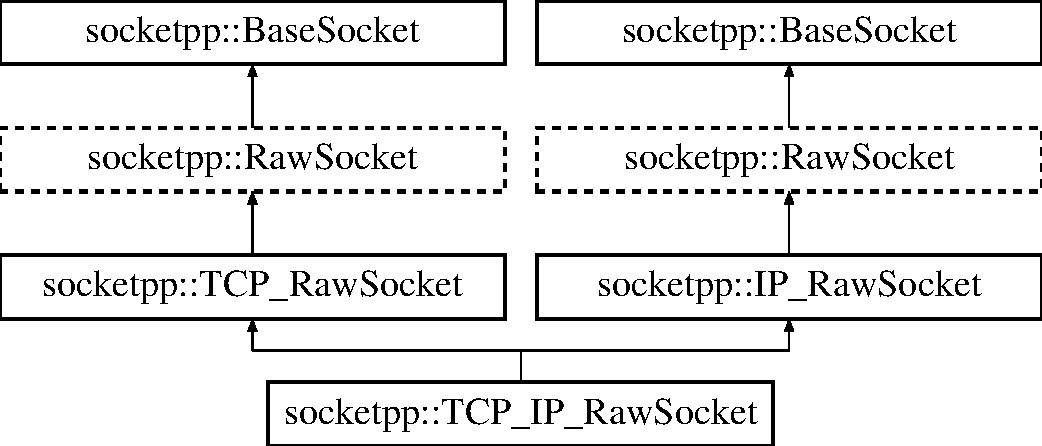
\includegraphics[height=4cm]{classsocketpp_1_1TCP__IP__RawSocket}
\end{center}
\end{figure}
\subsection*{Public Member Functions}
\begin{CompactItemize}
\item 
\hypertarget{classsocketpp_1_1TCP__IP__RawSocket_10edb8c09e89f09c0b99b5b2febce821}{
void \hyperlink{classsocketpp_1_1TCP__IP__RawSocket_10edb8c09e89f09c0b99b5b2febce821}{build\_\-IP\_\-header} (\_\-u32 saddr, \_\-u32 daddr, \_\-u8 ttl=64, \_\-u8 version=4, \_\-u8 protocol=IPPROTO\_\-TCP, \_\-u16 id=0, \_\-u8 tos=0, \_\-u16 frag\_\-off=0, \_\-u8 ihl=0, \_\-u16 tot\_\-len=0, \_\-u16 check=0)}
\label{classsocketpp_1_1TCP__IP__RawSocket_10edb8c09e89f09c0b99b5b2febce821}

\begin{CompactList}\small\item\em builds the internal IP header to send \item\end{CompactList}\item 
\hypertarget{classsocketpp_1_1TCP__IP__RawSocket_1b08f12274fd9590f805bc876c44edd9}{
\hyperlink{classsocketpp_1_1TCP__IP__RawSocket_1b08f12274fd9590f805bc876c44edd9}{TCP\_\-IP\_\-RawSocket} ()}
\label{classsocketpp_1_1TCP__IP__RawSocket_1b08f12274fd9590f805bc876c44edd9}

\begin{CompactList}\small\item\em constructor which calls RawSocket(ipproto\_\-tcp) and setsockopt(ip\_\-hdrincl) \item\end{CompactList}\item 
\hypertarget{classsocketpp_1_1TCP__IP__RawSocket_cabdd9a217d59c0c2c5511e01c222427}{
void \hyperlink{classsocketpp_1_1TCP__IP__RawSocket_cabdd9a217d59c0c2c5511e01c222427}{adjust\_\-IP\_\-csum} ()}
\label{classsocketpp_1_1TCP__IP__RawSocket_cabdd9a217d59c0c2c5511e01c222427}

\begin{CompactList}\small\item\em sets IP checksum field \item\end{CompactList}\item 
\hypertarget{classsocketpp_1_1TCP__IP__RawSocket_e9c3cfe3d011cbf85653240aa30f3f17}{
void \hyperlink{classsocketpp_1_1TCP__IP__RawSocket_e9c3cfe3d011cbf85653240aa30f3f17}{adjust\_\-IP\_\-tot\_\-len} ()}
\label{classsocketpp_1_1TCP__IP__RawSocket_e9c3cfe3d011cbf85653240aa30f3f17}

\begin{CompactList}\small\item\em sets IP \char`\"{}total length\char`\"{} field \item\end{CompactList}\item 
\hypertarget{classsocketpp_1_1TCP__IP__RawSocket_c203b188308532333bdf53a4e18bc230}{
void \hyperlink{classsocketpp_1_1TCP__IP__RawSocket_c203b188308532333bdf53a4e18bc230}{adjust\_\-TCP\_\-csum} ()}
\label{classsocketpp_1_1TCP__IP__RawSocket_c203b188308532333bdf53a4e18bc230}

\begin{CompactList}\small\item\em sets TCP checksum, using source and dest IP addresses token by IP header \item\end{CompactList}\item 
\hypertarget{classsocketpp_1_1TCP__IP__RawSocket_3644327ff72d322ff809ac432f59783b}{
void \hyperlink{classsocketpp_1_1TCP__IP__RawSocket_3644327ff72d322ff809ac432f59783b}{adjust\_\-TCP\_\-all} ()}
\label{classsocketpp_1_1TCP__IP__RawSocket_3644327ff72d322ff809ac432f59783b}

\begin{CompactList}\small\item\em calls \hyperlink{classsocketpp_1_1TCP__RawSocket_029eb8bfbf19531253edf046775d9f5f}{adjust\_\-TCP\_\-doff()} \&\& \hyperlink{classsocketpp_1_1TCP__IP__RawSocket_c203b188308532333bdf53a4e18bc230}{adjust\_\-TCP\_\-csum()} \item\end{CompactList}\item 
\hypertarget{classsocketpp_1_1TCP__IP__RawSocket_dd3b21314f1768962bf399291f406768}{
void \hyperlink{classsocketpp_1_1TCP__IP__RawSocket_dd3b21314f1768962bf399291f406768}{adjust\_\-TCP\_\-IP\_\-all} ()}
\label{classsocketpp_1_1TCP__IP__RawSocket_dd3b21314f1768962bf399291f406768}

\begin{CompactList}\small\item\em calls \hyperlink{classsocketpp_1_1TCP__IP__RawSocket_3644327ff72d322ff809ac432f59783b}{adjust\_\-TCP\_\-all()} \&\& \hyperlink{classsocketpp_1_1IP__RawSocket_45e60510233daaa2f279d3a4706fdce5}{adjust\_\-IP\_\-all()} \item\end{CompactList}\end{CompactItemize}
\subsection*{Static Public Member Functions}
\begin{CompactItemize}
\item 
\hypertarget{classsocketpp_1_1TCP__IP__RawSocket_abc1c7904d5086de03ab11ae151813a7}{
static \_\-u16 \textbf{ip\_\-checksum} (const struct iphdr \&ip, const struct tcphdr \&tcp, const void $\ast$payload=NULL, size\_\-t psize=0, const void $\ast$ip\_\-opt=NULL, size\_\-t ip\_\-opt\_\-len=0, const void $\ast$tcp\_\-opt=NULL, size\_\-t tcp\_\-opt\_\-len=0)}
\label{classsocketpp_1_1TCP__IP__RawSocket_abc1c7904d5086de03ab11ae151813a7}

\item 
\hypertarget{classsocketpp_1_1TCP__IP__RawSocket_1fcccb3c1d1454997c08e7afe1518df7}{
static \_\-u16 \textbf{ip\_\-checksum} (const struct iphdr \&ip, const struct tcphdr \&tcp, const std::string \&payload, const std::string \&ip\_\-opt, const std::string \&tcp\_\-opt)}
\label{classsocketpp_1_1TCP__IP__RawSocket_1fcccb3c1d1454997c08e7afe1518df7}

\end{CompactItemize}
\subsection*{Protected Member Functions}
\begin{CompactItemize}
\item 
\hypertarget{classsocketpp_1_1TCP__IP__RawSocket_e624076d0f5f1f63bd8c13e97a7e46ce}{
void \textbf{\_\-build\_\-packet} (std::string \&packet) const }
\label{classsocketpp_1_1TCP__IP__RawSocket_e624076d0f5f1f63bd8c13e97a7e46ce}

\item 
\hypertarget{classsocketpp_1_1TCP__IP__RawSocket_f8f606ce33835813cc5c3a530e181432}{
void \textbf{\_\-set\_\-fields} (const std::string \&packet)}
\label{classsocketpp_1_1TCP__IP__RawSocket_f8f606ce33835813cc5c3a530e181432}

\end{CompactItemize}


\subsection{Detailed Description}
TCP raw socket with IP header handling. 

The documentation for this class was generated from the following files:\begin{CompactItemize}
\item 
RawSocket.h\item 
RawSocket.cpp\end{CompactItemize}

\hypertarget{classsocketpp_1_1TCP__RawSocket}{
\section{socketpp::TCP\_\-RawSocket Class Reference}
\label{classsocketpp_1_1TCP__RawSocket}\index{socketpp::TCP\_\-RawSocket@{socketpp::TCP\_\-RawSocket}}
}
TCP raw socket without IP header handling.  


{\tt \#include $<$RawSocket.h$>$}

Inheritance diagram for socketpp::TCP\_\-RawSocket::\begin{figure}[H]
\begin{center}
\leavevmode
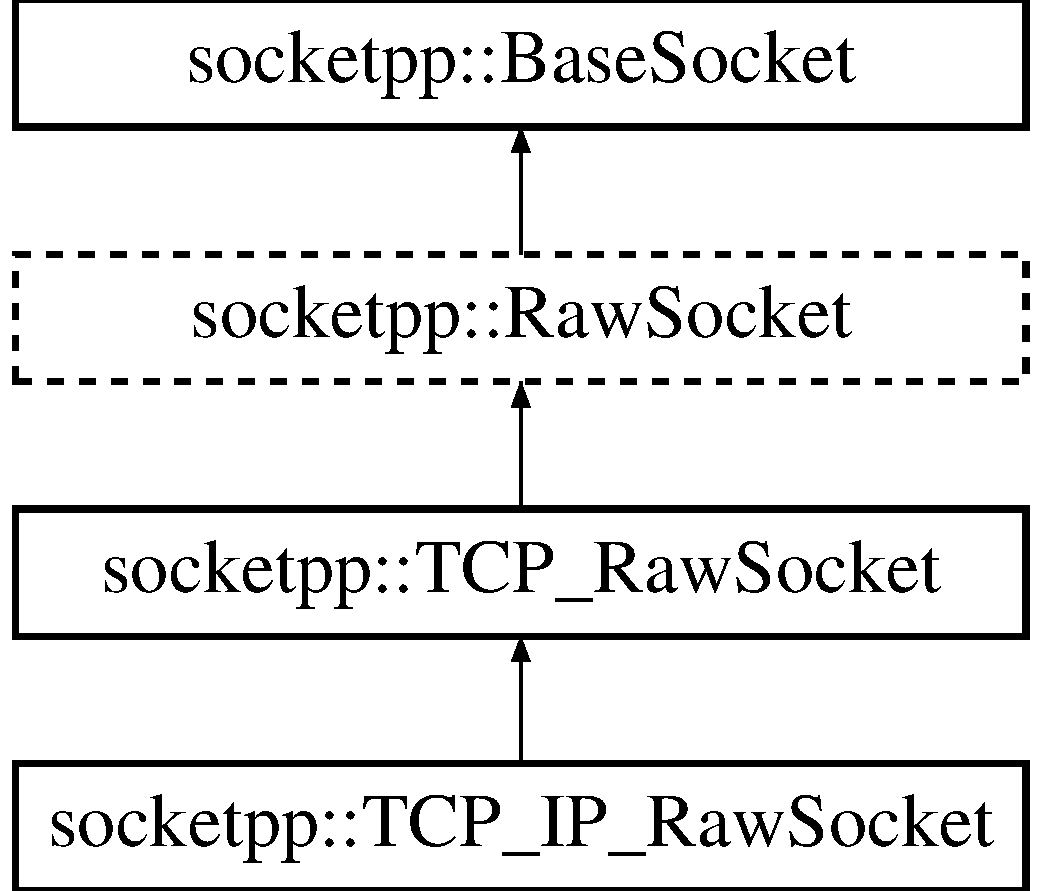
\includegraphics[height=4cm]{classsocketpp_1_1TCP__RawSocket}
\end{center}
\end{figure}
\subsection*{Public Member Functions}
\begin{CompactItemize}
\item 
\hypertarget{classsocketpp_1_1TCP__RawSocket_f0b76c8fdc293bb5e22914b247b1e7b8}{
\hyperlink{classsocketpp_1_1TCP__RawSocket_f0b76c8fdc293bb5e22914b247b1e7b8}{TCP\_\-RawSocket} ()}
\label{classsocketpp_1_1TCP__RawSocket_f0b76c8fdc293bb5e22914b247b1e7b8}

\begin{CompactList}\small\item\em constructor which calls RawSocket(ipproto\_\-tcp) \item\end{CompactList}\item 
\hypertarget{classsocketpp_1_1TCP__RawSocket_443f8b89224427ae95d22b9b305a4990}{
void \hyperlink{classsocketpp_1_1TCP__RawSocket_443f8b89224427ae95d22b9b305a4990}{build\_\-TCP\_\-header} (\_\-u16 source, \_\-u16 dest, \_\-u32 seq, \_\-u32 ack\_\-seq, \_\-u8 res1, \_\-u8 doff, \_\-u8 fin, \_\-u8 syn, \_\-u8 rst, \_\-u8 psh, \_\-u8 ack, \_\-u8 urg, \_\-u8 ece, \_\-u8 cwr, \_\-u16 window, \_\-u16 check, \_\-u16 urg\_\-ptr)}
\label{classsocketpp_1_1TCP__RawSocket_443f8b89224427ae95d22b9b305a4990}

\begin{CompactList}\small\item\em builds the internal TCP header \item\end{CompactList}\item 
void \hyperlink{classsocketpp_1_1TCP__RawSocket_8c35edfc4d8c2fbccf0fe13485dd2ef1}{build\_\-TCP\_\-header} (const tcphdr \&tcp)
\begin{CompactList}\small\item\em builds the internal TCP header \item\end{CompactList}\item 
void \hyperlink{classsocketpp_1_1TCP__RawSocket_c38e057fc6ece02026e71b7ee872533f}{set\_\-TCP\_\-options} (const char $\ast$opt, size\_\-t len)
\begin{CompactList}\small\item\em sets the TCP options field \item\end{CompactList}\item 
void \hyperlink{classsocketpp_1_1TCP__RawSocket_7bc9043e86c6f328cb99d98c4bfca05a}{set\_\-TCP\_\-options} (const std::string \&opt)
\begin{CompactList}\small\item\em sets the TCP options field \item\end{CompactList}\item 
void \hyperlink{classsocketpp_1_1TCP__RawSocket_c1a2ef8b2661bb0f3ca3fa6a636b25fd}{adjust\_\-TCP\_\-csum} (in\_\-addr\_\-t source, in\_\-addr\_\-t dest)
\begin{CompactList}\small\item\em sets the internal TCP pseudo-header checksum \item\end{CompactList}\item 
\hypertarget{classsocketpp_1_1TCP__RawSocket_029eb8bfbf19531253edf046775d9f5f}{
void \hyperlink{classsocketpp_1_1TCP__RawSocket_029eb8bfbf19531253edf046775d9f5f}{adjust\_\-TCP\_\-doff} ()}
\label{classsocketpp_1_1TCP__RawSocket_029eb8bfbf19531253edf046775d9f5f}

\begin{CompactList}\small\item\em sets the internal header \char`\"{}doff\char`\"{} field \item\end{CompactList}\item 
void \hyperlink{classsocketpp_1_1TCP__RawSocket_0a1017145ae76253dfca51cbd672fae7}{adjust\_\-TCP\_\-all} (in\_\-addr\_\-t source, in\_\-addr\_\-t dest)
\begin{CompactList}\small\item\em calls \hyperlink{classsocketpp_1_1TCP__RawSocket_029eb8bfbf19531253edf046775d9f5f}{adjust\_\-TCP\_\-doff()} \&\& adjust\_\-TCP\_\-csum(source,dest) \item\end{CompactList}\item 
void \hyperlink{classsocketpp_1_1TCP__RawSocket_d7e8b2a67c856e11f0e6cfff5f8b8705}{get\_\-TCP\_\-header} (tcphdr \&tcp)
\begin{CompactList}\small\item\em gets the received TCP header \item\end{CompactList}\item 
size\_\-t \hyperlink{classsocketpp_1_1TCP__RawSocket_75e954caea8187c5077821cd449199e7}{get\_\-TCP\_\-options} (char $\ast$opt, size\_\-t len)
\begin{CompactList}\small\item\em gets received TCP options \item\end{CompactList}\item 
size\_\-t \hyperlink{classsocketpp_1_1TCP__RawSocket_67ab79f764a710067590427cb35aeea0}{get\_\-TCP\_\-options} (std::string \&opt)
\begin{CompactList}\small\item\em gets received TCP options \item\end{CompactList}\end{CompactItemize}
\subsection*{Static Public Member Functions}
\begin{CompactItemize}
\item 
static \_\-u16 \hyperlink{classsocketpp_1_1TCP__RawSocket_d0b16fff831e7e756a127cc47de4b9aa}{tcp\_\-checksum} (const void $\ast$buf, size\_\-t nchar, \_\-u32 saddr, \_\-u32 daddr)
\begin{CompactList}\small\item\em calculates tcp checksum on pseudo-header \item\end{CompactList}\item 
static \_\-u16 \hyperlink{classsocketpp_1_1TCP__RawSocket_59a27cc258c1007b2f7e68428fd50f80}{tcp\_\-checksum} (const std::string \&buf, \_\-u32 saddr, \_\-u32 daddr)
\begin{CompactList}\small\item\em calculates tcp checksum on pseudo-header \item\end{CompactList}\end{CompactItemize}
\subsection*{Protected Member Functions}
\begin{CompactItemize}
\item 
\hypertarget{classsocketpp_1_1TCP__RawSocket_d89a39d4bc91a76d0cb50da5cdd10fbc}{
virtual void \textbf{\_\-build\_\-packet} (std::string \&packet)}
\label{classsocketpp_1_1TCP__RawSocket_d89a39d4bc91a76d0cb50da5cdd10fbc}

\item 
\hypertarget{classsocketpp_1_1TCP__RawSocket_6976a4726503eef03a8d446afdbaddbe}{
virtual void \textbf{\_\-set\_\-fields} (const std::string \&packet)}
\label{classsocketpp_1_1TCP__RawSocket_6976a4726503eef03a8d446afdbaddbe}

\end{CompactItemize}
\subsection*{Protected Attributes}
\begin{CompactItemize}
\item 
\hypertarget{classsocketpp_1_1TCP__RawSocket_d1980411bd147dd67f6d9d9578414c17}{
tcphdr \textbf{TCP\_\-h}}
\label{classsocketpp_1_1TCP__RawSocket_d1980411bd147dd67f6d9d9578414c17}

\item 
\hypertarget{classsocketpp_1_1TCP__RawSocket_12b2d2f00d02c377301fc10e1209a8b8}{
tcphdr \textbf{rcvd\_\-TCP\_\-h}}
\label{classsocketpp_1_1TCP__RawSocket_12b2d2f00d02c377301fc10e1209a8b8}

\item 
\hypertarget{classsocketpp_1_1TCP__RawSocket_380529364d9488faf998543d433d8fe6}{
std::string \textbf{TCP\_\-opt}}
\label{classsocketpp_1_1TCP__RawSocket_380529364d9488faf998543d433d8fe6}

\item 
\hypertarget{classsocketpp_1_1TCP__RawSocket_b7bddcb31a7a310bcf61fcc474ded465}{
std::string \textbf{rcvd\_\-TCP\_\-opt}}
\label{classsocketpp_1_1TCP__RawSocket_b7bddcb31a7a310bcf61fcc474ded465}

\end{CompactItemize}


\subsection{Detailed Description}
TCP raw socket without IP header handling. 

\subsection{Member Function Documentation}
\hypertarget{classsocketpp_1_1TCP__RawSocket_0a1017145ae76253dfca51cbd672fae7}{
\index{socketpp::TCP\_\-RawSocket@{socketpp::TCP\_\-RawSocket}!adjust\_\-TCP\_\-all@{adjust\_\-TCP\_\-all}}
\index{adjust\_\-TCP\_\-all@{adjust\_\-TCP\_\-all}!socketpp::TCP_RawSocket@{socketpp::TCP\_\-RawSocket}}
\subsubsection[{adjust\_\-TCP\_\-all}]{\setlength{\rightskip}{0pt plus 5cm}void socketpp::TCP\_\-RawSocket::adjust\_\-TCP\_\-all (in\_\-addr\_\-t {\em source}, \/  in\_\-addr\_\-t {\em dest})}}
\label{classsocketpp_1_1TCP__RawSocket_0a1017145ae76253dfca51cbd672fae7}


calls \hyperlink{classsocketpp_1_1TCP__RawSocket_029eb8bfbf19531253edf046775d9f5f}{adjust\_\-TCP\_\-doff()} \&\& adjust\_\-TCP\_\-csum(source,dest) 

\begin{Desc}
\item[Parameters:]
\begin{description}
\item[{\em source}]IP source address \item[{\em dest}]IP destination address \end{description}
\end{Desc}
\hypertarget{classsocketpp_1_1TCP__RawSocket_c1a2ef8b2661bb0f3ca3fa6a636b25fd}{
\index{socketpp::TCP\_\-RawSocket@{socketpp::TCP\_\-RawSocket}!adjust\_\-TCP\_\-csum@{adjust\_\-TCP\_\-csum}}
\index{adjust\_\-TCP\_\-csum@{adjust\_\-TCP\_\-csum}!socketpp::TCP_RawSocket@{socketpp::TCP\_\-RawSocket}}
\subsubsection[{adjust\_\-TCP\_\-csum}]{\setlength{\rightskip}{0pt plus 5cm}void socketpp::TCP\_\-RawSocket::adjust\_\-TCP\_\-csum (in\_\-addr\_\-t {\em source}, \/  in\_\-addr\_\-t {\em dest})}}
\label{classsocketpp_1_1TCP__RawSocket_c1a2ef8b2661bb0f3ca3fa6a636b25fd}


sets the internal TCP pseudo-header checksum 

\begin{Desc}
\item[Parameters:]
\begin{description}
\item[{\em source}]IP source address \item[{\em dest}]IP destination address \end{description}
\end{Desc}
\hypertarget{classsocketpp_1_1TCP__RawSocket_8c35edfc4d8c2fbccf0fe13485dd2ef1}{
\index{socketpp::TCP\_\-RawSocket@{socketpp::TCP\_\-RawSocket}!build\_\-TCP\_\-header@{build\_\-TCP\_\-header}}
\index{build\_\-TCP\_\-header@{build\_\-TCP\_\-header}!socketpp::TCP_RawSocket@{socketpp::TCP\_\-RawSocket}}
\subsubsection[{build\_\-TCP\_\-header}]{\setlength{\rightskip}{0pt plus 5cm}void socketpp::TCP\_\-RawSocket::build\_\-TCP\_\-header (const tcphdr \& {\em tcp})}}
\label{classsocketpp_1_1TCP__RawSocket_8c35edfc4d8c2fbccf0fe13485dd2ef1}


builds the internal TCP header 

\begin{Desc}
\item[Parameters:]
\begin{description}
\item[{\em tcp}]TCP header \end{description}
\end{Desc}
\hypertarget{classsocketpp_1_1TCP__RawSocket_d7e8b2a67c856e11f0e6cfff5f8b8705}{
\index{socketpp::TCP\_\-RawSocket@{socketpp::TCP\_\-RawSocket}!get\_\-TCP\_\-header@{get\_\-TCP\_\-header}}
\index{get\_\-TCP\_\-header@{get\_\-TCP\_\-header}!socketpp::TCP_RawSocket@{socketpp::TCP\_\-RawSocket}}
\subsubsection[{get\_\-TCP\_\-header}]{\setlength{\rightskip}{0pt plus 5cm}void socketpp::TCP\_\-RawSocket::get\_\-TCP\_\-header (tcphdr \& {\em tcp})}}
\label{classsocketpp_1_1TCP__RawSocket_d7e8b2a67c856e11f0e6cfff5f8b8705}


gets the received TCP header 

\begin{Desc}
\item[Parameters:]
\begin{description}
\item[{\em tcp}]header to modify \end{description}
\end{Desc}
\hypertarget{classsocketpp_1_1TCP__RawSocket_67ab79f764a710067590427cb35aeea0}{
\index{socketpp::TCP\_\-RawSocket@{socketpp::TCP\_\-RawSocket}!get\_\-TCP\_\-options@{get\_\-TCP\_\-options}}
\index{get\_\-TCP\_\-options@{get\_\-TCP\_\-options}!socketpp::TCP_RawSocket@{socketpp::TCP\_\-RawSocket}}
\subsubsection[{get\_\-TCP\_\-options}]{\setlength{\rightskip}{0pt plus 5cm}size\_\-t socketpp::TCP\_\-RawSocket::get\_\-TCP\_\-options (std::string \& {\em opt})}}
\label{classsocketpp_1_1TCP__RawSocket_67ab79f764a710067590427cb35aeea0}


gets received TCP options 

string to fill \begin{Desc}
\item[Returns:]bytes written \end{Desc}
\hypertarget{classsocketpp_1_1TCP__RawSocket_75e954caea8187c5077821cd449199e7}{
\index{socketpp::TCP\_\-RawSocket@{socketpp::TCP\_\-RawSocket}!get\_\-TCP\_\-options@{get\_\-TCP\_\-options}}
\index{get\_\-TCP\_\-options@{get\_\-TCP\_\-options}!socketpp::TCP_RawSocket@{socketpp::TCP\_\-RawSocket}}
\subsubsection[{get\_\-TCP\_\-options}]{\setlength{\rightskip}{0pt plus 5cm}size\_\-t socketpp::TCP\_\-RawSocket::get\_\-TCP\_\-options (char $\ast$ {\em opt}, \/  size\_\-t {\em len})}}
\label{classsocketpp_1_1TCP__RawSocket_75e954caea8187c5077821cd449199e7}


gets received TCP options 

\begin{Desc}
\item[Parameters:]
\begin{description}
\item[{\em opt}]pointer to buffer to fill \item[{\em len}]max number of bytes to write \end{description}
\end{Desc}
\begin{Desc}
\item[Returns:]bytes written \end{Desc}
\hypertarget{classsocketpp_1_1TCP__RawSocket_7bc9043e86c6f328cb99d98c4bfca05a}{
\index{socketpp::TCP\_\-RawSocket@{socketpp::TCP\_\-RawSocket}!set\_\-TCP\_\-options@{set\_\-TCP\_\-options}}
\index{set\_\-TCP\_\-options@{set\_\-TCP\_\-options}!socketpp::TCP_RawSocket@{socketpp::TCP\_\-RawSocket}}
\subsubsection[{set\_\-TCP\_\-options}]{\setlength{\rightskip}{0pt plus 5cm}void socketpp::TCP\_\-RawSocket::set\_\-TCP\_\-options (const std::string \& {\em opt})}}
\label{classsocketpp_1_1TCP__RawSocket_7bc9043e86c6f328cb99d98c4bfca05a}


sets the TCP options field 

\begin{Desc}
\item[Parameters:]
\begin{description}
\item[{\em opt}]option string \end{description}
\end{Desc}
\hypertarget{classsocketpp_1_1TCP__RawSocket_c38e057fc6ece02026e71b7ee872533f}{
\index{socketpp::TCP\_\-RawSocket@{socketpp::TCP\_\-RawSocket}!set\_\-TCP\_\-options@{set\_\-TCP\_\-options}}
\index{set\_\-TCP\_\-options@{set\_\-TCP\_\-options}!socketpp::TCP_RawSocket@{socketpp::TCP\_\-RawSocket}}
\subsubsection[{set\_\-TCP\_\-options}]{\setlength{\rightskip}{0pt plus 5cm}void socketpp::TCP\_\-RawSocket::set\_\-TCP\_\-options (const char $\ast$ {\em opt}, \/  size\_\-t {\em len})}}
\label{classsocketpp_1_1TCP__RawSocket_c38e057fc6ece02026e71b7ee872533f}


sets the TCP options field 

\begin{Desc}
\item[Parameters:]
\begin{description}
\item[{\em opt}]pointer to option field \item[{\em len}]option length \end{description}
\end{Desc}
\hypertarget{classsocketpp_1_1TCP__RawSocket_59a27cc258c1007b2f7e68428fd50f80}{
\index{socketpp::TCP\_\-RawSocket@{socketpp::TCP\_\-RawSocket}!tcp\_\-checksum@{tcp\_\-checksum}}
\index{tcp\_\-checksum@{tcp\_\-checksum}!socketpp::TCP_RawSocket@{socketpp::TCP\_\-RawSocket}}
\subsubsection[{tcp\_\-checksum}]{\setlength{\rightskip}{0pt plus 5cm}\_\-u16 socketpp::TCP\_\-RawSocket::tcp\_\-checksum (const std::string \& {\em buf}, \/  \_\-u32 {\em saddr}, \/  \_\-u32 {\em daddr})\hspace{0.3cm}{\tt  \mbox{[}static\mbox{]}}}}
\label{classsocketpp_1_1TCP__RawSocket_59a27cc258c1007b2f7e68428fd50f80}


calculates tcp checksum on pseudo-header 

\begin{Desc}
\item[Parameters:]
\begin{description}
\item[{\em buf}]packet string \item[{\em saddr}]IPv4 source address \item[{\em daddr}]IPv4 destination address \end{description}
\end{Desc}
\begin{Desc}
\item[Returns:]checksum value \end{Desc}
\hypertarget{classsocketpp_1_1TCP__RawSocket_d0b16fff831e7e756a127cc47de4b9aa}{
\index{socketpp::TCP\_\-RawSocket@{socketpp::TCP\_\-RawSocket}!tcp\_\-checksum@{tcp\_\-checksum}}
\index{tcp\_\-checksum@{tcp\_\-checksum}!socketpp::TCP_RawSocket@{socketpp::TCP\_\-RawSocket}}
\subsubsection[{tcp\_\-checksum}]{\setlength{\rightskip}{0pt plus 5cm}\_\-u16 socketpp::TCP\_\-RawSocket::tcp\_\-checksum (const void $\ast$ {\em buf}, \/  size\_\-t {\em nchar}, \/  \_\-u32 {\em saddr}, \/  \_\-u32 {\em daddr})\hspace{0.3cm}{\tt  \mbox{[}static\mbox{]}}}}
\label{classsocketpp_1_1TCP__RawSocket_d0b16fff831e7e756a127cc47de4b9aa}


calculates tcp checksum on pseudo-header 

\begin{Desc}
\item[Parameters:]
\begin{description}
\item[{\em buf}]pointer to packet top \item[{\em nchar}]size of packet in bytes \item[{\em saddr}]IPv4 source address \item[{\em daddr}]IPv4 destination address \end{description}
\end{Desc}
\begin{Desc}
\item[Returns:]checksum value \end{Desc}


The documentation for this class was generated from the following files:\begin{CompactItemize}
\item 
RawSocket.h\item 
RawSocket.cpp\end{CompactItemize}

\hypertarget{classsocketpp_1_1timeout}{
\section{socketpp::timeout Class Reference}
\label{classsocketpp_1_1timeout}\index{socketpp::timeout@{socketpp::timeout}}
}
timeout-related exception class  


{\tt \#include $<$SockException.h$>$}

Inherits std::exception.

\subsection*{Public Member Functions}
\begin{CompactItemize}
\item 
\hyperlink{classsocketpp_1_1timeout_e93bd15dc9a3209c582782770b909049}{timeout} (const std::string \&meth, const std::string \&err, const std::string \&func=\char`\"{}\char`\"{})  throw ()
\item 
\hypertarget{classsocketpp_1_1timeout_4ec44590b052339b206a94afbcba6ffb}{
virtual const char $\ast$ \hyperlink{classsocketpp_1_1timeout_4ec44590b052339b206a94afbcba6ffb}{what} () const   throw ()}
\label{classsocketpp_1_1timeout_4ec44590b052339b206a94afbcba6ffb}

\begin{CompactList}\small\item\em returns complete \hyperlink{classsocketpp_1_1error}{error} string \item\end{CompactList}\end{CompactItemize}


\subsection{Detailed Description}
timeout-related exception class 

\subsection{Constructor \& Destructor Documentation}
\hypertarget{classsocketpp_1_1timeout_e93bd15dc9a3209c582782770b909049}{
\index{socketpp::timeout@{socketpp::timeout}!timeout@{timeout}}
\index{timeout@{timeout}!socketpp::timeout@{socketpp::timeout}}
\subsubsection[{timeout}]{\setlength{\rightskip}{0pt plus 5cm}socketpp::timeout::timeout (const std::string \& {\em meth}, \/  const std::string \& {\em err}, \/  const std::string \& {\em func} = {\tt \char`\"{}\char`\"{}})  throw ()\hspace{0.3cm}{\tt  \mbox{[}inline\mbox{]}}}}
\label{classsocketpp_1_1timeout_e93bd15dc9a3209c582782770b909049}


\begin{Desc}
\item[Parameters:]
\begin{description}
\item[{\em meth}]method which threw exception \item[{\em err}]\hyperlink{classsocketpp_1_1error}{error} description string \item[{\em func}]C function which returned \hyperlink{classsocketpp_1_1error}{error} \end{description}
\end{Desc}


The documentation for this class was generated from the following file:\begin{CompactItemize}
\item 
SockException.h\end{CompactItemize}

\hypertarget{classsocketpp_1_1UDP__IP__RawSocket}{
\section{socketpp::UDP\_\-IP\_\-RawSocket Class Reference}
\label{classsocketpp_1_1UDP__IP__RawSocket}\index{socketpp::UDP\_\-IP\_\-RawSocket@{socketpp::UDP\_\-IP\_\-RawSocket}}
}
UDP raw socket with IP header handling.  


{\tt \#include $<$RawSocket.h$>$}

Inheritance diagram for socketpp::UDP\_\-IP\_\-RawSocket::\begin{figure}[H]
\begin{center}
\leavevmode
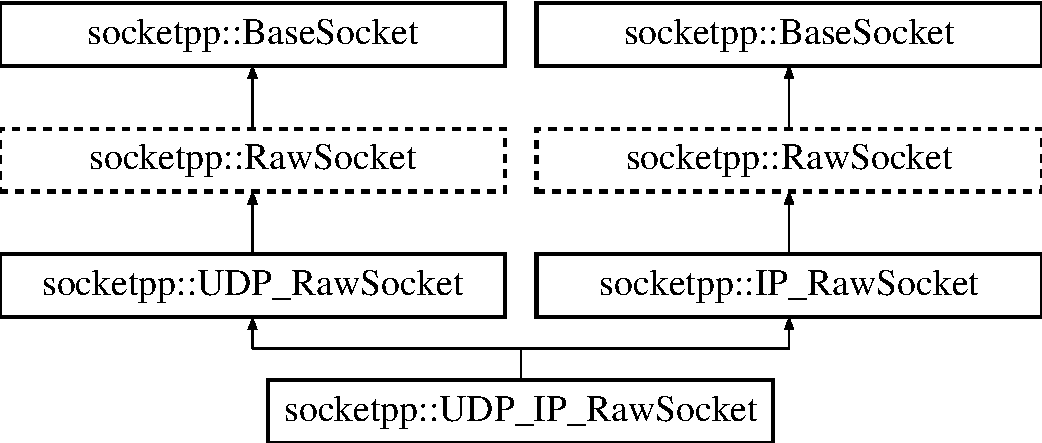
\includegraphics[height=4cm]{classsocketpp_1_1UDP__IP__RawSocket}
\end{center}
\end{figure}
\subsection*{Public Member Functions}
\begin{CompactItemize}
\item 
\hyperlink{classsocketpp_1_1UDP__IP__RawSocket_90e90d941b64d234c231ca543fe8745a}{UDP\_\-IP\_\-RawSocket} ()
\begin{CompactList}\small\item\em constructor which calls RawSocket(ipproto\_\-udp) and setsockopt(ip\_\-hdrincl) \item\end{CompactList}\item 
void \hyperlink{classsocketpp_1_1UDP__IP__RawSocket_6c2f6c375cec90f64fd093af37369d6a}{adjust\_\-UDP\_\-csum} ()
\begin{CompactList}\small\item\em sets UDP checksum, using source and dest IP addresses token by IP header \item\end{CompactList}\item 
void \hyperlink{classsocketpp_1_1UDP__IP__RawSocket_94bec31d8c856ccdafa083c74b8b7e58}{adjust\_\-UDP\_\-all} ()
\begin{CompactList}\small\item\em calls \hyperlink{classsocketpp_1_1UDP__RawSocket_1caa413cfe4f72d8c0aeccdcb10469b5}{adjust\_\-UDP\_\-len()} \&\& \hyperlink{classsocketpp_1_1UDP__IP__RawSocket_6c2f6c375cec90f64fd093af37369d6a}{adjust\_\-UDP\_\-csum()} \item\end{CompactList}\item 
void \hyperlink{classsocketpp_1_1UDP__IP__RawSocket_1a0f6360760f94f5c1569adde67d6d1b}{adjust\_\-UDP\_\-IP\_\-all} ()
\begin{CompactList}\small\item\em calls \hyperlink{classsocketpp_1_1UDP__IP__RawSocket_94bec31d8c856ccdafa083c74b8b7e58}{adjust\_\-UDP\_\-all()} and \hyperlink{classsocketpp_1_1IP__RawSocket_45e60510233daaa2f279d3a4706fdce5}{adjust\_\-IP\_\-all()} \item\end{CompactList}\end{CompactItemize}
\subsection*{Protected Member Functions}
\begin{CompactItemize}
\item 
void \hyperlink{classsocketpp_1_1UDP__IP__RawSocket_16035f1b701b898f0e4de44a9ac8bbb3}{\_\-build\_\-packet} (std::string \&packet)
\item 
void \hyperlink{classsocketpp_1_1UDP__IP__RawSocket_40fde867fa138b495f660864023a3eb1}{\_\-set\_\-fields} (const std::string \&packet)
\end{CompactItemize}


\subsection{Detailed Description}
UDP raw socket with IP header handling. 

\subsection{Constructor \& Destructor Documentation}
\hypertarget{classsocketpp_1_1UDP__IP__RawSocket_90e90d941b64d234c231ca543fe8745a}{
\index{socketpp::UDP\_\-IP\_\-RawSocket@{socketpp::UDP\_\-IP\_\-RawSocket}!UDP\_\-IP\_\-RawSocket@{UDP\_\-IP\_\-RawSocket}}
\index{UDP\_\-IP\_\-RawSocket@{UDP\_\-IP\_\-RawSocket}!socketpp::UDP_IP_RawSocket@{socketpp::UDP\_\-IP\_\-RawSocket}}
\subsubsection[{UDP\_\-IP\_\-RawSocket}]{\setlength{\rightskip}{0pt plus 5cm}socketpp::UDP\_\-IP\_\-RawSocket::UDP\_\-IP\_\-RawSocket ()}}
\label{classsocketpp_1_1UDP__IP__RawSocket_90e90d941b64d234c231ca543fe8745a}


constructor which calls RawSocket(ipproto\_\-udp) and setsockopt(ip\_\-hdrincl) 



\subsection{Member Function Documentation}
\hypertarget{classsocketpp_1_1UDP__IP__RawSocket_16035f1b701b898f0e4de44a9ac8bbb3}{
\index{socketpp::UDP\_\-IP\_\-RawSocket@{socketpp::UDP\_\-IP\_\-RawSocket}!\_\-build\_\-packet@{\_\-build\_\-packet}}
\index{\_\-build\_\-packet@{\_\-build\_\-packet}!socketpp::UDP_IP_RawSocket@{socketpp::UDP\_\-IP\_\-RawSocket}}
\subsubsection[{\_\-build\_\-packet}]{\setlength{\rightskip}{0pt plus 5cm}void socketpp::UDP\_\-IP\_\-RawSocket::\_\-build\_\-packet (std::string \& {\em packet})\hspace{0.3cm}{\tt  \mbox{[}protected, virtual\mbox{]}}}}
\label{classsocketpp_1_1UDP__IP__RawSocket_16035f1b701b898f0e4de44a9ac8bbb3}




Reimplemented from \hyperlink{classsocketpp_1_1IP__RawSocket_6863cc399c543073e9aa3615c3f50940}{socketpp::IP\_\-RawSocket}.\hypertarget{classsocketpp_1_1UDP__IP__RawSocket_40fde867fa138b495f660864023a3eb1}{
\index{socketpp::UDP\_\-IP\_\-RawSocket@{socketpp::UDP\_\-IP\_\-RawSocket}!\_\-set\_\-fields@{\_\-set\_\-fields}}
\index{\_\-set\_\-fields@{\_\-set\_\-fields}!socketpp::UDP_IP_RawSocket@{socketpp::UDP\_\-IP\_\-RawSocket}}
\subsubsection[{\_\-set\_\-fields}]{\setlength{\rightskip}{0pt plus 5cm}void socketpp::UDP\_\-IP\_\-RawSocket::\_\-set\_\-fields (const std::string \& {\em packet})\hspace{0.3cm}{\tt  \mbox{[}protected, virtual\mbox{]}}}}
\label{classsocketpp_1_1UDP__IP__RawSocket_40fde867fa138b495f660864023a3eb1}




Reimplemented from \hyperlink{classsocketpp_1_1IP__RawSocket_c39832f1ad83184cd5ba94c4c967f465}{socketpp::IP\_\-RawSocket}.\hypertarget{classsocketpp_1_1UDP__IP__RawSocket_94bec31d8c856ccdafa083c74b8b7e58}{
\index{socketpp::UDP\_\-IP\_\-RawSocket@{socketpp::UDP\_\-IP\_\-RawSocket}!adjust\_\-UDP\_\-all@{adjust\_\-UDP\_\-all}}
\index{adjust\_\-UDP\_\-all@{adjust\_\-UDP\_\-all}!socketpp::UDP_IP_RawSocket@{socketpp::UDP\_\-IP\_\-RawSocket}}
\subsubsection[{adjust\_\-UDP\_\-all}]{\setlength{\rightskip}{0pt plus 5cm}void socketpp::UDP\_\-IP\_\-RawSocket::adjust\_\-UDP\_\-all ()}}
\label{classsocketpp_1_1UDP__IP__RawSocket_94bec31d8c856ccdafa083c74b8b7e58}


calls \hyperlink{classsocketpp_1_1UDP__RawSocket_1caa413cfe4f72d8c0aeccdcb10469b5}{adjust\_\-UDP\_\-len()} \&\& \hyperlink{classsocketpp_1_1UDP__IP__RawSocket_6c2f6c375cec90f64fd093af37369d6a}{adjust\_\-UDP\_\-csum()} 

\hypertarget{classsocketpp_1_1UDP__IP__RawSocket_6c2f6c375cec90f64fd093af37369d6a}{
\index{socketpp::UDP\_\-IP\_\-RawSocket@{socketpp::UDP\_\-IP\_\-RawSocket}!adjust\_\-UDP\_\-csum@{adjust\_\-UDP\_\-csum}}
\index{adjust\_\-UDP\_\-csum@{adjust\_\-UDP\_\-csum}!socketpp::UDP_IP_RawSocket@{socketpp::UDP\_\-IP\_\-RawSocket}}
\subsubsection[{adjust\_\-UDP\_\-csum}]{\setlength{\rightskip}{0pt plus 5cm}void socketpp::UDP\_\-IP\_\-RawSocket::adjust\_\-UDP\_\-csum ()}}
\label{classsocketpp_1_1UDP__IP__RawSocket_6c2f6c375cec90f64fd093af37369d6a}


sets UDP checksum, using source and dest IP addresses token by IP header 

\hypertarget{classsocketpp_1_1UDP__IP__RawSocket_1a0f6360760f94f5c1569adde67d6d1b}{
\index{socketpp::UDP\_\-IP\_\-RawSocket@{socketpp::UDP\_\-IP\_\-RawSocket}!adjust\_\-UDP\_\-IP\_\-all@{adjust\_\-UDP\_\-IP\_\-all}}
\index{adjust\_\-UDP\_\-IP\_\-all@{adjust\_\-UDP\_\-IP\_\-all}!socketpp::UDP_IP_RawSocket@{socketpp::UDP\_\-IP\_\-RawSocket}}
\subsubsection[{adjust\_\-UDP\_\-IP\_\-all}]{\setlength{\rightskip}{0pt plus 5cm}void socketpp::UDP\_\-IP\_\-RawSocket::adjust\_\-UDP\_\-IP\_\-all ()}}
\label{classsocketpp_1_1UDP__IP__RawSocket_1a0f6360760f94f5c1569adde67d6d1b}


calls \hyperlink{classsocketpp_1_1UDP__IP__RawSocket_94bec31d8c856ccdafa083c74b8b7e58}{adjust\_\-UDP\_\-all()} and \hyperlink{classsocketpp_1_1IP__RawSocket_45e60510233daaa2f279d3a4706fdce5}{adjust\_\-IP\_\-all()} 



The documentation for this class was generated from the following files:\begin{CompactItemize}
\item 
\hyperlink{RawSocket_8h}{RawSocket.h}\item 
\hyperlink{RawSocket_8cpp}{RawSocket.cpp}\end{CompactItemize}

\hypertarget{classsocketpp_1_1UDP__RawSocket}{
\section{socketpp::UDP\_\-RawSocket Class Reference}
\label{classsocketpp_1_1UDP__RawSocket}\index{socketpp::UDP\_\-RawSocket@{socketpp::UDP\_\-RawSocket}}
}
UDP raw socket without IP header handling.  


{\tt \#include $<$RawSocket.h$>$}

Inheritance diagram for socketpp::UDP\_\-RawSocket::\begin{figure}[H]
\begin{center}
\leavevmode
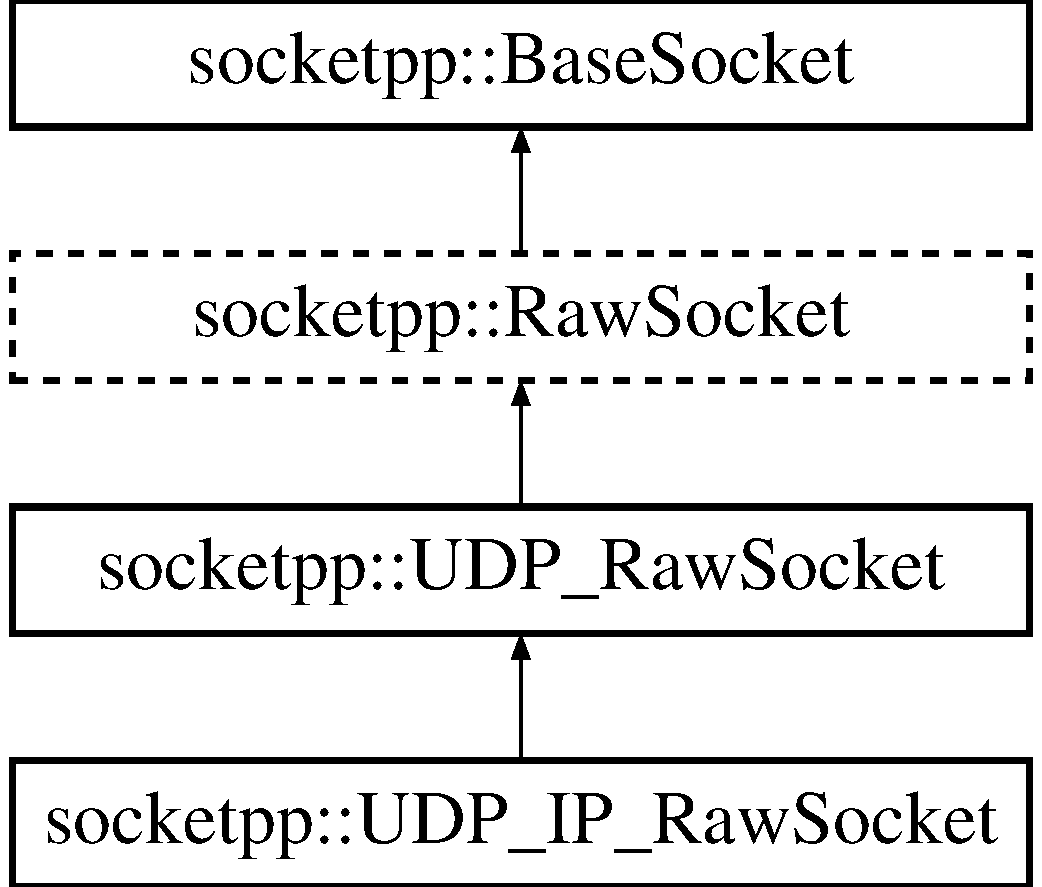
\includegraphics[height=4cm]{classsocketpp_1_1UDP__RawSocket}
\end{center}
\end{figure}
\subsection*{Public Member Functions}
\begin{CompactItemize}
\item 
\hypertarget{classsocketpp_1_1UDP__RawSocket_508aba470eee4010ca16007823c91650}{
\hyperlink{classsocketpp_1_1UDP__RawSocket_508aba470eee4010ca16007823c91650}{UDP\_\-RawSocket} ()}
\label{classsocketpp_1_1UDP__RawSocket_508aba470eee4010ca16007823c91650}

\begin{CompactList}\small\item\em constructor which calls RawSocket(ipproto\_\-udp) \item\end{CompactList}\item 
void \hyperlink{classsocketpp_1_1UDP__RawSocket_1b055bafc0e178db6a3940093dc0f8e0}{build\_\-UDP\_\-header} (\_\-u16 source, \_\-u16 dest, \_\-u16 len=0, \_\-u16 check=0)
\begin{CompactList}\small\item\em builds the internal UDP header \item\end{CompactList}\item 
void \hyperlink{classsocketpp_1_1UDP__RawSocket_b194e3ab2f5b758dee8a0c715d895c1e}{build\_\-UDP\_\-header} (const udphdr \&udp)
\begin{CompactList}\small\item\em builds the internal UDP header \item\end{CompactList}\item 
void \hyperlink{classsocketpp_1_1UDP__RawSocket_8d96a58ee9d39e2c014aa81ded23727a}{adjust\_\-UDP\_\-csum} (in\_\-addr\_\-t source, in\_\-addr\_\-t dest)
\begin{CompactList}\small\item\em sets the internal UDP pseudo-header checksum \item\end{CompactList}\item 
\hypertarget{classsocketpp_1_1UDP__RawSocket_1caa413cfe4f72d8c0aeccdcb10469b5}{
void \hyperlink{classsocketpp_1_1UDP__RawSocket_1caa413cfe4f72d8c0aeccdcb10469b5}{adjust\_\-UDP\_\-len} ()}
\label{classsocketpp_1_1UDP__RawSocket_1caa413cfe4f72d8c0aeccdcb10469b5}

\begin{CompactList}\small\item\em sets the internal header \char`\"{}len\char`\"{} field \item\end{CompactList}\item 
void \hyperlink{classsocketpp_1_1UDP__RawSocket_4fe2e6b184ca8f8248a187df30e12fd2}{adjust\_\-UDP\_\-all} (in\_\-addr\_\-t source, in\_\-addr\_\-t dest)
\begin{CompactList}\small\item\em calls \hyperlink{classsocketpp_1_1UDP__RawSocket_1caa413cfe4f72d8c0aeccdcb10469b5}{adjust\_\-UDP\_\-len()} and adjust\_\-UDP\_\-csum(source,dest) \item\end{CompactList}\item 
void \hyperlink{classsocketpp_1_1UDP__RawSocket_597a30fc537dce06c85663add29defdc}{get\_\-UDP\_\-header} (udphdr \&udp)
\begin{CompactList}\small\item\em gets the received UDP header \item\end{CompactList}\end{CompactItemize}
\subsection*{Static Public Member Functions}
\begin{CompactItemize}
\item 
static \_\-u16 \hyperlink{classsocketpp_1_1UDP__RawSocket_095971358f1de99857aaf649aae9b1ea}{udp\_\-checksum} (const struct udphdr \&udp, in\_\-addr\_\-t saddr, in\_\-addr\_\-t daddr, const void $\ast$payload=NULL, size\_\-t psize=0)
\begin{CompactList}\small\item\em calculates UDP header checksum \item\end{CompactList}\item 
static \_\-u16 \hyperlink{classsocketpp_1_1UDP__RawSocket_331a9aa1b1bc9aa16a25954061c04551}{udp\_\-checksum} (const struct udphdr \&udp, in\_\-addr\_\-t saddr, in\_\-addr\_\-t daddr, const std::string \&payload)
\begin{CompactList}\small\item\em calculates UDP header checksum \item\end{CompactList}\end{CompactItemize}
\subsection*{Protected Member Functions}
\begin{CompactItemize}
\item 
\hypertarget{classsocketpp_1_1UDP__RawSocket_9f087a8fe3d6e62397911657c6b10d29}{
virtual void \textbf{\_\-build\_\-packet} (std::string \&packet) const }
\label{classsocketpp_1_1UDP__RawSocket_9f087a8fe3d6e62397911657c6b10d29}

\item 
\hypertarget{classsocketpp_1_1UDP__RawSocket_a2dd7ab190a6730f9272eced4e648b50}{
virtual void \textbf{\_\-set\_\-fields} (const std::string \&packet)}
\label{classsocketpp_1_1UDP__RawSocket_a2dd7ab190a6730f9272eced4e648b50}

\end{CompactItemize}
\subsection*{Static Protected Member Functions}
\begin{CompactItemize}
\item 
\hypertarget{classsocketpp_1_1UDP__RawSocket_400dfa2f567ecd89df1f14f08bbb44ac}{
static void \textbf{\_\-udp\_\-convert} (const struct udphdr \&, struct udphdr \&)}
\label{classsocketpp_1_1UDP__RawSocket_400dfa2f567ecd89df1f14f08bbb44ac}

\end{CompactItemize}
\subsection*{Protected Attributes}
\begin{CompactItemize}
\item 
\hypertarget{classsocketpp_1_1UDP__RawSocket_fbdcc519279aec772f575237ca25f783}{
udphdr \textbf{UDP\_\-h}}
\label{classsocketpp_1_1UDP__RawSocket_fbdcc519279aec772f575237ca25f783}

\item 
\hypertarget{classsocketpp_1_1UDP__RawSocket_9b21e1b520434f7b07d5afcc35ceb76c}{
udphdr \textbf{rcvd\_\-UDP\_\-h}}
\label{classsocketpp_1_1UDP__RawSocket_9b21e1b520434f7b07d5afcc35ceb76c}

\end{CompactItemize}


\subsection{Detailed Description}
UDP raw socket without IP header handling. 

\subsection{Member Function Documentation}
\hypertarget{classsocketpp_1_1UDP__RawSocket_4fe2e6b184ca8f8248a187df30e12fd2}{
\index{socketpp::UDP\_\-RawSocket@{socketpp::UDP\_\-RawSocket}!adjust\_\-UDP\_\-all@{adjust\_\-UDP\_\-all}}
\index{adjust\_\-UDP\_\-all@{adjust\_\-UDP\_\-all}!socketpp::UDP_RawSocket@{socketpp::UDP\_\-RawSocket}}
\subsubsection[{adjust\_\-UDP\_\-all}]{\setlength{\rightskip}{0pt plus 5cm}void socketpp::UDP\_\-RawSocket::adjust\_\-UDP\_\-all (in\_\-addr\_\-t {\em source}, \/  in\_\-addr\_\-t {\em dest})}}
\label{classsocketpp_1_1UDP__RawSocket_4fe2e6b184ca8f8248a187df30e12fd2}


calls \hyperlink{classsocketpp_1_1UDP__RawSocket_1caa413cfe4f72d8c0aeccdcb10469b5}{adjust\_\-UDP\_\-len()} and adjust\_\-UDP\_\-csum(source,dest) 

\begin{Desc}
\item[Parameters:]
\begin{description}
\item[{\em source}]IP source address \item[{\em dest}]IP destination address \end{description}
\end{Desc}
\hypertarget{classsocketpp_1_1UDP__RawSocket_8d96a58ee9d39e2c014aa81ded23727a}{
\index{socketpp::UDP\_\-RawSocket@{socketpp::UDP\_\-RawSocket}!adjust\_\-UDP\_\-csum@{adjust\_\-UDP\_\-csum}}
\index{adjust\_\-UDP\_\-csum@{adjust\_\-UDP\_\-csum}!socketpp::UDP_RawSocket@{socketpp::UDP\_\-RawSocket}}
\subsubsection[{adjust\_\-UDP\_\-csum}]{\setlength{\rightskip}{0pt plus 5cm}void socketpp::UDP\_\-RawSocket::adjust\_\-UDP\_\-csum (in\_\-addr\_\-t {\em source}, \/  in\_\-addr\_\-t {\em dest})}}
\label{classsocketpp_1_1UDP__RawSocket_8d96a58ee9d39e2c014aa81ded23727a}


sets the internal UDP pseudo-header checksum 

\begin{Desc}
\item[Parameters:]
\begin{description}
\item[{\em source}]IP source address \item[{\em dest}]IP destination address \end{description}
\end{Desc}
\hypertarget{classsocketpp_1_1UDP__RawSocket_b194e3ab2f5b758dee8a0c715d895c1e}{
\index{socketpp::UDP\_\-RawSocket@{socketpp::UDP\_\-RawSocket}!build\_\-UDP\_\-header@{build\_\-UDP\_\-header}}
\index{build\_\-UDP\_\-header@{build\_\-UDP\_\-header}!socketpp::UDP_RawSocket@{socketpp::UDP\_\-RawSocket}}
\subsubsection[{build\_\-UDP\_\-header}]{\setlength{\rightskip}{0pt plus 5cm}void socketpp::UDP\_\-RawSocket::build\_\-UDP\_\-header (const udphdr \& {\em udp})}}
\label{classsocketpp_1_1UDP__RawSocket_b194e3ab2f5b758dee8a0c715d895c1e}


builds the internal UDP header 

\begin{Desc}
\item[Parameters:]
\begin{description}
\item[{\em udp}]UDP header \end{description}
\end{Desc}
\hypertarget{classsocketpp_1_1UDP__RawSocket_1b055bafc0e178db6a3940093dc0f8e0}{
\index{socketpp::UDP\_\-RawSocket@{socketpp::UDP\_\-RawSocket}!build\_\-UDP\_\-header@{build\_\-UDP\_\-header}}
\index{build\_\-UDP\_\-header@{build\_\-UDP\_\-header}!socketpp::UDP_RawSocket@{socketpp::UDP\_\-RawSocket}}
\subsubsection[{build\_\-UDP\_\-header}]{\setlength{\rightskip}{0pt plus 5cm}void socketpp::UDP\_\-RawSocket::build\_\-UDP\_\-header (\_\-u16 {\em source}, \/  \_\-u16 {\em dest}, \/  \_\-u16 {\em len} = {\tt 0}, \/  \_\-u16 {\em check} = {\tt 0})}}
\label{classsocketpp_1_1UDP__RawSocket_1b055bafc0e178db6a3940093dc0f8e0}


builds the internal UDP header 

\begin{Desc}
\item[Parameters:]
\begin{description}
\item[{\em source}]source port \item[{\em dest}]destination port \item[{\em len}]UDP+data total length in bytes \item[{\em check}]UDP pseudo-checksum \end{description}
\end{Desc}
\hypertarget{classsocketpp_1_1UDP__RawSocket_597a30fc537dce06c85663add29defdc}{
\index{socketpp::UDP\_\-RawSocket@{socketpp::UDP\_\-RawSocket}!get\_\-UDP\_\-header@{get\_\-UDP\_\-header}}
\index{get\_\-UDP\_\-header@{get\_\-UDP\_\-header}!socketpp::UDP_RawSocket@{socketpp::UDP\_\-RawSocket}}
\subsubsection[{get\_\-UDP\_\-header}]{\setlength{\rightskip}{0pt plus 5cm}void socketpp::UDP\_\-RawSocket::get\_\-UDP\_\-header (udphdr \& {\em udp})}}
\label{classsocketpp_1_1UDP__RawSocket_597a30fc537dce06c85663add29defdc}


gets the received UDP header 

\begin{Desc}
\item[Parameters:]
\begin{description}
\item[{\em udp}]header to modify \end{description}
\end{Desc}
\hypertarget{classsocketpp_1_1UDP__RawSocket_331a9aa1b1bc9aa16a25954061c04551}{
\index{socketpp::UDP\_\-RawSocket@{socketpp::UDP\_\-RawSocket}!udp\_\-checksum@{udp\_\-checksum}}
\index{udp\_\-checksum@{udp\_\-checksum}!socketpp::UDP_RawSocket@{socketpp::UDP\_\-RawSocket}}
\subsubsection[{udp\_\-checksum}]{\setlength{\rightskip}{0pt plus 5cm}\_\-u16 socketpp::UDP\_\-RawSocket::udp\_\-checksum (const struct udphdr \& {\em udp}, \/  in\_\-addr\_\-t {\em saddr}, \/  in\_\-addr\_\-t {\em daddr}, \/  const std::string \& {\em payload})\hspace{0.3cm}{\tt  \mbox{[}static\mbox{]}}}}
\label{classsocketpp_1_1UDP__RawSocket_331a9aa1b1bc9aa16a25954061c04551}


calculates UDP header checksum 

\begin{Desc}
\item[Parameters:]
\begin{description}
\item[{\em udp}]UDP header \item[{\em saddr}]source address \item[{\em daddr}]destination address \item[{\em payload}]data payload field \end{description}
\end{Desc}
\begin{Desc}
\item[Returns:]checksum value \end{Desc}
\hypertarget{classsocketpp_1_1UDP__RawSocket_095971358f1de99857aaf649aae9b1ea}{
\index{socketpp::UDP\_\-RawSocket@{socketpp::UDP\_\-RawSocket}!udp\_\-checksum@{udp\_\-checksum}}
\index{udp\_\-checksum@{udp\_\-checksum}!socketpp::UDP_RawSocket@{socketpp::UDP\_\-RawSocket}}
\subsubsection[{udp\_\-checksum}]{\setlength{\rightskip}{0pt plus 5cm}\_\-u16 socketpp::UDP\_\-RawSocket::udp\_\-checksum (const struct udphdr \& {\em udp}, \/  in\_\-addr\_\-t {\em saddr}, \/  in\_\-addr\_\-t {\em daddr}, \/  const void $\ast$ {\em payload} = {\tt NULL}, \/  size\_\-t {\em psize} = {\tt 0})\hspace{0.3cm}{\tt  \mbox{[}static\mbox{]}}}}
\label{classsocketpp_1_1UDP__RawSocket_095971358f1de99857aaf649aae9b1ea}


calculates UDP header checksum 

\begin{Desc}
\item[Parameters:]
\begin{description}
\item[{\em udp}]UDP header \item[{\em saddr}]source address \item[{\em daddr}]destination address \item[{\em payload}]pointer to data payload field \item[{\em psize}]data payload size \end{description}
\end{Desc}
\begin{Desc}
\item[Returns:]checksum value \end{Desc}


The documentation for this class was generated from the following files:\begin{CompactItemize}
\item 
RawSocket.h\item 
RawSocket.cpp\end{CompactItemize}

\printindex
\end{document}
